\documentclass{cmspaper}
\usepackage{graphicx}
\usepackage{appendix}
\usepackage{rotate}
\usepackage{relsize}
\usepackage{amsmath}
\usepackage{amssymb}
\usepackage{cite}

\newcommand{\met} {\ensuremath{E\!\!\!\!/_T}}
\newcommand{\ttbar} {\ensuremath{t\bar{t}~}}
\newcommand{\ptll} {\ensuremath{P_T(\ell\ell)}}
\newcommand{\ptllres} {\ensuremath{P^{\rm res}_T(\ell\ell)}}

\begin{document}

%==============================================================================
% title page for many authors
%
\begin{titlepage}
\title{Interpreting CMS data in the phenomenological MSSM}

  \begin{Authlist}
    Maurizio Pierini
    \Instfoot{cern}{CERN}    
    Maria Spiropulu
    \Instfoot{caltech}{CERN \& California Institute Of Technology, Pasadena}    
    Filip Moortgat, Luc Pape
    \Instfoot{eth}{ETH, Zurich, Switzerland}
    Joseph Lykken
    \Instfoot{fnal}{Fermi National Accelerator Laboratory, Batavia, Illinois}
    Harrison Prosper, Sezen Sekmen
    \Instfoot{fsu}{Florida State University, Tallahassee}
    Sabine Kraml
    \Instfoot{lpsc}{LPSC Grenoble, France}
    Sanjay Padhi
    \Instfoot{ucsd}{University of California, San Diego}
    
  \end{Authlist}

\begin{abstract}
We interpret the data taken with the CMS detector during the 7 TeV LHC run within the phenomenological MSSM (pMSSM). 
The pMSSM is a 19-dimensional parametrization of the MSSM that captures most of its phenomenological features. The 19-dimensional model
encompasses, and goes beyond, a broad range of more constrained SUSY models (such as the CMSSM). 
Using profile likelihoods, we examine the influence of each of the 
19 parameters and determine to which parameters 
(and predicted observables) the current CMS data are most sensitive. 
We provide constraints on quantities sensitive to hadronic as well as multi-lepton final states, 
based on the 2010 CMS data-set corresponding to 35~pb$^{-1}$ of integrated luminosity.
In contrast to constraints derived for particular SUSY breaking schemes 
such as the CMSSM, our results provide more generic conclusions on how the current 
data constrain the MSSM. 
Moreover, while the focus of this note is the 
MSSM, the approach we describe is applicable to \emph{any} multi-parameter model.
\end{abstract}
\end{titlepage}

\section{Introduction}
\label{sec:intro}

After the successful operation of the Large Hadron Collider (LHC) and the CMS detector
in 2010 and 2011, and with good prospects for the future, the LHC is now ready to shed light on a number 
of open questions in Particle Physics 
such as the mechanism of electroweak (EW) symmetry breaking, or the 
new physics, Beyond the Standard Model (BSM), that stabilizes the EW scale. 

A wealth of theories that extend the Standard Model have been put forth during the past decades. Supersymmetry (SUSY) is
arguably the best motivated BSM theory --- and certainly the most 
thoroughly studied. 
Indeed, searches for SUSY are among the primary objectives of the 
CMS experiment. SUSY is exceedingly popular not 
only for its theoretical beauty but also because SUSY phenomenology 
is extremely rich, 
%in fact is can mimic almost any other new physics scenario. 
leading to a large variety of possible new signals at the LHC. 
In spite of this, the majority of SUSY studies focus on a very special 
setup: the so-called Constrained Minimal Supersymmetric Standard Model (CMSSM). 
This was justified in the preparation for discoveries as the CMSSM, 
having just a handful of new parameters, is very predicive. However, 
the simplifying assumption of universality at the GUT scale lacks a sound 
theoretical motivation. Consequently, the CMSSM should be regarded as a showcase 
model. When it comes to interpreting experimental results, it is reasonable and interesting to do this within the CMSSM because it 
provides (to some degree) an easy way to show performances, 
compare limits or reaches, etc. However, the interpretation of experimental results in the 
$(m_0,m_{1/2})$ plane risks imposing unwarranted constraints on SUSY, as many 
mass patterns and signatures that are possible a priori are not covered in the CMSSM. 
The same problem arises in any analysis that assumes a particular 
SUSY breaking scheme. 

In this document, we therefore introduce a different approach, which uses only 
minimal assumptions on the underlying SUSY parameters. In particular, given the absence of experimental guidance, we choose
not to rely on a particular SUSY breaking scheme.
Instead, we use a 19-dimensional 
parametrization of the MSSM, called the \emph{phenomenological MSSM} (pMSSM),
with parameters defined not at the GUT scale but instead at the SUSY scale 
(by convention the geometric mean of the two stop masses).
We demonstrate the feasibility of our approach by applying it to 
the 2011 CMS data-set corresponding to 1~fb$^{-1}$ of integrated luminosity.  
Using profile likelihoods, we combine 
the dijet $\alpha_T$ analysis, the opposite-sign dilepton 
analysis and the same-sign dilepton analysis and derive constraints 
on the SUSY particles with as few simplifying assumptions as possible.
Results from other SUSY analyses in CMS will be added as soon as they become available.

We first give the motivation to go beyond the CMSSM and work in 
a generic MSSM setup. After this, the pMSSM and its parametrization is defined. 
We then outline our analysis, giving details on the pMSSM points we have used, 
the detector simulation and the CMS analyses, and describe the statistical method based on 
profile likelihoods used for coping with the 19-dimensional model. Finally, we discuss our results and summarize our conclusions.


\section{Motivation for a generic MSSM setup}
\label{sec:motivation}

Perhaps the least understood aspect of SUSY is its breaking, 
which in turn determines the boundary conditions for the Lagrange 
parameters at some high scale. Theorists have come up with a 
long list of possible candidate scenarios, including 
supergravity (SUGRA), 
gauge mediation (GMSB), 
anomaly mediation (AMSB), 
gaugino mediation, radion mediation, etc.. 
They come in minimal (mSUGRA, mGMSB, ....) and  
less minimal ({\it e.g.}, non-universal Higgs masses, NUHM,  
or non-universal gaugino masses) variants, as well as in general setups 
(general gauge mediation, ...). 
Moreover, there are models of compressed, effective or split SUSY, 
GUT-inspired models, string-inspired models, and so on. 
Each of these possibilities features characteristic relations between 
fundamental parameters and hence characteristic mass spectra, decay 
patterns and properties of the dark matter candidate. 

The CMSSM covers just a subset of this spectrum. To give some 
examples:

\begin{itemize}

\item The CMSSM assumes universal gaugino masses $M_1=M_2=M_3\equiv m_{1/2}$ 
at the GUT scale, leading to 
\begin{equation}
  M_1 : M_2 : M_3 \approx 1 : 2 : 7 ~{\rm with}~ M_1 \approx 0.4\,m_{1/2}
  \label{eq:gauginos}
\end{equation}
at the EW scale, which is equivalent to 
$m_{\tilde\chi^0_2}\approx 2m_{\tilde\chi^0_1}\approx 0.8\,m_{1/2}$ 
and $m_{\tilde g}\approx 7m_{\tilde\chi^0_1}\approx 2.8\,m_{1/2}$. 
Other models can have very different relations between 
$M_1$, $M_2$, $M_3$, giving rise to the so-called 
``gaugino code''~\cite{Choi:2007ka}, 
which can be very useful for model discrimination. Besides, models with 
non-universal gaugino masses are quite natural~\cite{Martin:2009ad} even 
within the SUGRA context, and they can have very low finetuning~\cite{Horton:2009ed}.

\item Over most of the CMSSM parameter space $|\mu|^2\gtrsim m_{1/2}^2$. 
The lightest neutralino is then mostly bino, the second-lightest mostly wino, 
and the heavier ones mostly higgsinos. Light higgsinos and large gaugino--higgsino 
mixing (mixed bino--higgsino dark matter) occur only in the focus point region, 
{\it i.e.}\ when squarks and sleptons are very heavy. This has a strong impact on 
squark and gluino cascade decays, as well as on the part of parameter 
space that is compatible with dark matter constraints. 

\item Turning to the sfermion sector, the slepton-mass parameters are to good approximation
\begin{equation}
  m_{\tilde E}^2 \approx m_0^2 + 0.15\,m_{1/2}^2\,, \qquad 
  m_{\tilde L}^2 \approx m_0^2 + 0.5\,m_{1/2}^2\,. 
  \label{eq:sleptons}
\end{equation}
Note that this implies that right-chiral states are alway lighter 
than the left-chiral ones. Combining Eqs.~(\ref{eq:gauginos}) and 
(\ref{eq:sleptons}) we see that for small $m_0$ (but large enough 
to have a neutralino LSP) this leads to the typical mass pattern 
$m_{\tilde\chi^0_1}<m_{\tilde e_R}<m_{\tilde\chi^0_2}<m_{\tilde e_L}$.  
For the first two generations of squarks we have 
\begin{equation}
  m_{\tilde U, \tilde D}^2 \approx m_0^2 + K m_{1/2}^2\,, \qquad 
  m_{\tilde Q}^2 \approx m_0^2 + (K+0.5)m_{1/2}^2\,, 
\end{equation}
with $K\sim4.5$ to $6.5$, and the dependence on $m_{1/2}$ dominated by the 
gluino contribution, {\it i.e.}\ by $M_3$. It is clear that any limit on 
or determination of $m_0$ is completely dominated by the slepton 
sector~\cite{Allanach:2006fy}. 
Non-universal scalar masses are heavily constrained by flavour-changing 
neutral currents (FCNC), at least for the first and second generations. 
For the third generation, the FCNC constraints are much less severe. 
One possibility to motivate universal mass parameters for sfermions is 
to embed them in a higher gauge group, like SO(10). But even then, 
non-universalities can occur through D-term contributions \cite{Kolda:1995iw} 
and/or GUT-scale threshold corrections \cite{Polonsky:1994sr,Polonsky:1994rz}. 
Besides, there is no sound theoretical motivation for unifying the 
mass-squared terms of the Higgs fields, $m_{H_1}^2$ and $m_{H_2}^2$,
with those of the other scalars. 
If this is given up $m_{H_{1,2}}^2$, or equivalently $\mu$ and $m_A$,
become free parameters of the model~\cite{Ellis:2002wv} 
(cf.\ the discussion of the value of $\mu$ above).

\item The assumption of scalar mass universality has another important 
implication, namely that the renormalization-group invariant quantity  
\begin{equation}
  S = \left(m_{H_2}^2-m_{H_1}^2\right) + {\rm Tr}\left(
      m_{\tilde Q}^2-2m_{\tilde U}^2+m_{\tilde D}^2
      +m_{\tilde E}^2-m_{\tilde L}^2\right)
\end{equation}
vanishes. This so-called $S$-parameter, if non-zero, influences 
the running of the scalar mass parametres $m_\phi^2$ proportional to 
their hypercharge $Y_\phi$
\begin{equation}
   16\pi^2\frac{d}{dt}m_\phi^2= .... + \frac{6}{5}Y_\phi g_1^2S\,.
\end{equation}
This can change the mass ordering of left- and right-chiral states 
or have an important influence on the Higgs sector. 
In the CMSSM however $S\equiv 0$.

\end{itemize}

From these considerations, which are just exemplary and by no means complete, 
it is clear that it is interesting and necessary to go beyond the na\"ive 
CMSSM. We need to search for SUSY without prejudice \cite{Berger:2008cq,Conley:2010du},  
even more so as we have all the necessary knowledge and machinery at 
our disposal. In this context note that major efforts have recently been 
devoted to developing precise statistical tools for analyzing new physics 
at the LHC \cite{Lyons:2003bw}. 
This includes sophisticated methods and tools for the investigation of 
multi-dimensional parameter spaces, as typical for SUSY models. 
Below we therefore lay out a program for the investigation of the 
phenomenological MSSM, which gets by with only a minimal set of assumptions. 
Most importantly it allows us to cover the full range of possible mass patterns 
and of neutralino dark matter properties.

\section{Phenomenological MSSM (pMSSM)}
\label{sec:model}

As mentioned, the pMSSM is a 19-dimensional realization of the MSSM 
with parameters defined at the so-called SUSY scale\footnote{Sometimes 
also referred to as the scale of electroweak symmetry breaking, $M_{\rm EWSB}$.} 
$M_{\rm SUSY}=\sqrt{m_{\tilde t_1}m_{\tilde t_2}}$. How do we come to 
this number of parameters and what are its implications?

In its most generic form, just assuming R-parity conservation, 
the MSSM has over 120 free parameters: 
SUSY-breaking mass terms and trilinear couplings, Yukawa matrices, 
CP phases, two VEVs, and a superpotential $\mu$ term. 
Model builders construct theoretically-motivated economic models 
that provide relations between these parameters at some high scale, 
{\it e.g.}, the GUT scale. 
These then evolved to $M_{\rm SUSY}$ by renormalization group equations 
to derive model-specific testable predictions. On the other 
hand, it is expected that once SUSY particles are discovered, measurements 
of their masses and interactions will allow to reconstruct (at least 
part of) the Lagrange parameters and thus infer the underlying SUSY 
breaking mechanism.
 
Luckily not all of the $\sim$120 MSSM parameters are of equal relevance to this end.
In fact, a couple of reasonable assumptions motivated by experiment serve to 
simplify the problem a lot. In particular, it is reasonable to restrict ourselves 
to the CP-conserving MSSM ({\it i.e.}\ no new CP phases) with minimal flavor violation (MFV).  
Constraints from the flavor sector moreover suggest that the first two generations 
of sfermions be taken to be degenerate. Regarding Yukawa and trilinear couplings, 
only those of the third generation matter at leading order. 
Finally, we assume that the gravitino is heavy\footnote{To be completely honest, 
this implies after all some assumption on the SUSY breaking mechanism; for instance it 
excludes low-scale gauge mediation.} and the lightest supersymmetric 
particle (LSP) is the lightest neutralino, $\tilde\chi^0_1$.
 
This leaves us with the 19 real, weak-scale SUSY Lagrange parameters 
that define the pMSSM:
\begin{itemize}
   \item 3 gaugino masses $M_1$, $M_2$, and $M_3$ 
         (pertaining to U(1), SU(2), and SU(3) gauginos, respectively);         
   \item the higgsino mass parameter $\mu$;
   \item the ratio of the Higgs VEVs $\tan\beta=v_2/v_1$;
   \item the pseudo-scalar Higgs mass $m_A$;\footnote{The parameters $\mu$ and $m_A$  
         can be swapped for the Higgs mass parameters $m_{H_1}^2$ and $m_{H_2}^2$.}
   \item 10 sfermion mass parameters $m_{\tilde{F}}$, where 
         $\tilde{F} = \tilde{Q}_1, \tilde{U}_1, \tilde{D}_1, 
                      \tilde{L}_1, \tilde{E}_1, 
                      \tilde{Q}_3, \tilde{U}_3, \tilde{D}_3, 
                      \tilde{L}_3$, and $\tilde{E}_3$ \\ 
(recall that $m_{\tilde{Q}_1}\equiv m_{\tilde{Q}_2}$, 
           $m_{\tilde{L}_1}\equiv m_{\tilde{L}_2}$, etc.); and          
   \item 3 trilinear couplings $A_t$, $A_b$ and $A_\tau$                  
\end{itemize}
 
In \cite{Berger:2008cq}, Berger {\it et al.}\ performed a scan of the pMSSM parameters  
to find out what regions of parameter space are consistent with theoretical and experimental constrains. In particular they did a uniform random sampling of 
points from within the following ranges:\footnote{Here note that $M_1$, $M_2$, 
$\mu$, $A_t$, $A_b$ and $A_\tau$ can have 
arbitrary signs; $M_3$ was chosen to be positive because only six 
of all possible sign combinations of $M_i$, $A_i$, $\mu$ are physical.} 
\begin{eqnarray}
  \mbox{100 GeV} \leq 	& m_{\tilde{F}}  & \leq \mbox{1000 GeV},   \nonumber \\
  \mbox{50 GeV}  \leq	& |M_{1,2},\mu|  & \leq \mbox{1000 GeV}, 	 \nonumber \\
  \mbox{100 GeV} \leq	& M_3 	     & \leq \mbox{1000 GeV},   \\
	                  & |A_{t,b,\tau}| & \leq \mbox{1000 GeV}, 	 \nonumber \\
    1  \leq			& \tan\beta		& \leq 50,	  \nonumber \\
    \mbox{43.5 GeV}	\leq	& m_A			& \leq \mbox{1000 GeV},  \nonumber 
\end{eqnarray}

Imposing SUSY and Higgs mass limits and requiring consistency with low-energy 
constraints and with the dark matter relic density, 
they found \cite{Berger:2008cq} that 
{\it ``the pMSSM leads to a much broader set of predictions for the properties 
of the SUSY partners as well as for a number of experimental observables than 
those found in any of the conventional SUSY breaking scenarios such as mSUGRA [CMSSM]. This set of models can easily lead to atypical expectations for SUSY signals 
at the LHC.''}

As a first step towards a full pMSSM analysis, we use a 6K subset of the 
pMSSM points generated by Berger {\it et al.}\ and investigate to which 
extent CMS SUSY analyses with 35~pb$^{-1}$ of data already constrain 
this sample. 

%\section{Current experimental and theoretical constraints}
\label{sec:limits}

The most relevant constraints today are the [SUSY and Higgs] mass 
limits from LEP2 and the Tevatron, electroweak precision observables, 
the branching ratios of the decays 
$B\to X_s\gamma$ and $B_s\to \mu^+\mu^-$, the anomalous magnetic moment of the 
muon $(g-2)_\mu$, and the relic density of dark matter $\Omega h^2$.  
They are compiled in Table~\ref{tab:observables} (to be extended).

Other important constraints, which we are not yet taking into account, 
come from $m_W$, $A^{\rm FB}_b$ and $\Delta M_{b}$.


\begin{table}[h]\begin{center}
\begin{tabular}{| l | c | c || c | l |}
  \hline
  Observable & exp.\ constraint & ref. & add. theory error & ref. \\ 
  \hline
  $M_Z$ [GeV] & $91.1875\pm 0.0021$ 
              & \cite{Nakamura:2010zzi} & -- & \\
  $M_t$ [GeV] & $173.3\pm 1.1$ 
              & \cite{top:1900yx} & -- & \\
  $\mbmb$ [GeV] &  $4.19^{+0.18}_{-0.06}$ 
                & \cite{Nakamura:2010zzi} & -- & \\
  $\asmz$ & $0.1184\pm 0.0007$ & \cite{Nakamura:2010zzi} & -- & \\
          & or $0.1176\pm 0.002$ & \cite{Nakamura:2010zzi} & -- & \\
  \hline
  $m_h$ [GeV] & $\ge 114.4$ & \cite{Schael:2006cr} 
              & $\pm 1.5$ & \cite{Degrassi:2002fi} \\
  $\Delta a_\mu \times 10^{-10}$ 
       & $e^+e^-:$ $29.6\pm 8.1$ 
       & \cite{Davier:2010nc} & $\pm 2$ & \\
       & $\tau's:$ $15.7\pm 8.2$ 
       & \cite{xxx} &  & \\
  ${\rm BR}(b\to s\gamma)\times 10^{-4}$  
       & $3.55 \pm 0.24_{\rm stat}\pm 0.09_{\rm sys}$  
       & \cite{HFAG:2010qj}  & ? &  \\
  ${\rm BR}(B_s\to \mu^+\mu^-)$  
       & $\le 3.6 \times 10^{-8}$ & \cite{HFAG:2010qj} & ? &  \\
  $\Omega_{\rm DM} h^2$ 
       & $0.1123\pm 0.0035$ 
       & \cite{Jarosik:2010iu} 
       & ? &   \\
  SUSY masses & LEP2 limits 
              & \cite{lepsusy} 
	      & ? & \\
  \hline
\end{tabular}
\end{center}
\caption{\label{tab:observables} Important observables, to be used in the likelihood calculation. }
\end{table}


\section{Analysis}
\label{sec:analysis}

As a first step towards a full pMSSM analysis, we use a 6K subset of the 
pMSSM points generated by Berger {\it et al.}\ and investigate to what
extent current CMS SUSY analyses with 35~pb$^{-1}$ of data already constrain the 
19-dimensional parameter space of the pMSSM.
To achieve this goal, we carry out the following analysis steps:
\begin{itemize}
\item For each of the 6K pMSSM points we generate 10K events.
\item We perform three blessed CMS analyses, namely the
 ``di-jet $\alpha_T$" (Had), ``opposite-sign di-lepton" (OS) and ``same-sign di-lepton" (SS) 
 analyses on each of the 6K pMSSM samples.
\item For each pMSSM point and for each of the three analyses, we combine the 
predicted signal yield $s$ with the approved CMS results---the
observed event count $N$ and 
a data-driven background estimate $b \pm \delta b$---to compute the likelihood as a function
of the pMSSM parameters. 
\item We weight every pMSSM point with the product of the three likelihoods, one  for each
of the three analyses. Since the pMSSM points were sampled from a (bounded) 
uniform  19-dimensional density, the set of weights constitute a non-parametric 
representation of the likelihood function. 
\item In order to illustrate the contribution of the current CMS data, we calculate profile likelihoods 
for the relevant model parameters, with and without the CMS likelihood, that is, the weights.  \end{itemize}

\subsection{Event samples}

We use a 6K subset of the pMSSM points generated by Berger \emph{et al.} 
as explained in Section~\ref{sec:model}.  Information on each point is contained in a SUSY Les Houches (SLHA)~\cite{Skands:2003cj} file.  For each point, 10K events were generated using {\tt PYTHIA6}~\cite{Sjostrand:2006za}.  We simulate the response of the CMS detector using
the publicly available general purpose detector simulation package {\tt Delphes}~\cite{Ovyn:2009tx}.  Through extensive numerical and shape comparisons we
conclude that we are able to provide a \emph{very} fast simulation of the CMS detector 
that is good to within 10\%. An accurate,  fast, simulation is critical for studies
of this scope. For the leptonic studies the agreement is within 25\%. Further details on {\tt CMSSW} fullsim - {\tt Delphes} comparison can be found in Appendix~\ref{sec:cmsdelphescomp}.
During the next iteration of this study, we plan to 
use the efficiency model outlined in ~\cite{sspaper}.

\subsection{The three CMS analyses}

We use the following three blessed CMS SUSY analyses designed for the early 35 pb$^{-1}$ CMS 7 TeV data  collected in 2010:
\begin{itemize}
\item the di-jet $\alpha_T$ analysis~\cite{alphatpaper}, investigating the multijets plus missing energy final state with emphasis on the $\alpha_T$ variable proposed by Randall and Tucker-Smith,
\item the opposite-sign di-lepton analysis~\cite{ospaper}, investigating the opposite-sign di-lepton plus missing energy final state,
\item and the same-sign di-lepton analysis~\cite{sspaper}, investigating the same-sign di-lepton plus missing energy final state.
\end{itemize}
For this study, we use the observed event counts, background estimates and expected signal yields, as described in Sections~\ref{sec:dbgcount} and~\ref{sec:sigyield}.

\subsubsection{Observed event counts and background estimates}
\label{sec:dbgcount}

The $\alpha_T$ and the two di-lepton analyses were developed in detail by the CMS SUSY RA1 and RA6 groups, respectively, and applied to the 7 TeV 35 pb$^{-1}$ CMS data and 7 TeV SM and SUSY Monte Carlo event samples, 
generated and simulated centrally in 2010
using the full {\it CMSSW} simulation.
We take the observed event counts and background estimates directly from the official results of these analyses.  The numbers are summarized in Table~\ref{tab:dbgcount}.

\begin{table}[htdp]
\caption{Results of the three CMS analyses for 35 pb$^{-1}$.}
\begin{center}
\begin{tabular}{|c|c|c|c|}
\hline
Analysis & Observed    & Data-driven SM & MC SM BG \\
              & event count & BG estimate      & prediction    \\
(k)          & ($N_k$)     & ($b_k \pm \delta b_k$) & ($b_k^{MC} \pm b_k^{MC}$) \\
\hline              
Dijet $\alpha_T$ & 13 & $9.4^{+ 4.8}_{-4.0} \pm $ 1.0 $[ 10.5^{+3.6}_{-2.5} ]$ & 9.3 $\pm$ 0.9 \\
OS di-lepton & 1 & 1.4 $\pm$ 0.8 & 1.3 \\
SS di-lepton & 0 & 1.2 $\pm$ 0.8 & 0.35 \\
\hline
\end{tabular}
\end{center}
\label{tab:dbgcount}
\end{table}%


\subsubsection{Signal yields}
\label{sec:sigyield}

For each of the 6K pMSSM points, we performed the three analyses on the associated 10K simulated and reconstructed events. This results in three expected signal yields for every pMSSM point. 


\subsection{Calculation of the likelihood function}

Every analysis $k$ yields an observed count $N_k$ and a background estimate
$b_k \pm \delta b_k$ where $k=1,2,3$.  We make the standard assumption that the
counts are Poisson distributed in which case the total likelihood from the combination of the three analyses can be written as
\begin{equation}
L(\theta) \equiv p(N|s,b) = \prod_{k=1}^3 \mbox{Poisson}(N_k | s_k + b_k),
\end{equation}
where $s_k$ is the predicted signal and $L(\theta)$ the likelihood
written as a function of the  $d = $19-dimensional pMSSM parameter $\theta$. 
In this study, the
 map of $\theta$ to the expected signals $s_k$ is represented non-parametrically
 using the 6K pMSSM points. In principle, we could build a smooth functional approximation to
 this map; however, we have not attempted this in the current study. 
 We incorporate the joint likelihood function of the three CMS analyses by
 weighting the $i$th pMSSM point by the likelihood 
 value $L(\theta_i)$ for that point. Since the sampling of points is uniform, the swarm of weighted
 points constitute a non-parametric representation of $L(\theta)$.
 
 For any likelihood function, exact confidence regions~\cite{James}  can \emph{always} 
 be created in
 the unrestricted parameter space. However, such
 confidence regions are seldom useful when the dimensionality of the 
 parameter space is large. It is 
 more useful to examine parameters one or two at a time. In the current study,
 we examine each parameter separately using the profile likelihood, a broadly applicable frequentist
 construct.

\subsection{Calculation of profile likelihoods}
As noted above, an important goal of this study is to determine to which pMSSM parameters the current  CMS data-set are most sensitive and to what degree. This is useful because we shall
be able to make statements whose validity is much broader than those made using
models in which simplifying, but strong, assumptions have been made.  A well-established way of conveying relevant information about the parameters of interest
 is to display their 1-dimensional profile likelihoods. We do this for each pMSSM parameter
as well as for some observables.

Suppose we wish to investigate the gluino mass parameter $M_3$. Its 
(1-dimensional) profile likelihood, $L_p$,~\cite{James} is defined by
\begin{equation}
 L_p(M_3) \equiv L(M_3, \hat{\theta}_2(M_3),\cdots, \hat{\theta}_{19}(M_3)),
\end{equation}
where $\hat{\theta}_2\cdots\hat{\theta}_{19}$ denote the maximum likelihood 
estimates (MLE), for a given value of $M_3$, of the remaining 18 parameters. 
Since we do not have a functional approximation of the map from $\theta$ to the
expected signals, our likelihood
function $L(\theta)$ is available non-parametrically as a swarm of weighted points, so standard
maximizing programs such as {\tt MINUIT} cannot be used. We have therefore devised
our own non-parametric profiling algorithm, which proceeds as follows:
\begin{enumerate}
\item For each 1-dimensional bin of the parameter or observable of interest,
for example $M_3$, we create a $d$-dimensional histogram of the 6K points using the Root class {\tt TKDTreeBinning}. Through recursive binary partitioning, this class creates $d$-dimensional bins with equal bin content.
\item For a given bin, e.g. in the gluino mass parameter $M_3$, we find which of the 6K points is consistent with the given value of $M_3$.
\item Using these points, we find the bin with the maximum density (the one with the smallest
volume) and use that as an estimate of the profile likelihood value for the given value of $M_3$. 
\item In addition, in order to provide a better estimate, the above procedure is repeated 100 times, each with a different bootstrap sample of the original 6K points and the average is taken over the profiles in each bin. This in turn is done for each of the $\sim 70$ variables under investigation.
\end{enumerate}



\section{Results}
\label{sec:results}

We present the results obtained by following the analysis path in Section~\ref{sec:analysis}, in terms of  plots of likelihood ratios $L_p / L_{max}$ as a function of each parameter of interest.  Further details on this ratio as a  measure can be found in the Appendix.  

Plots of the likelihood ratio $L_p/L_{max}$ are shown for the 19 input pMSSM parameters in Figures~\ref{fig:LRwcms_msq} to~\ref{fig:LRwcms_tbmu}.  Similarly Figures~\ref{fig:LRwcms_sq} to~\ref{fig:LRwcms_Higgs} show the likelihood ratio for the physical sparticle masses.  The relationships between the scalar SUSY breaking mass parameters and the physical scalar masses as well as those between the gaugino mass parameters and the physical gaugino masses should be noted.  The colored and shaded histograms in each plot depict the likelihood ratio before and after the inclusion of CMS results, respectively.  We observe that the CMS results indeed introduce a variation in the likelihood ratios, where the variation is more enhanced for some parameters/masses and milder for others.  

We see that all squark/slepton mass parameters and all squark/slepton masses shift upwards systematically after the addition of CMS results.  The gaugino mass parameter $M_3$ and the gluino mass also move up simultaneously due to the constraints coming from the di-jet $\alpha_T$ analysis.  An important aspect to note is that no significant change is observed in the distribution for the mass of $\tilde{\chi}^0_1$, which is the lightest supersymmetric particle (LSP), since neither a stringent $E^T_{miss}$ cut nor any other technique dedicated to constraining the $\tilde{\chi}^0_1$ mass were imposed in the analyses considered.  We are ability to observe this effect due
to the freedom offered by the pMSSM parameterization, in which neutralino/chargino masses are allowed to vary independently of the gluino mass.  Had the interpretation been done using 
the CMSSM, we would be influenced by the strict gaugino mass relationship described in Section~\ref{sec:motivation}, and the $\tilde{\chi}^0_1$ mass would be forced to move upwards along with the gluino mass.

Figure~\ref{fig:LRwcms_omg} shows $L_p/L_{max}$ for the dark matter relic density calculated using {\tt micrOMEGAs 2.4}~\cite{Belanger:2006is} assuming $\tilde{\chi}^0_1$ is the LSP and the dark matter candidate.  It must be noted that Berger {\it et al.} imposed the WMAP upper limit $\Omega_{\tilde{\chi}^0_1}h^2 \le 0.1210$ as a constraint on the points.  Information from CMS does modify the distribution, however the effect is not sufficient to impose a concrete constraint on $\Omega_{\tilde{\chi}^0_1}h^2$.  This is of course related to the result on the $\chi^0_1$ mass.

Finally, Figures~\ref{fig:LRwcms_EWobs_s1} and~\ref{fig:LRwcms_EWobs_s2} show distributions for low energy observables as predicted by the pMSSM, calculated using {\tt micrOMEGAs 2.4} and {\tt Superiso 2.7}~\cite{Mahmoudi:2008tp}.  We again note that the constraints based on experimental measurements for a subset of these observables were imposed
by Berger {\it et al.} in their selection of the pMSSM points.  Similarly to the case for the relic density, the 2010 CMS measurements do not yet allow us to constrain these observables further.  However, the prospect of making statements on the predictions for low energy observables in the presence of more data and diverse analysis channels stands out as a strong motivation in favor of interpreting the data within the framework of supersymmetry.

The results we have presented in this Note, with only 35 pb$^{-1}$ of CMS data, show that even with a modest amount of data, we are able to start making inferences of a general nature
about supersymmetry. 
%on a sufficiently generic and well-motivated construction of supersymmetry.  
Therefore, we anticipate that at least with an order of magnitude more data, the approach we have developed will allow us to make definitive statements about a broad class of supersymmetric models.  
This is only the starting point in a vast landscape of investigation. In the near term, 
we will develop this approach further by considering the following:

\begin{itemize}
\item An improved treatment of the constraints from the EW observables.  We shall replace the box-like likelihood of Berger {\it et al.} by a more appropriate likelihood function.
\item A significant increase in the sample of pMSSM points. 
\item Inclusion of a wider range of final states.
\item The development of a more quantitative treatment of the bounds on the pMSSM parameter space.
\end{itemize}


\begin{figure}[htbp]
\begin{center}
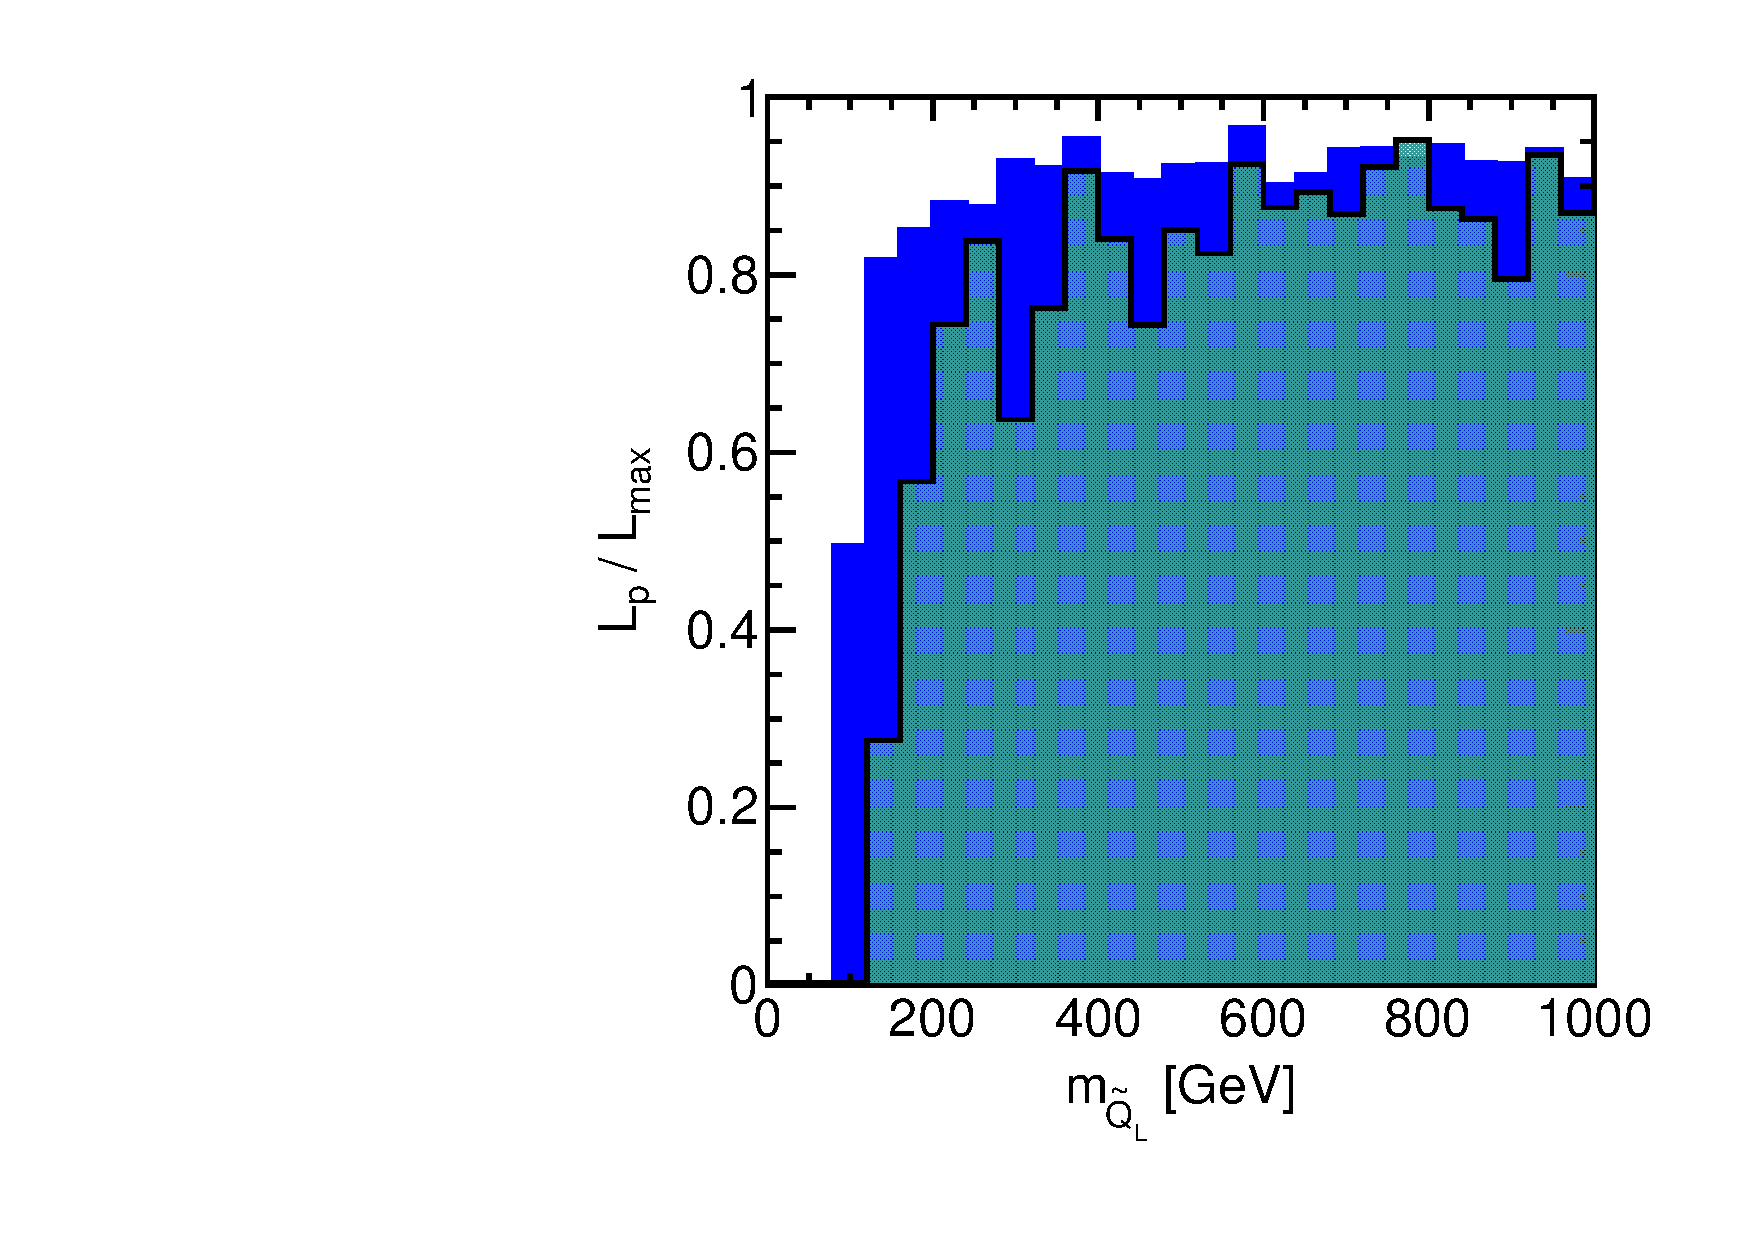
\includegraphics[height=5.5cm]{figs/fig_m_Q_L.pdf} 
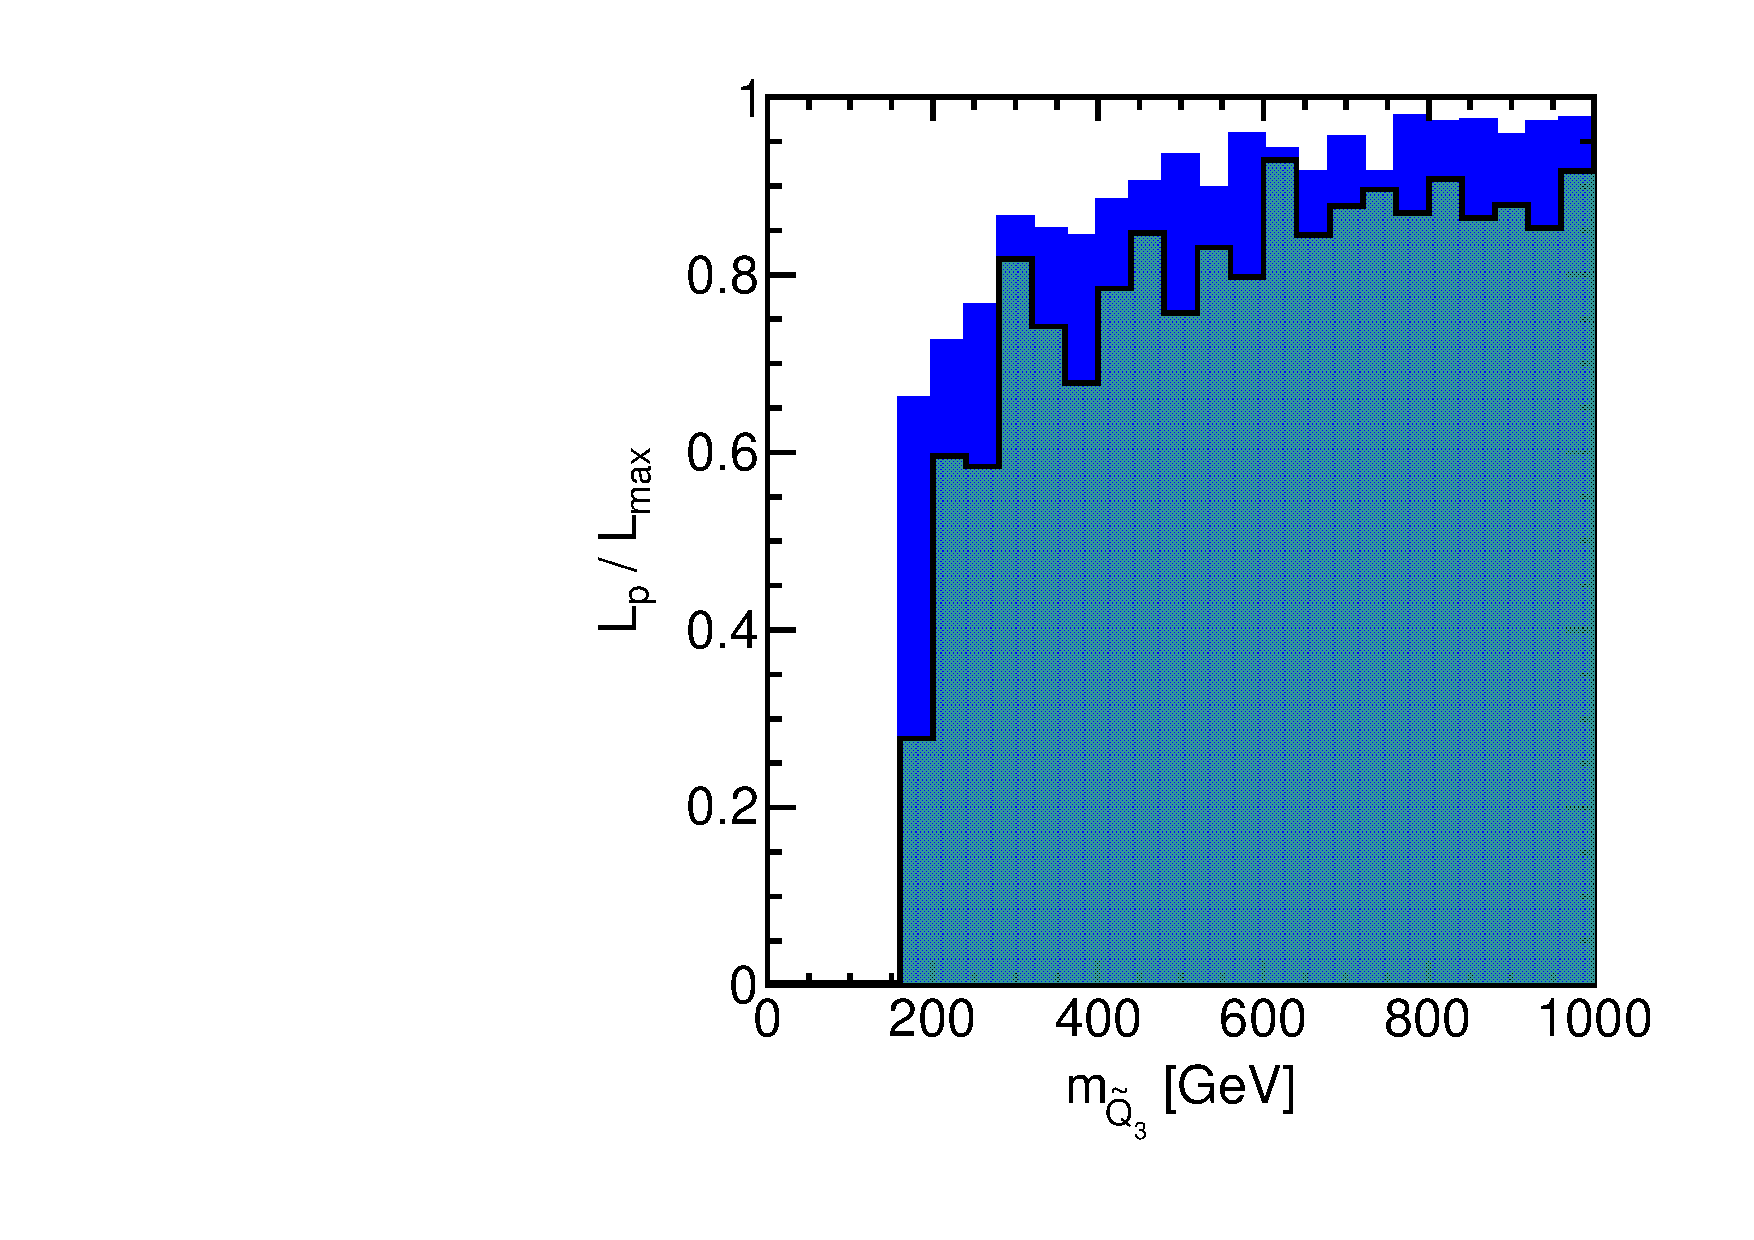
\includegraphics[height=5.5cm]{figs/fig_m_Q_3.pdf} \\
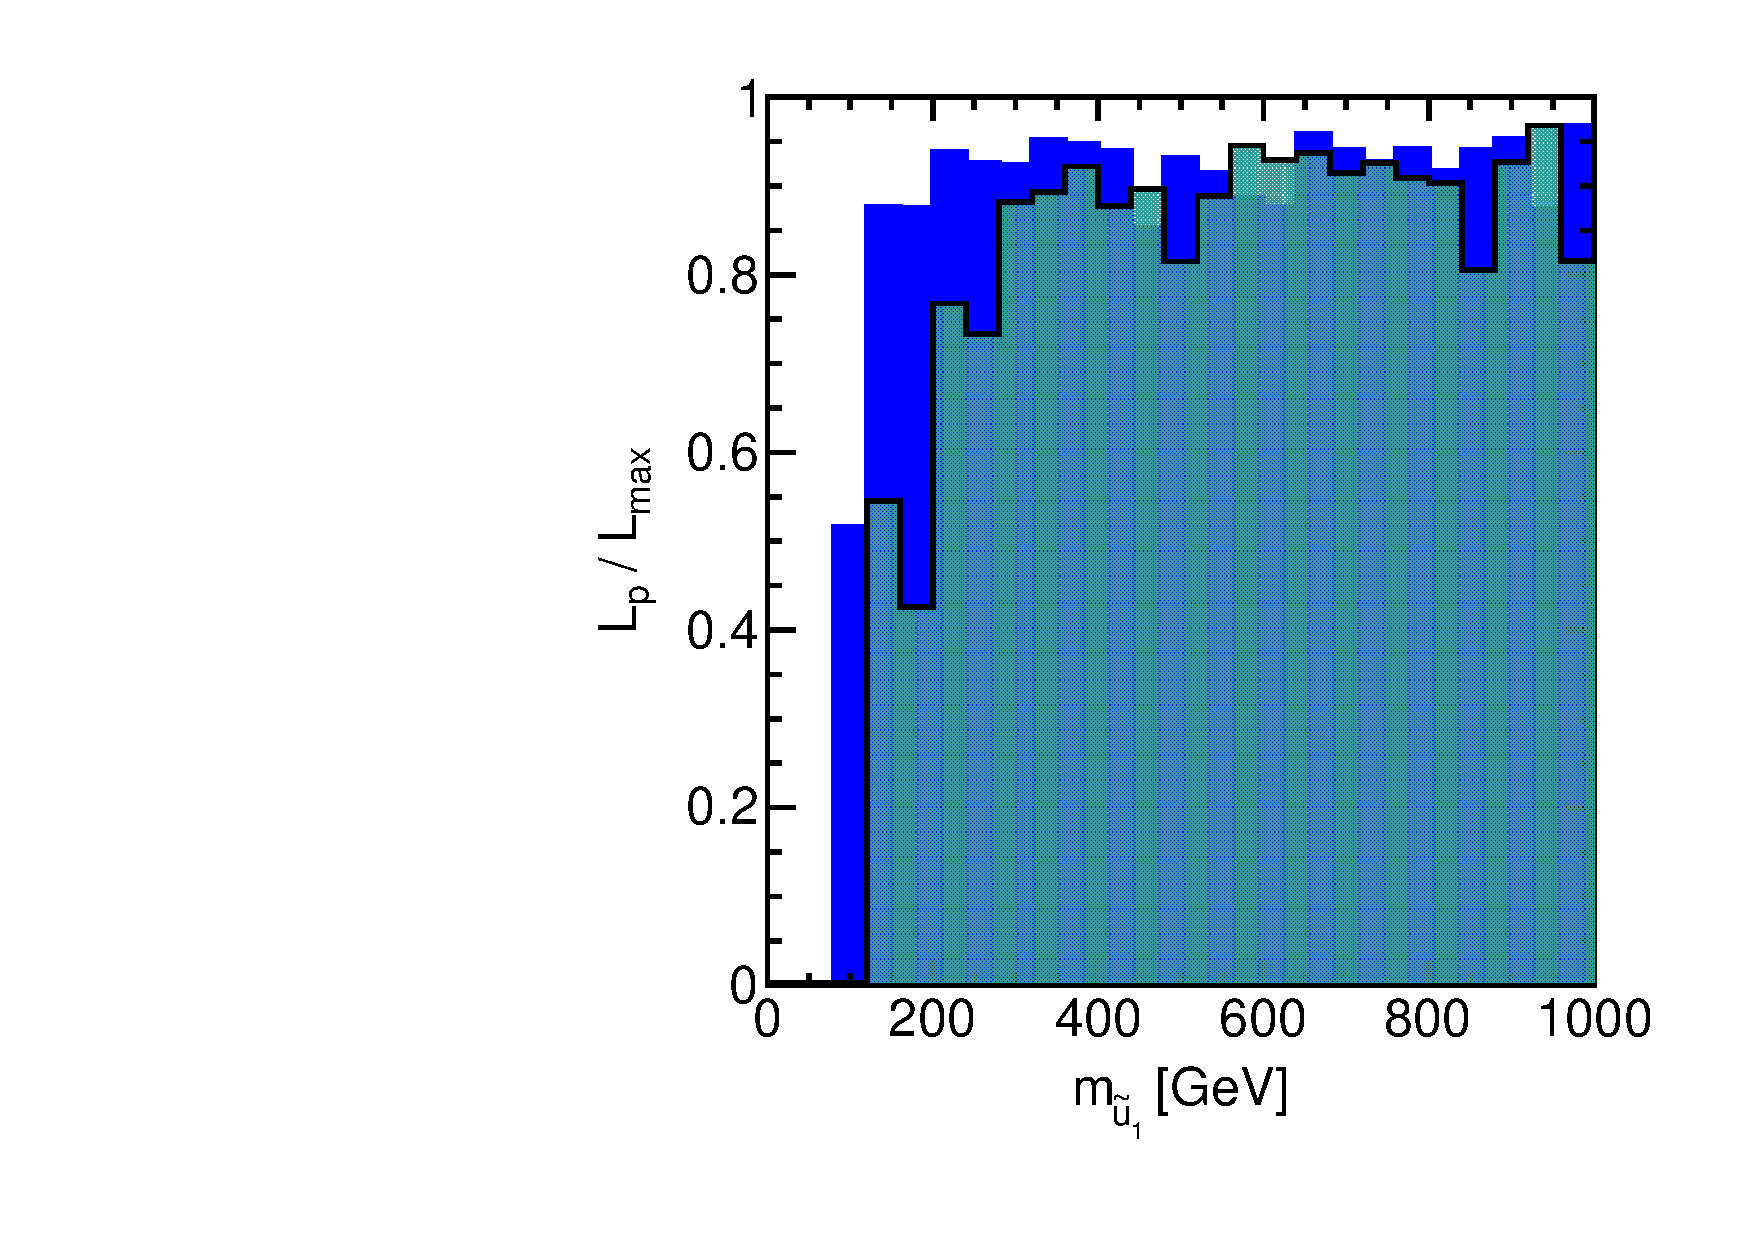
\includegraphics[height=5.5cm]{figs/fig_m_u_1.pdf}
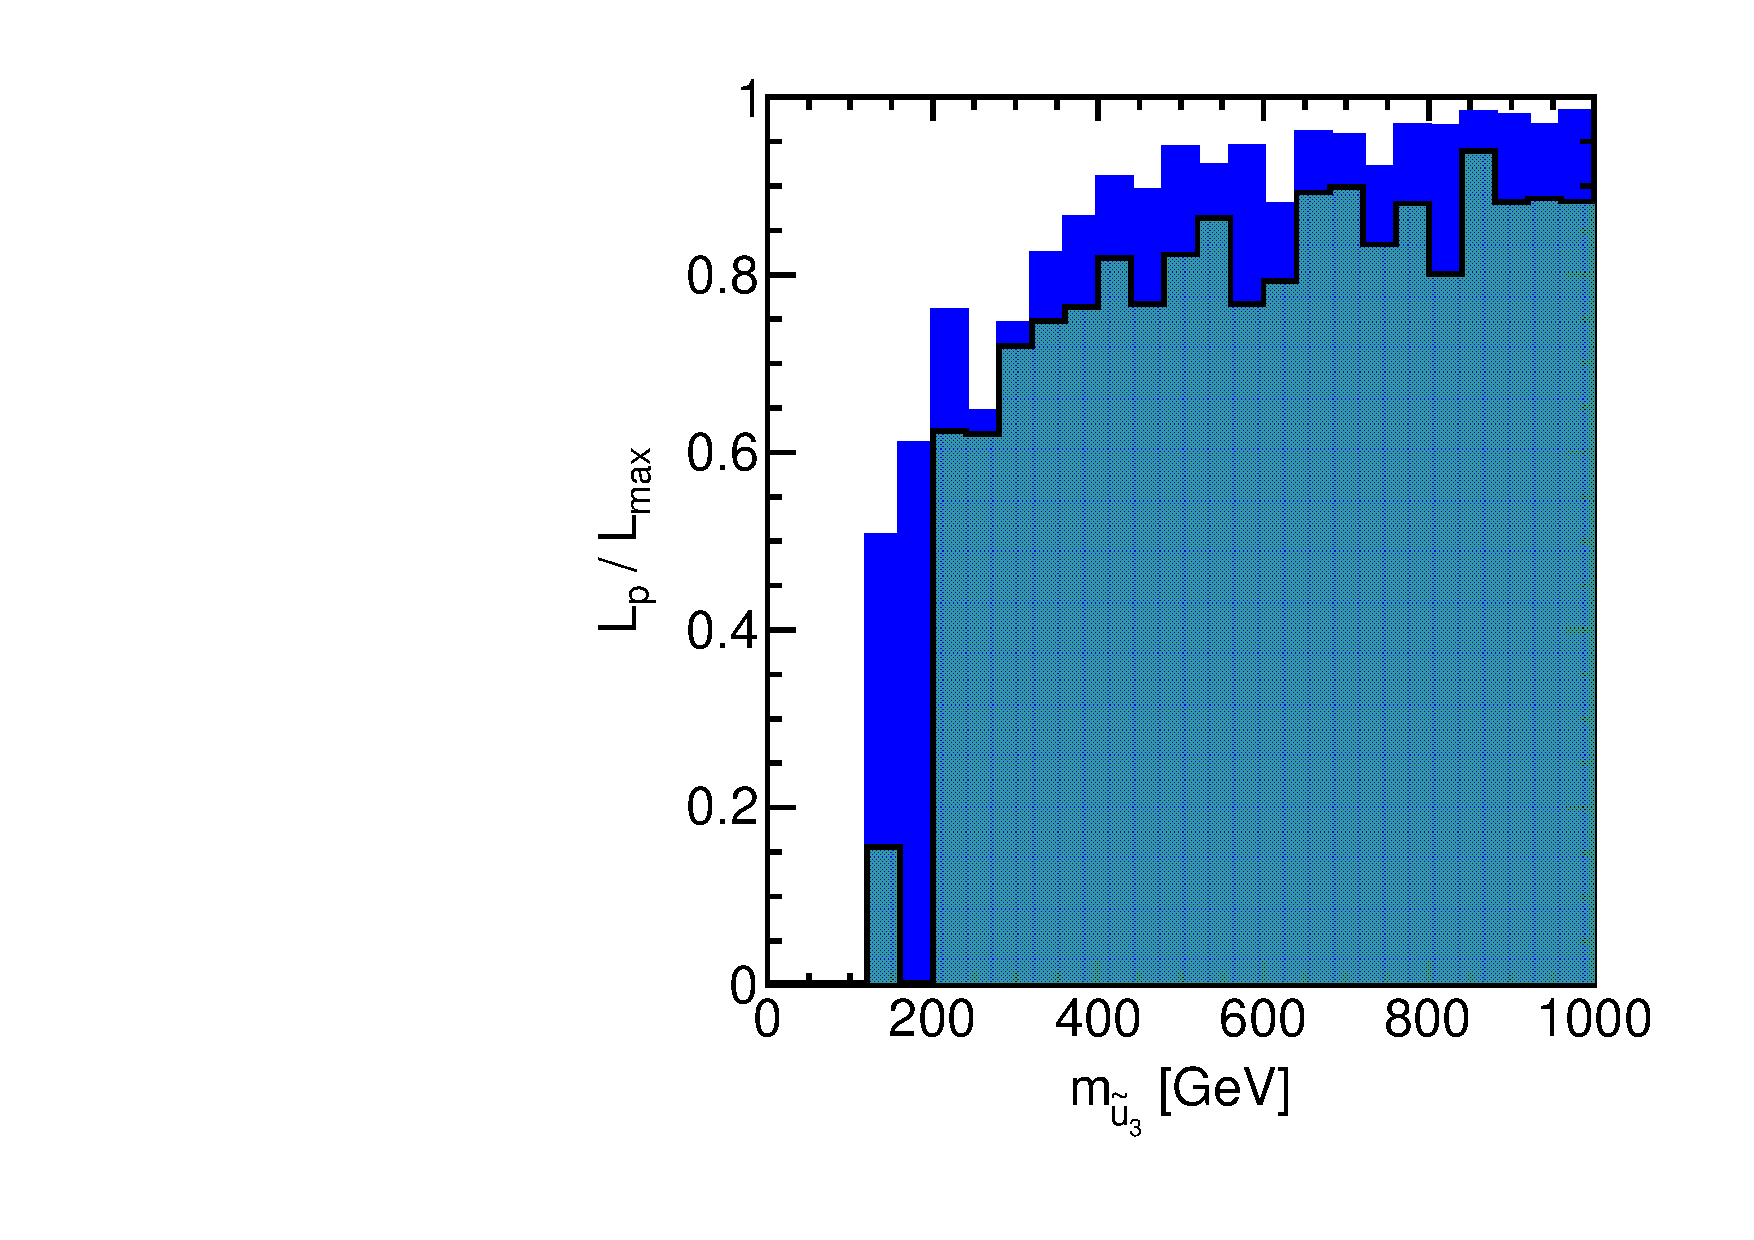
\includegraphics[height=5.5cm]{figs/fig_m_u_3.pdf} \\
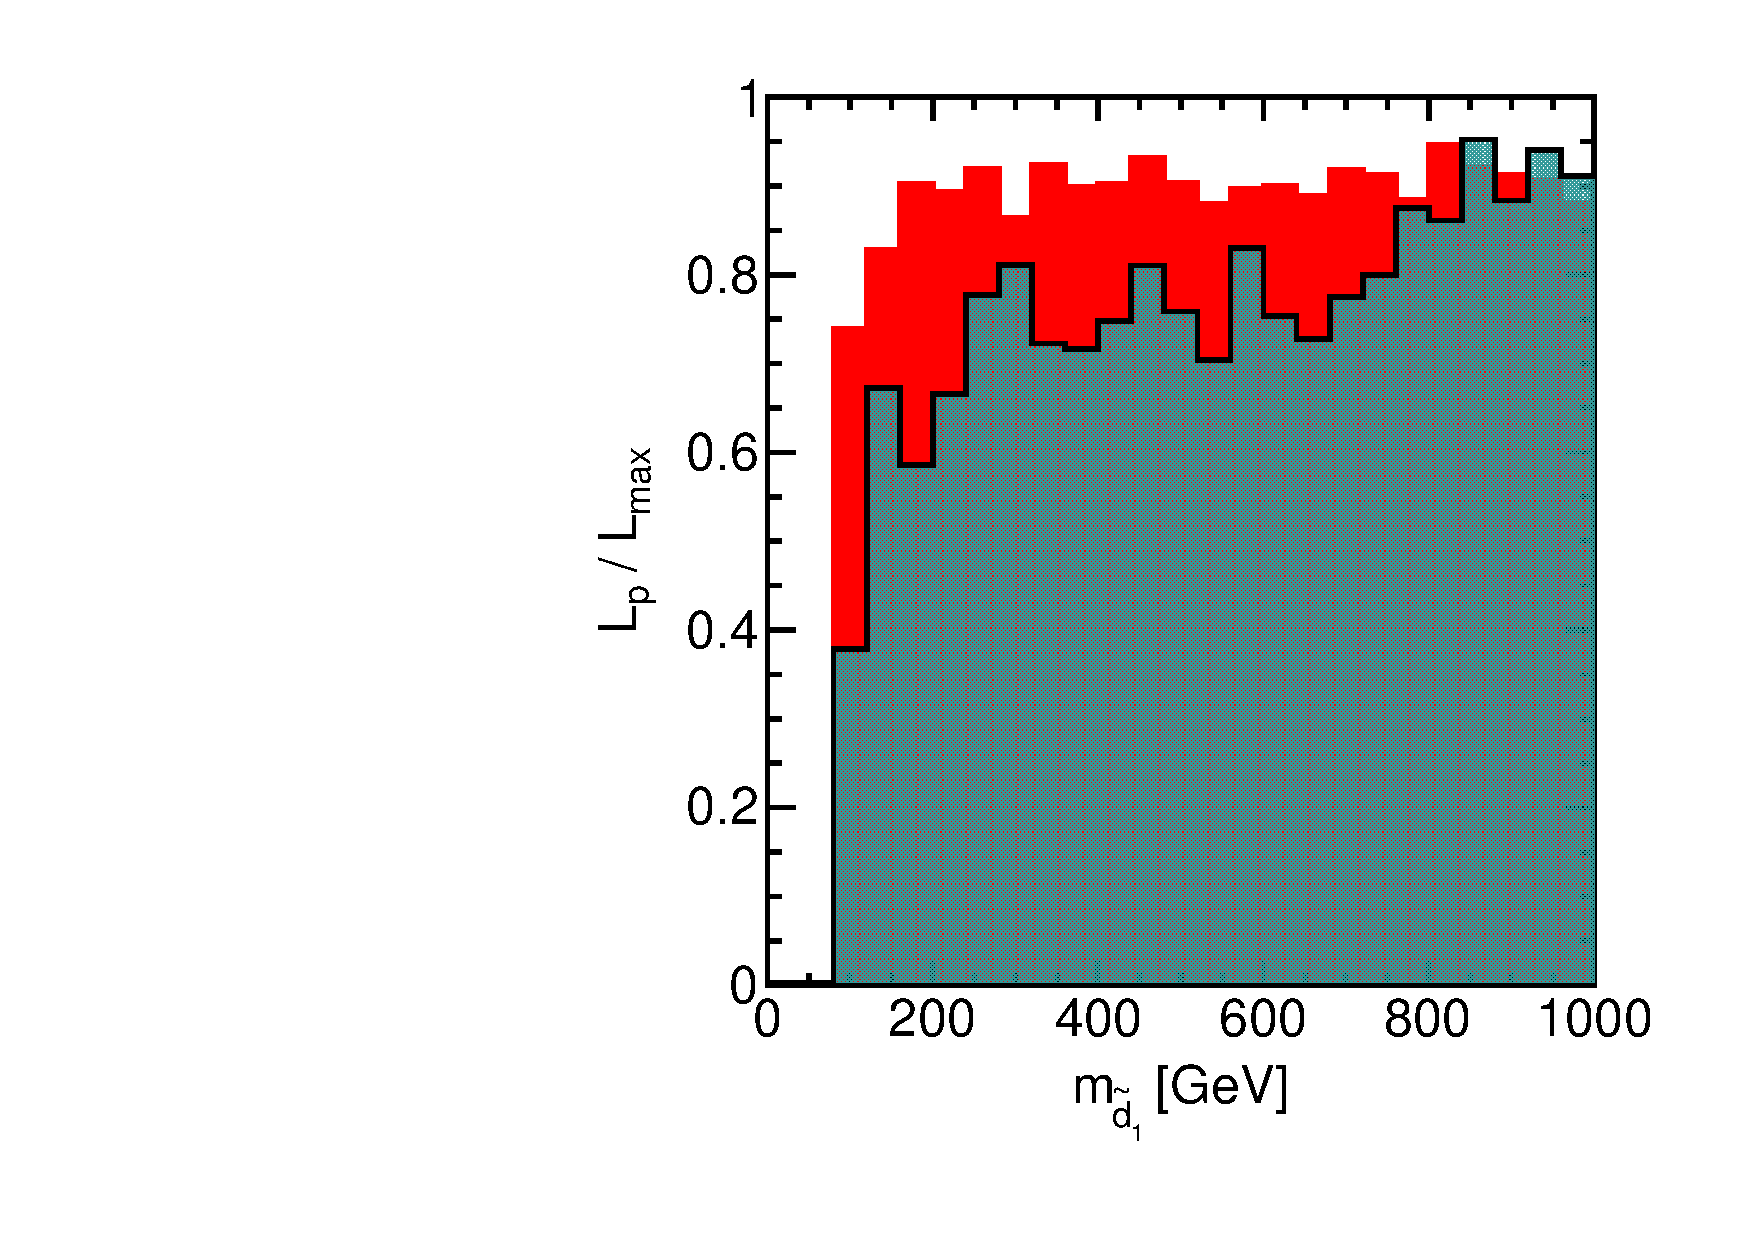
\includegraphics[height=5.5cm]{figs/fig_m_d_1.pdf}
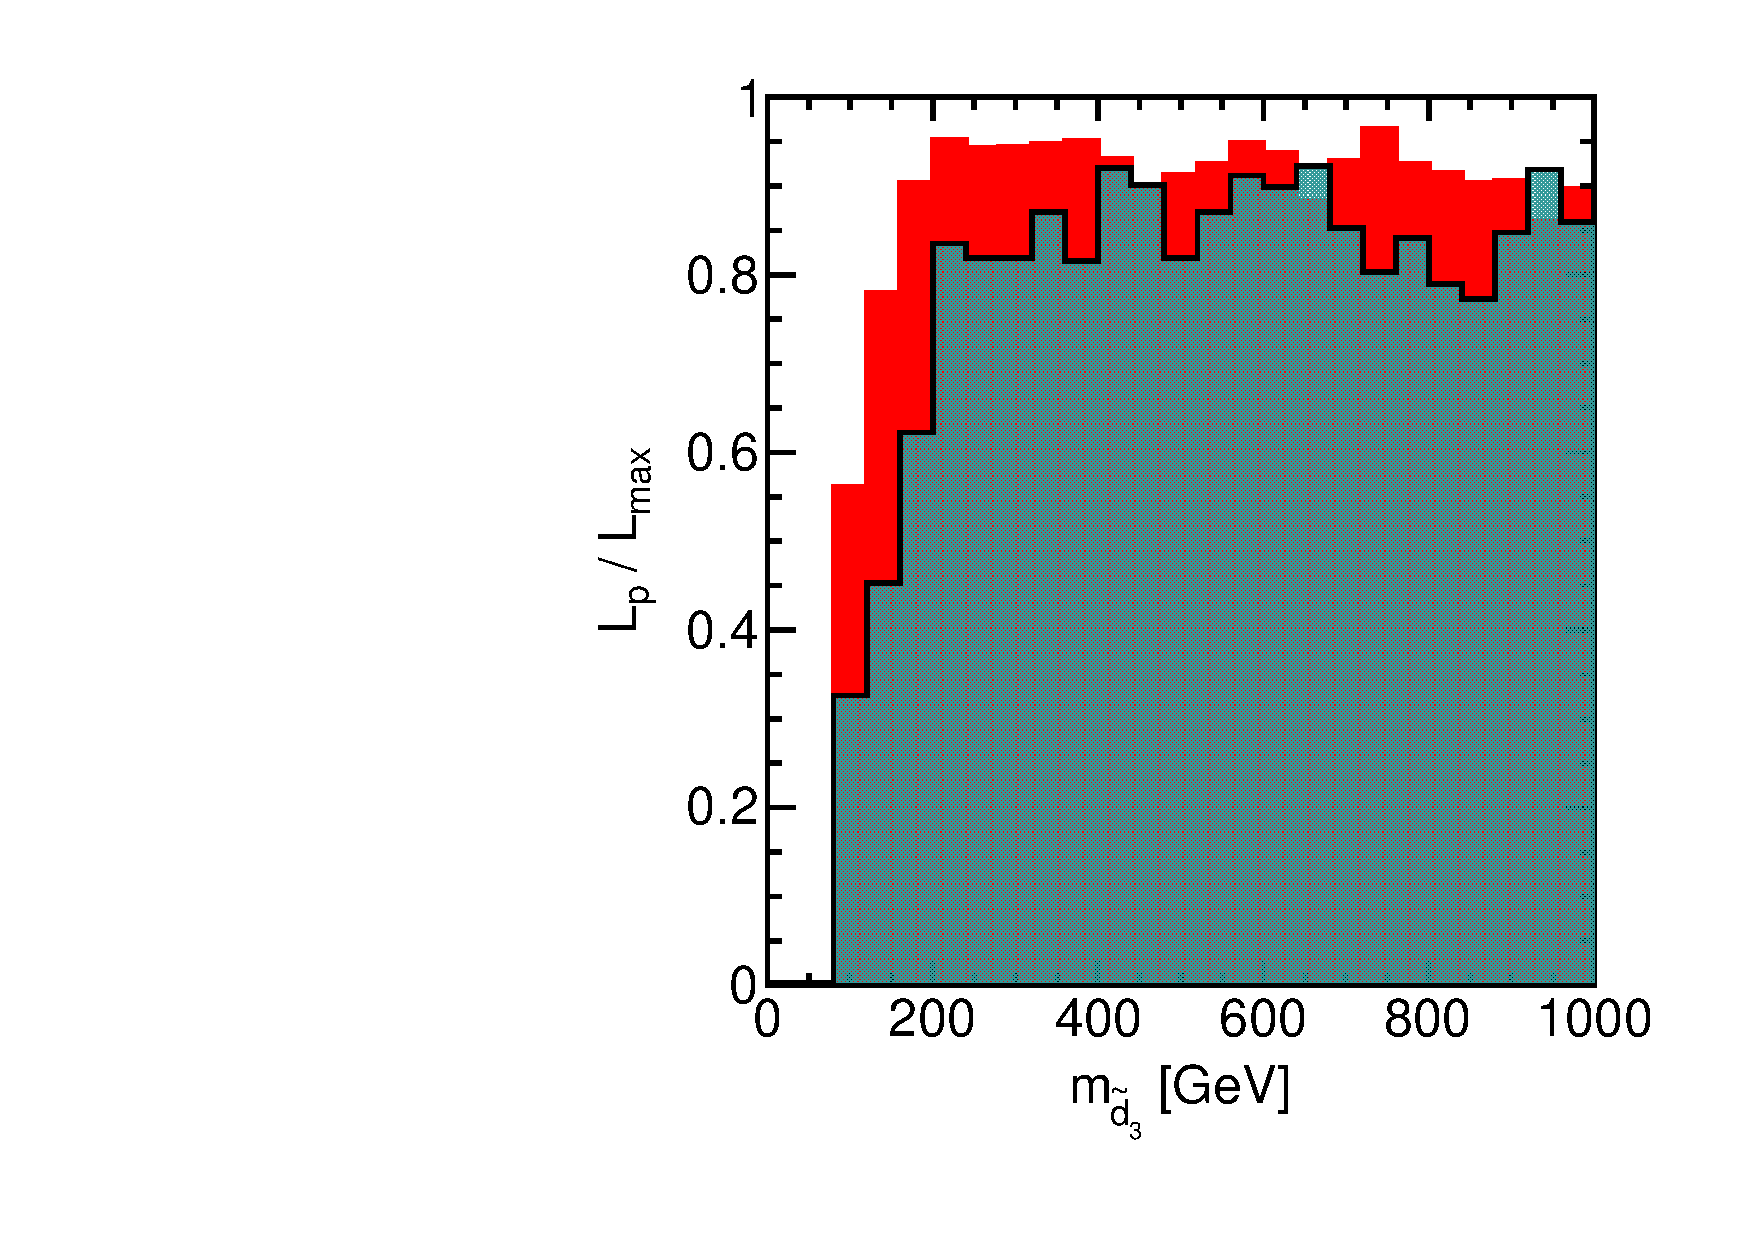
\includegraphics[height=5.5cm]{figs/fig_m_d_3.pdf}
\caption{Ratios of profile likelihood $L_p$ to maximum likelihood $L_{max}$ shown for the squark mass parameters at SUSY scale.  The colored and shaded histograms show the distributions before and after the inclusion of the CMS results.}
\label{fig:LRwcms_msq}
\end{center}
\end{figure}


\begin{figure}[htbp]
\begin{center}
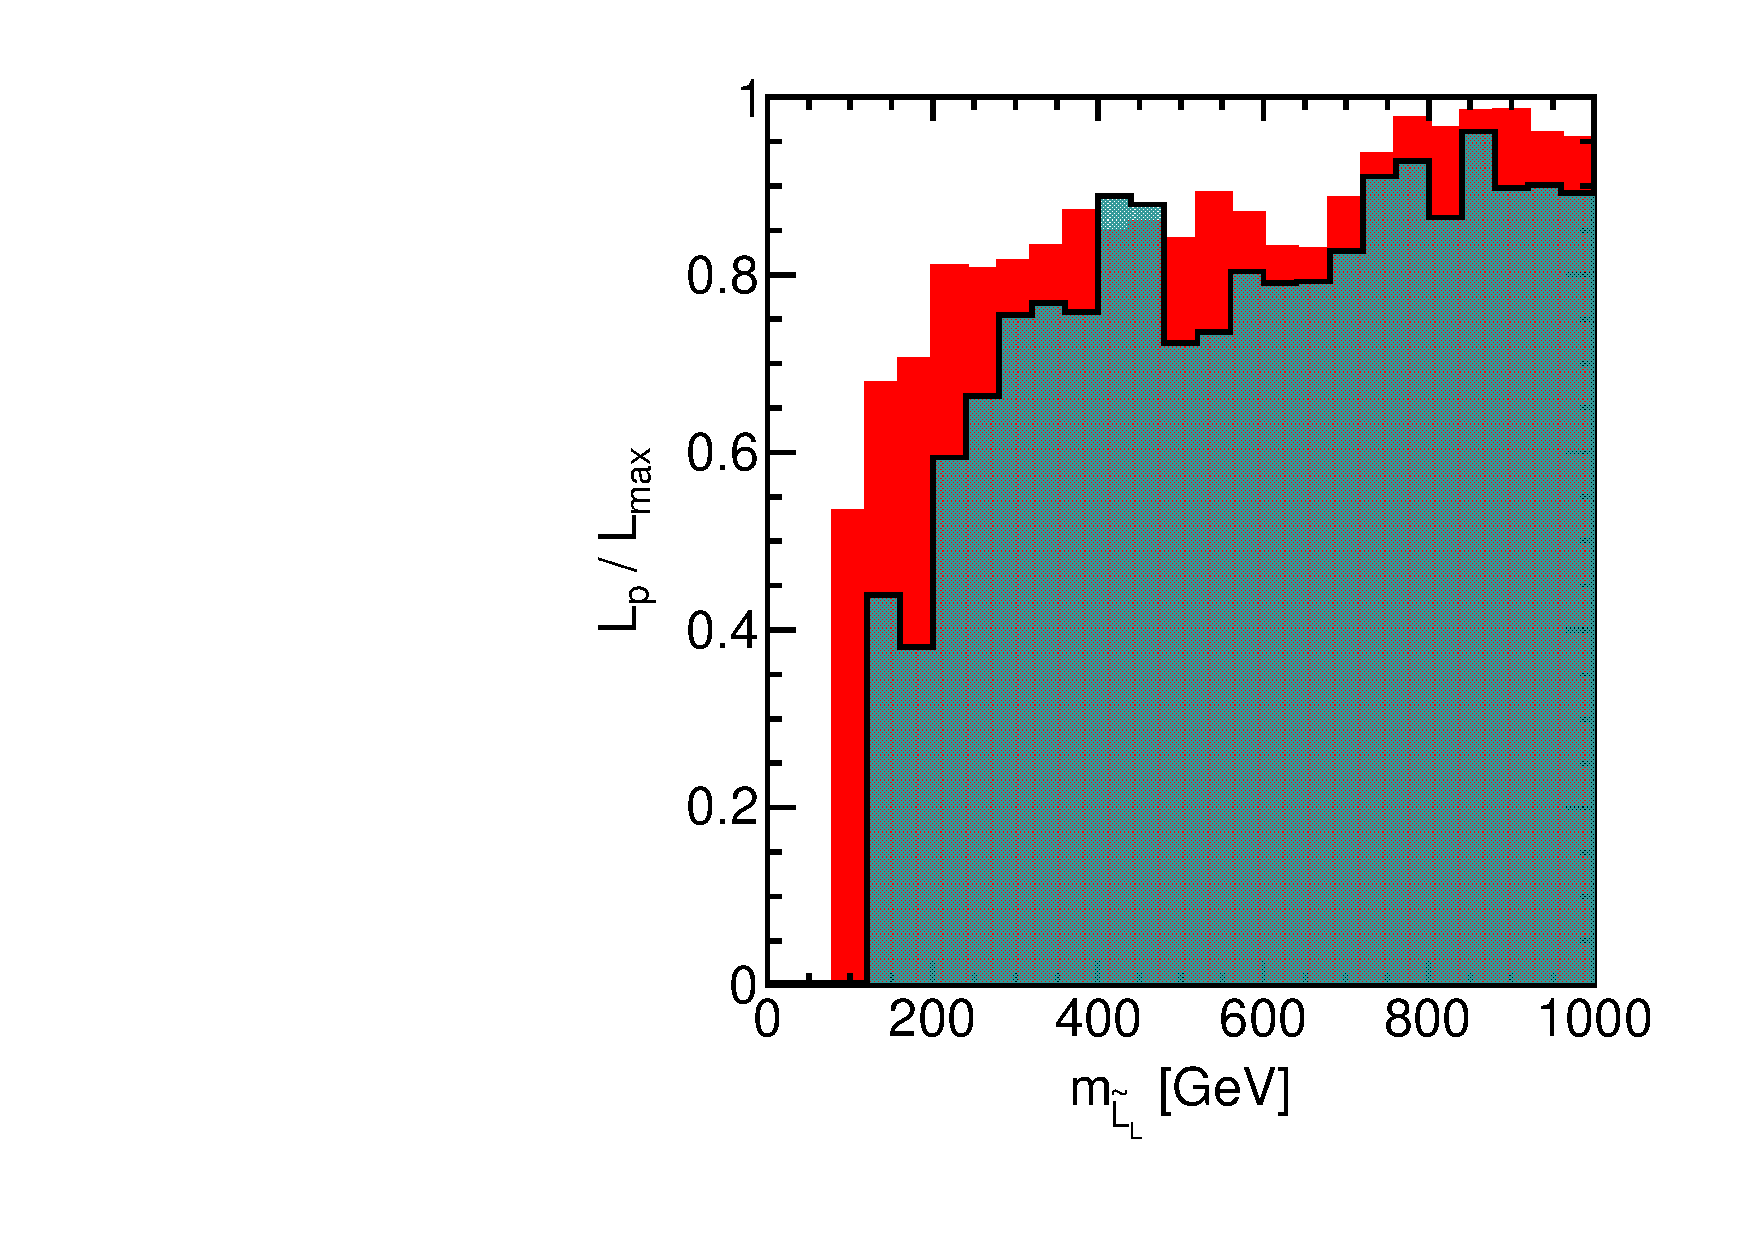
\includegraphics[height=5.5cm]{figs/fig_m_L_L.pdf} 
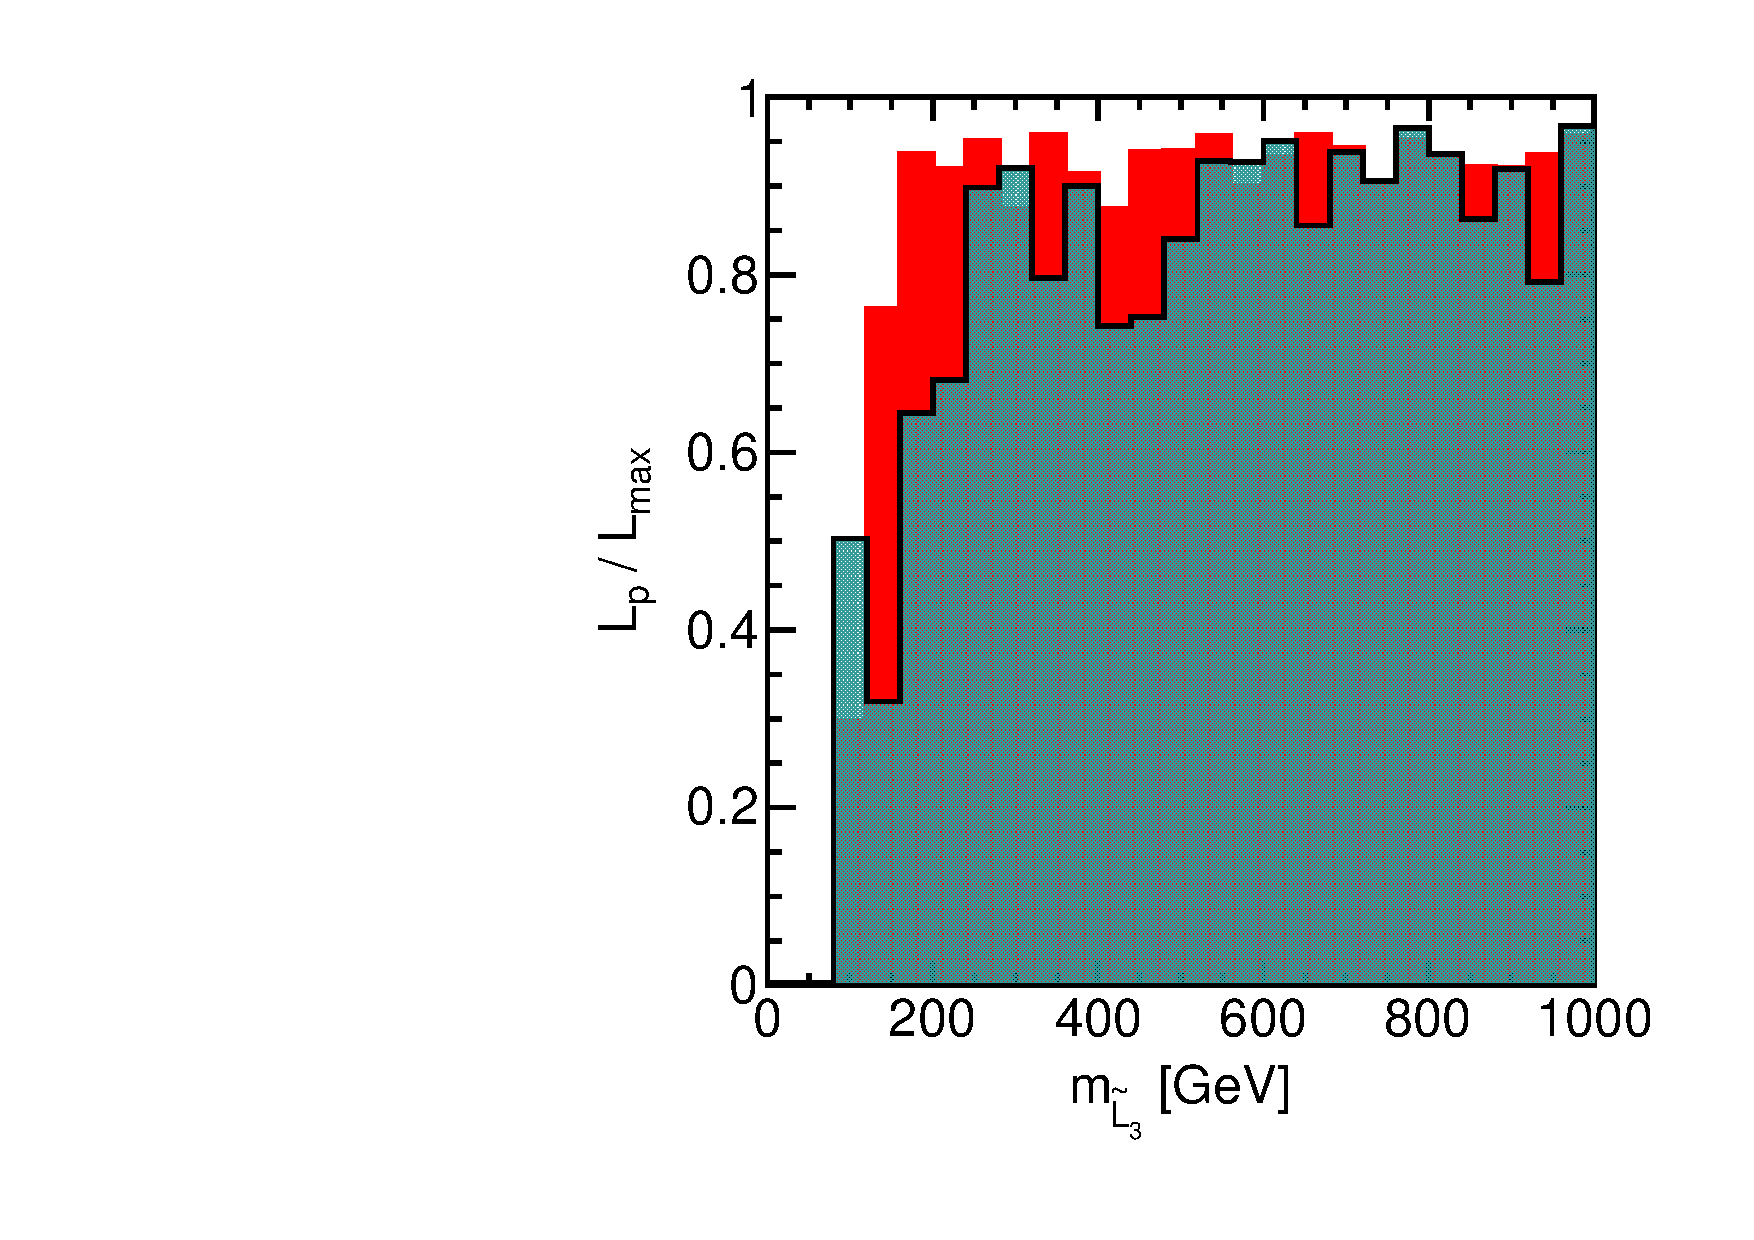
\includegraphics[height=5.5cm]{figs/fig_m_L_3.pdf} \\
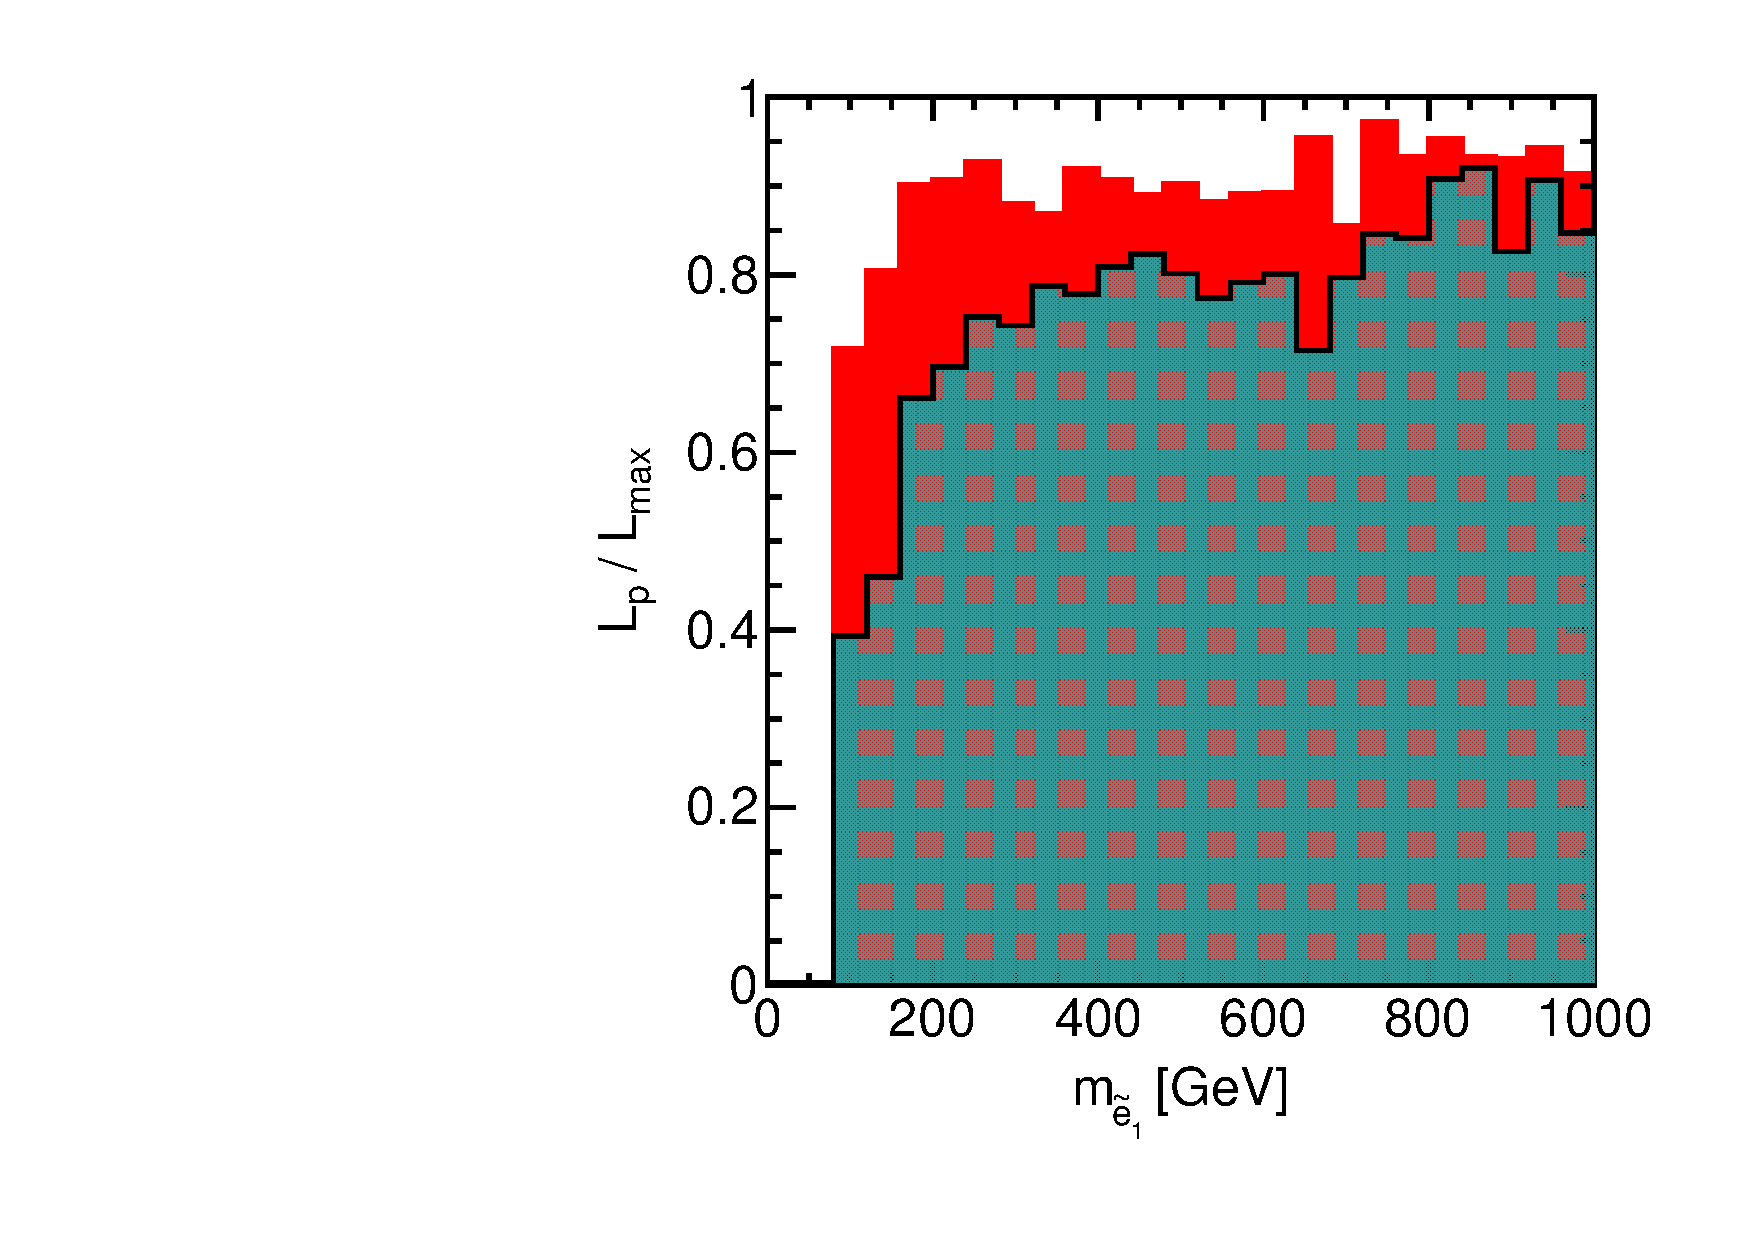
\includegraphics[height=5.5cm]{figs/fig_m_e_1.pdf}
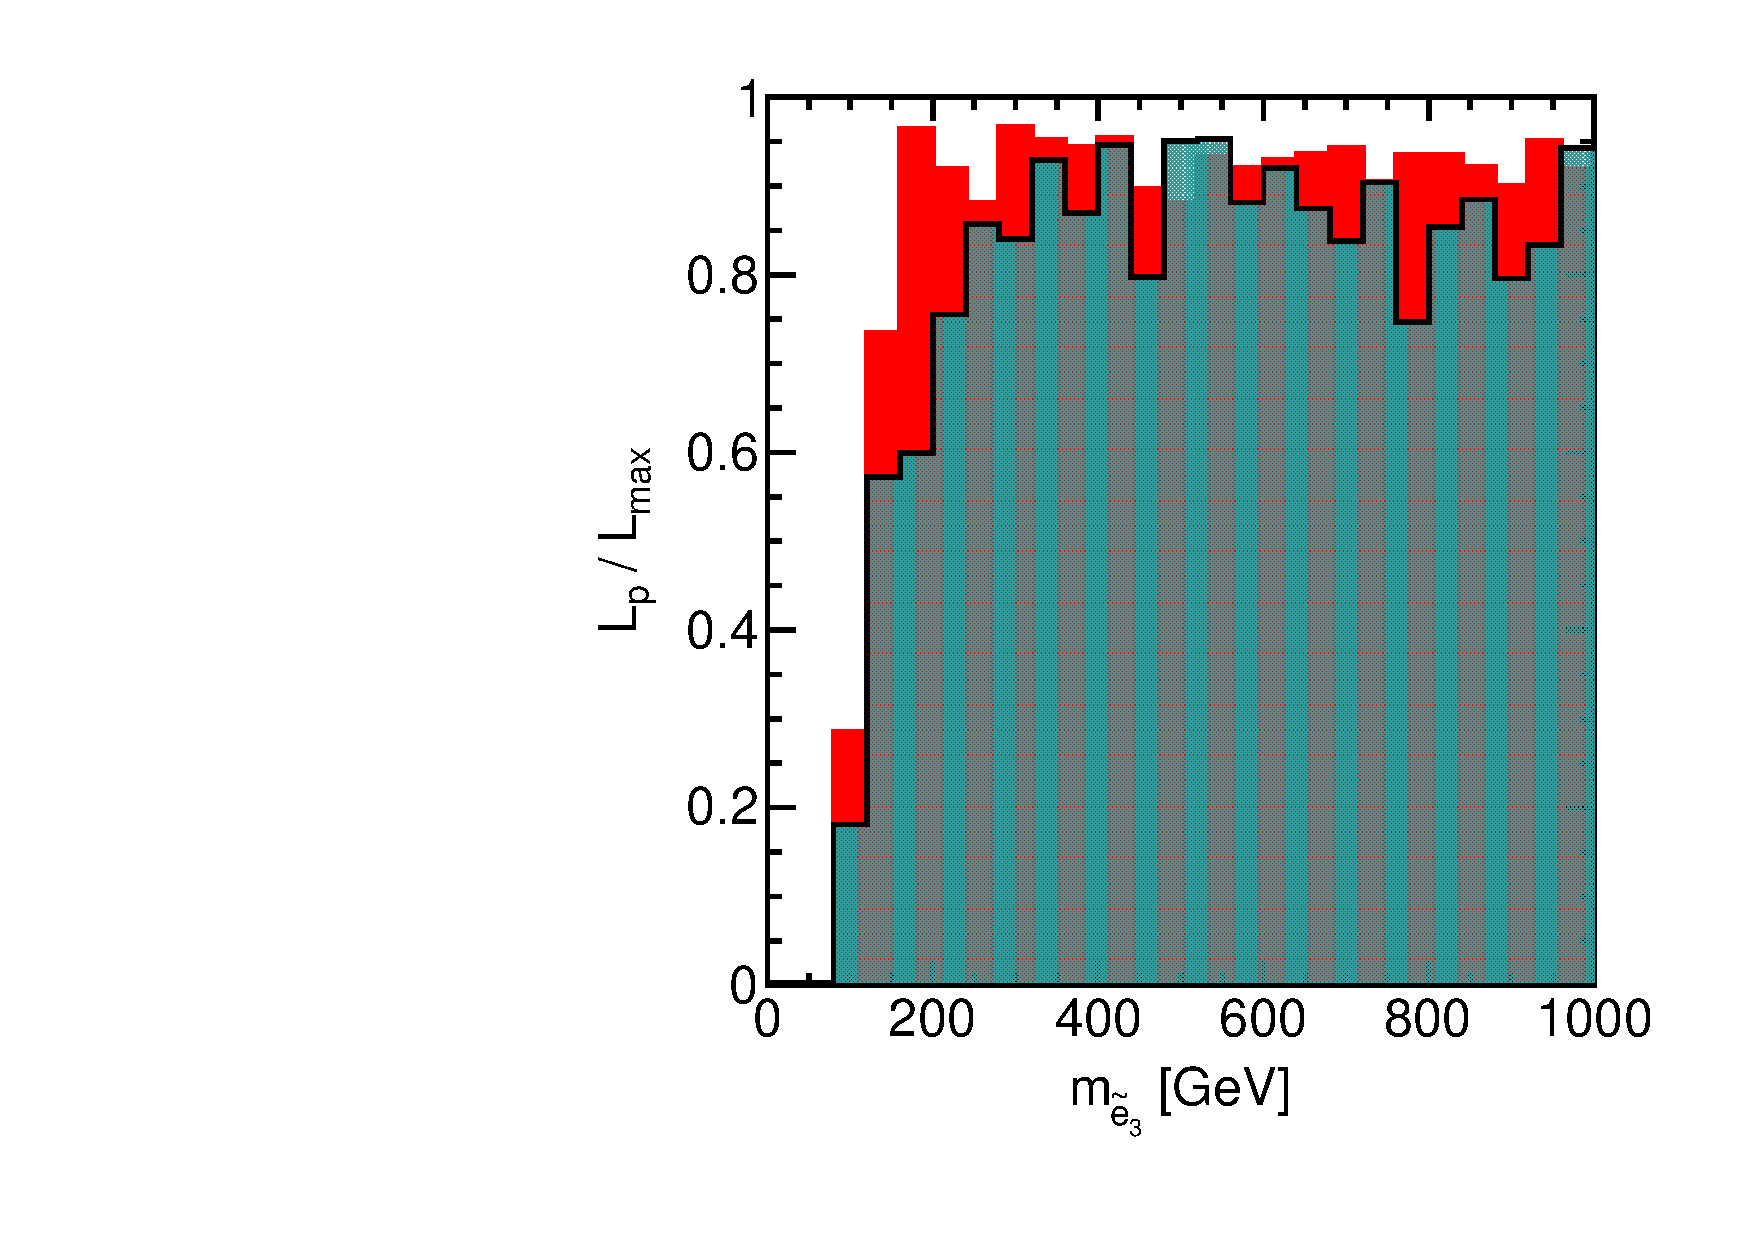
\includegraphics[height=5.5cm]{figs/fig_m_e_3.pdf}
\caption{Ratios of profile likelihood $L_p$ to maximum likelihood $L_{max}$ shown for the slepton mass parameters at SUSY scale.  The colored and shaded histograms show the distributions before and after the inclusion of the CMS results.}
\label{fig:LRwcms_msl}
\end{center}
\end{figure}


\begin{figure}[htbp]
\begin{center}
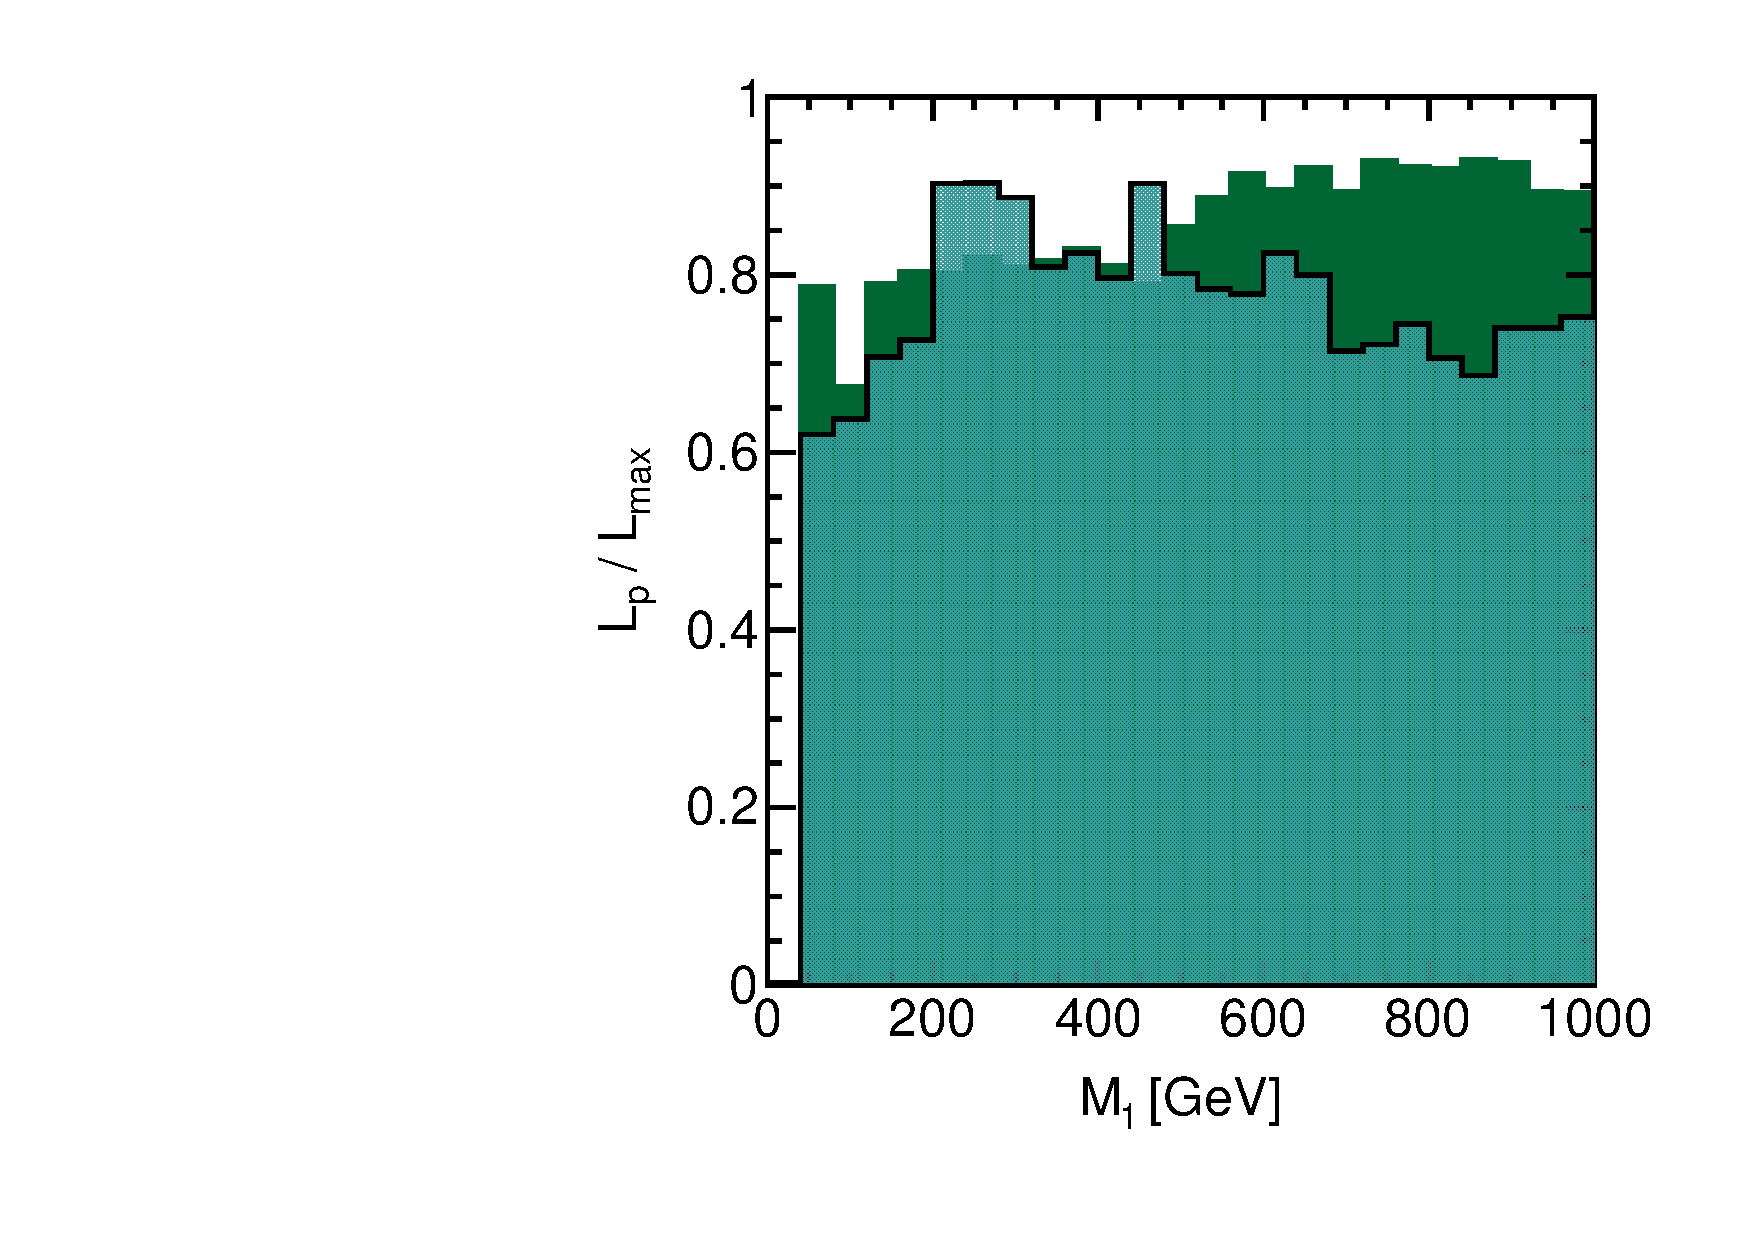
\includegraphics[height=5.5cm]{figs/fig_M_1.pdf} 
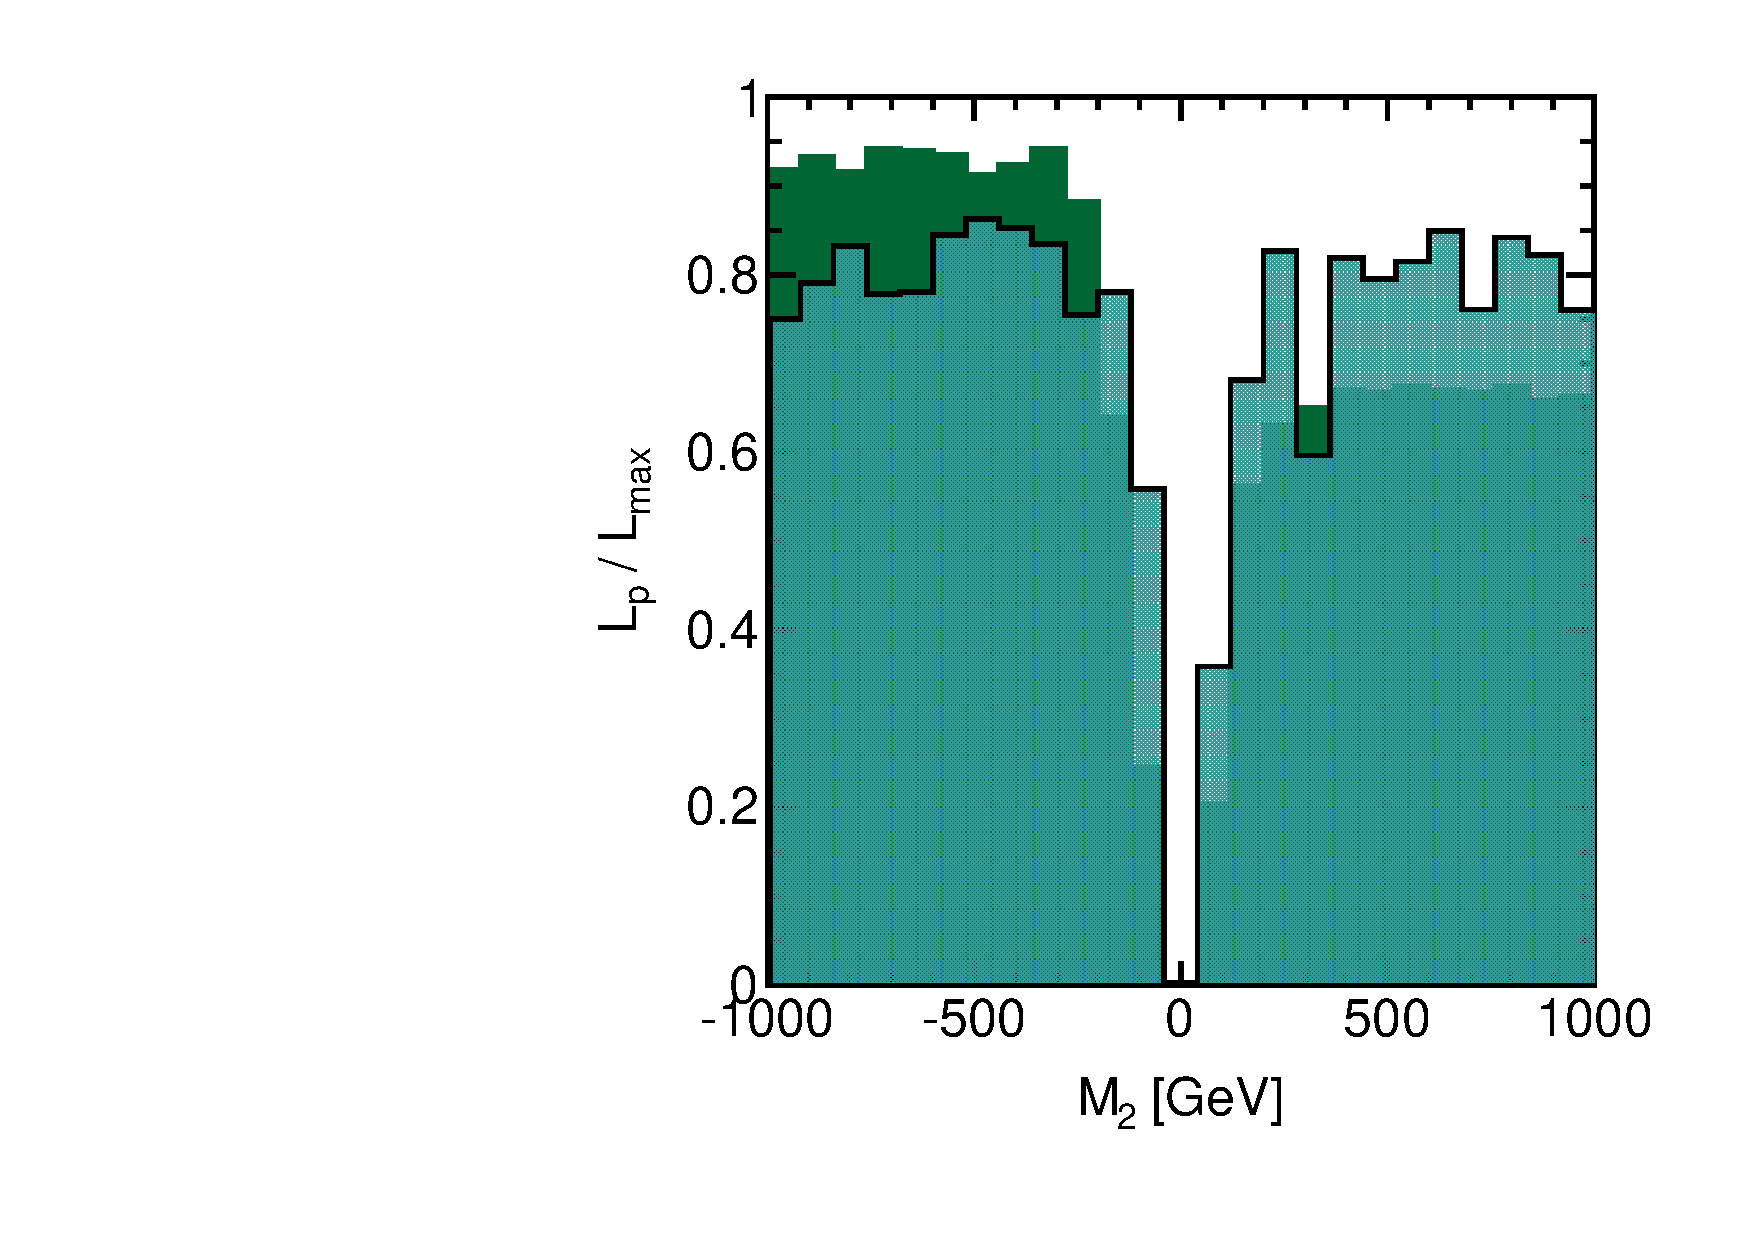
\includegraphics[height=5.5cm]{figs/fig_M_2.pdf} \\
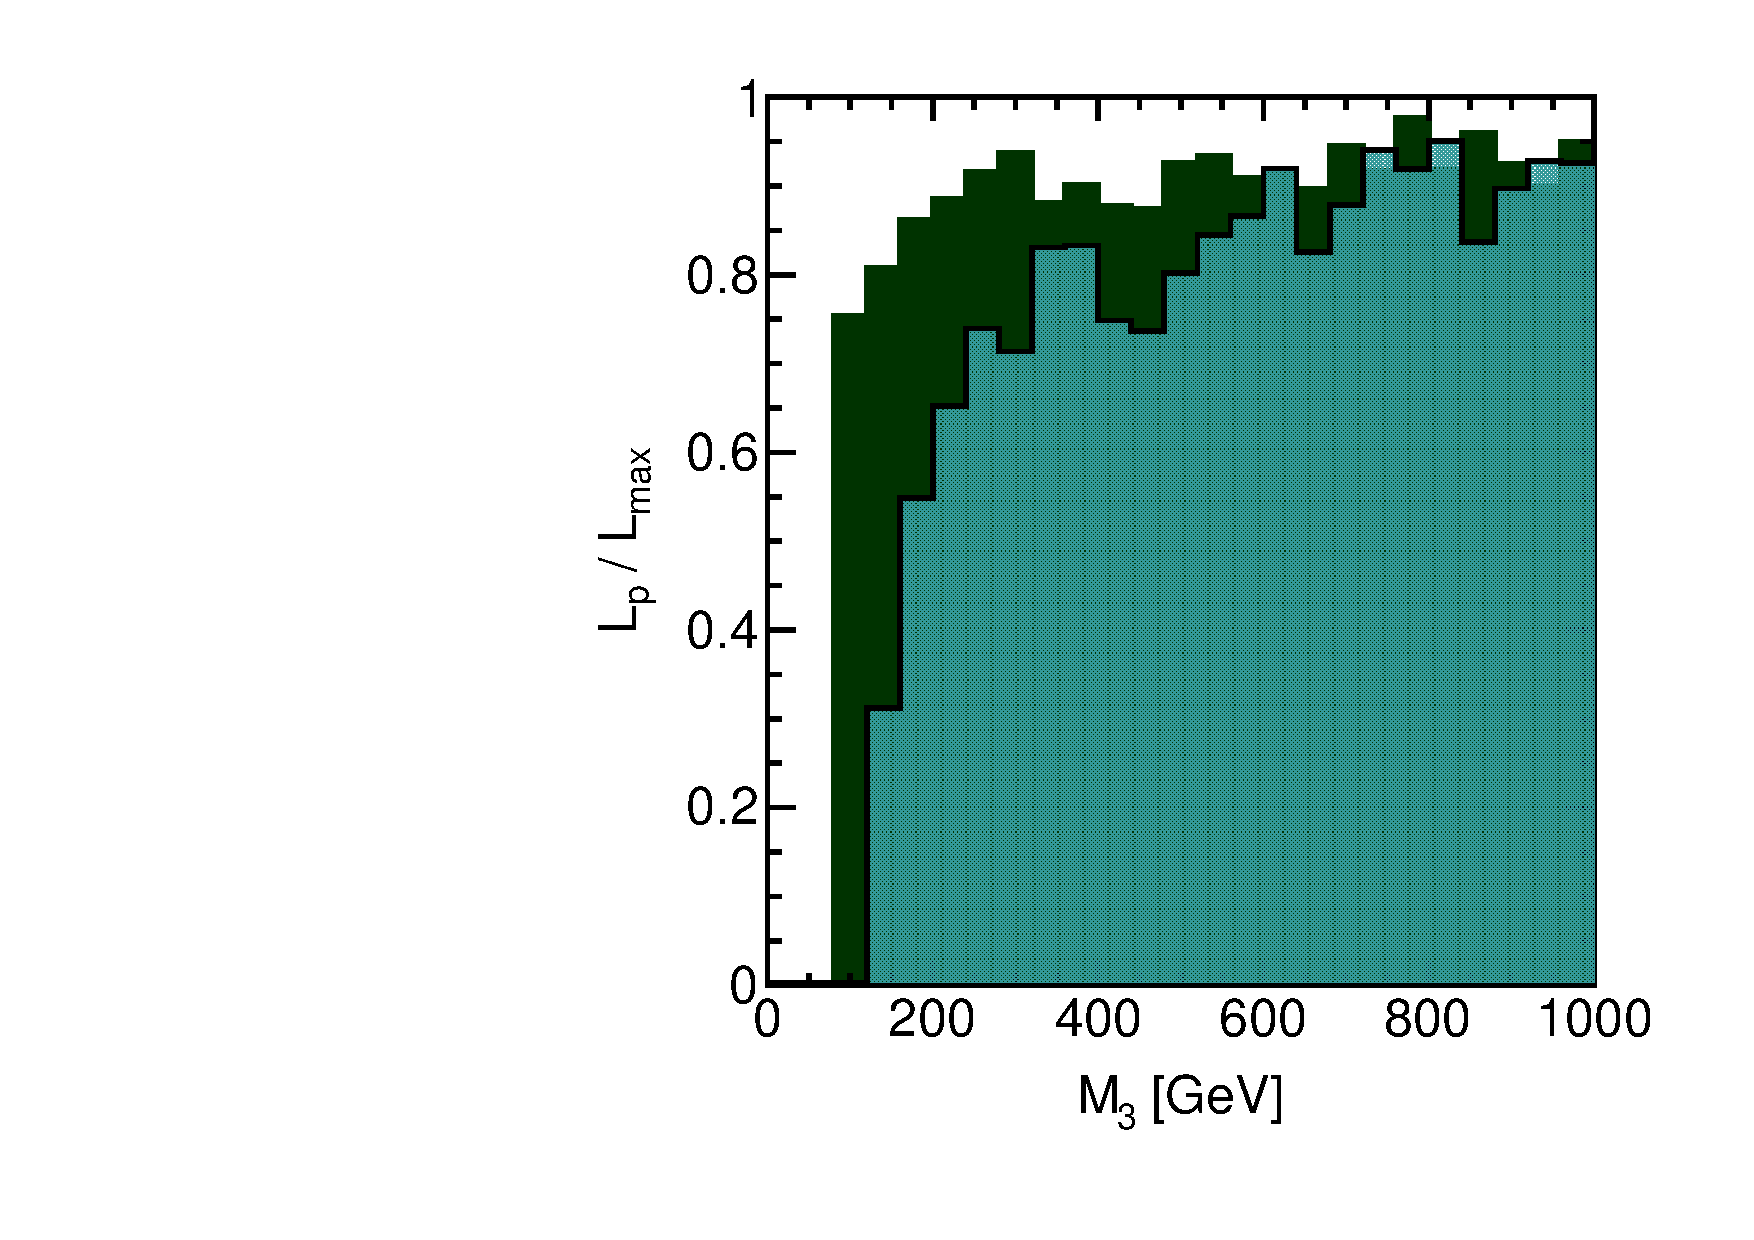
\includegraphics[height=5.5cm]{figs/fig_M_3.pdf}
\caption{Ratios of profile likelihood $L_p$ to maximum likelihood $L_{max}$ shown for gaugino mass parameters at  SUSY scale.  The colored and shaded histograms show the distributions before and after the inclusion of the CMS results.}
\label{fig:LRwcms_M}
\end{center}
\end{figure}


\begin{figure}[htbp]
\begin{center}
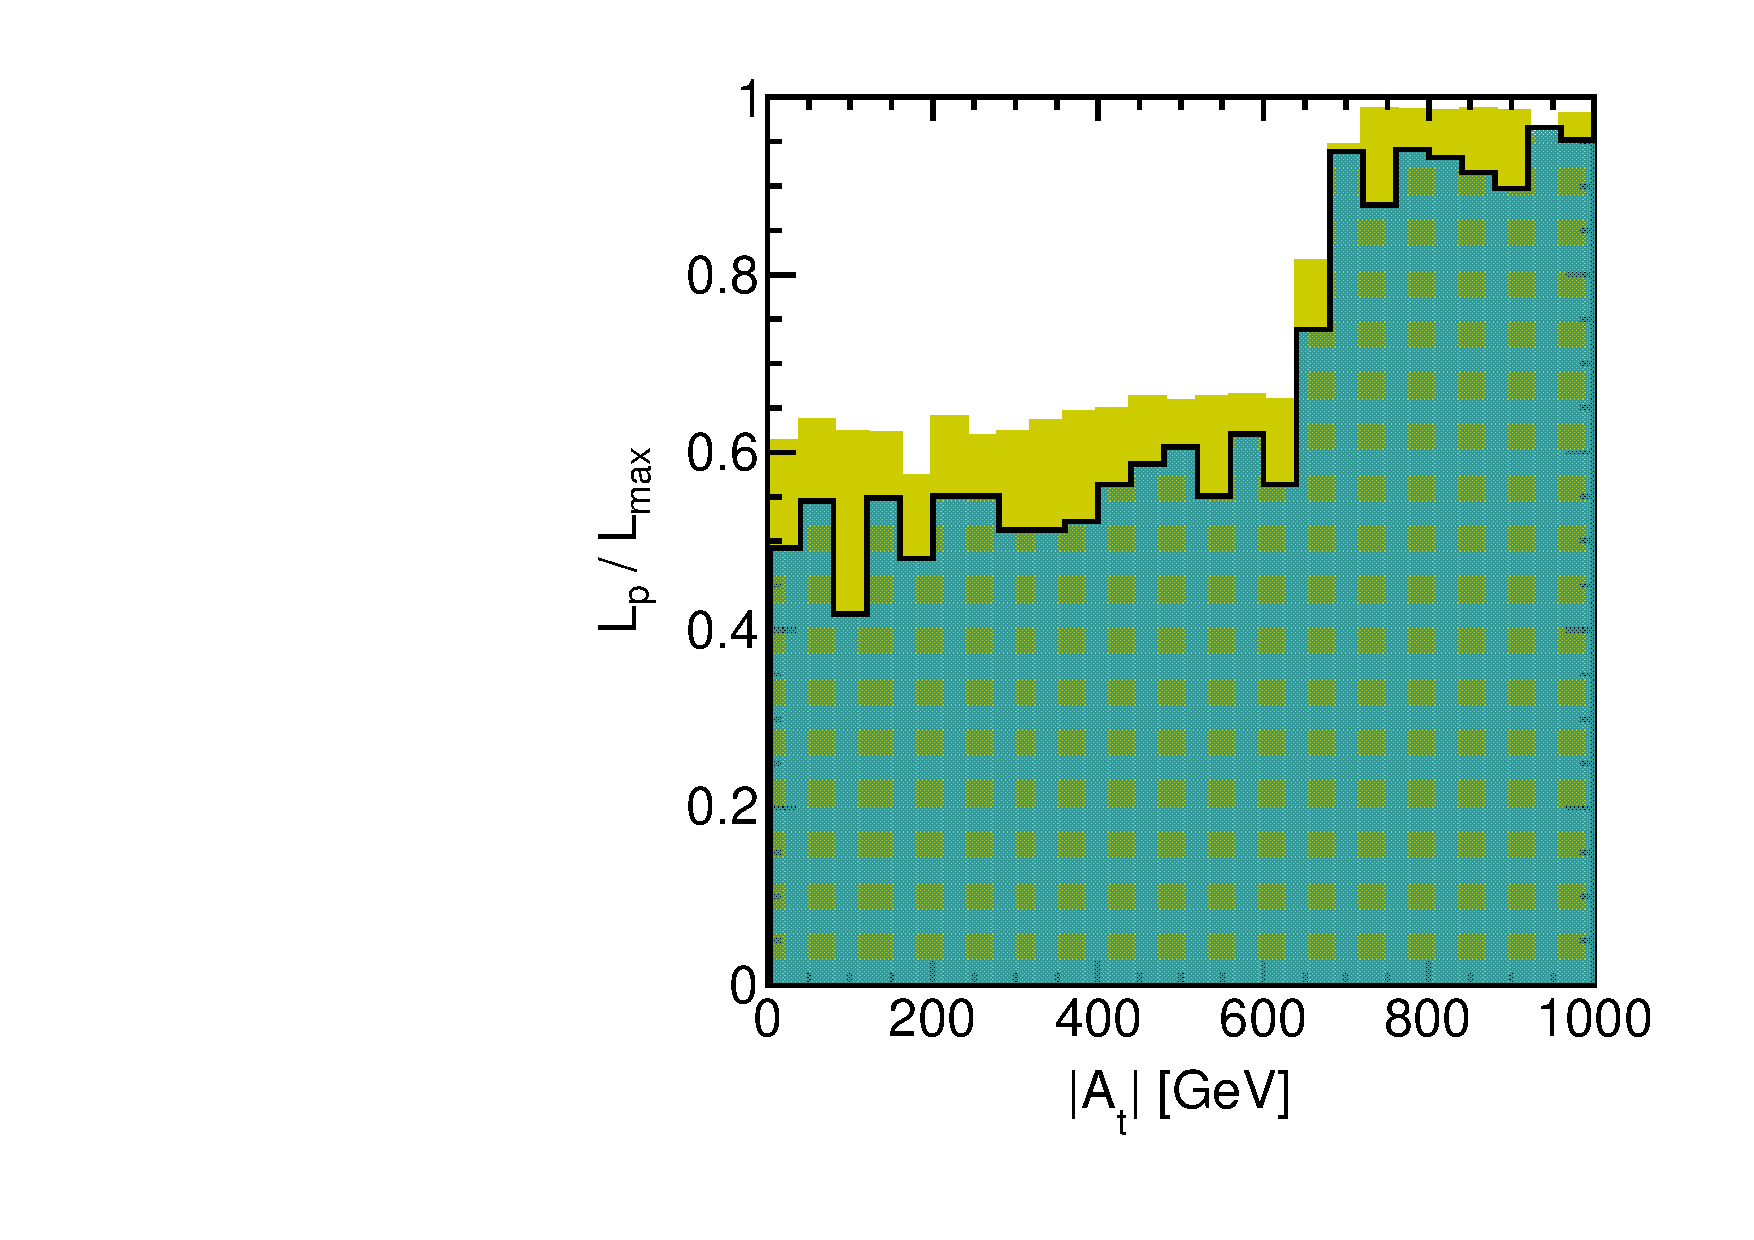
\includegraphics[height=5.5cm]{figs/fig_A_t.pdf} 
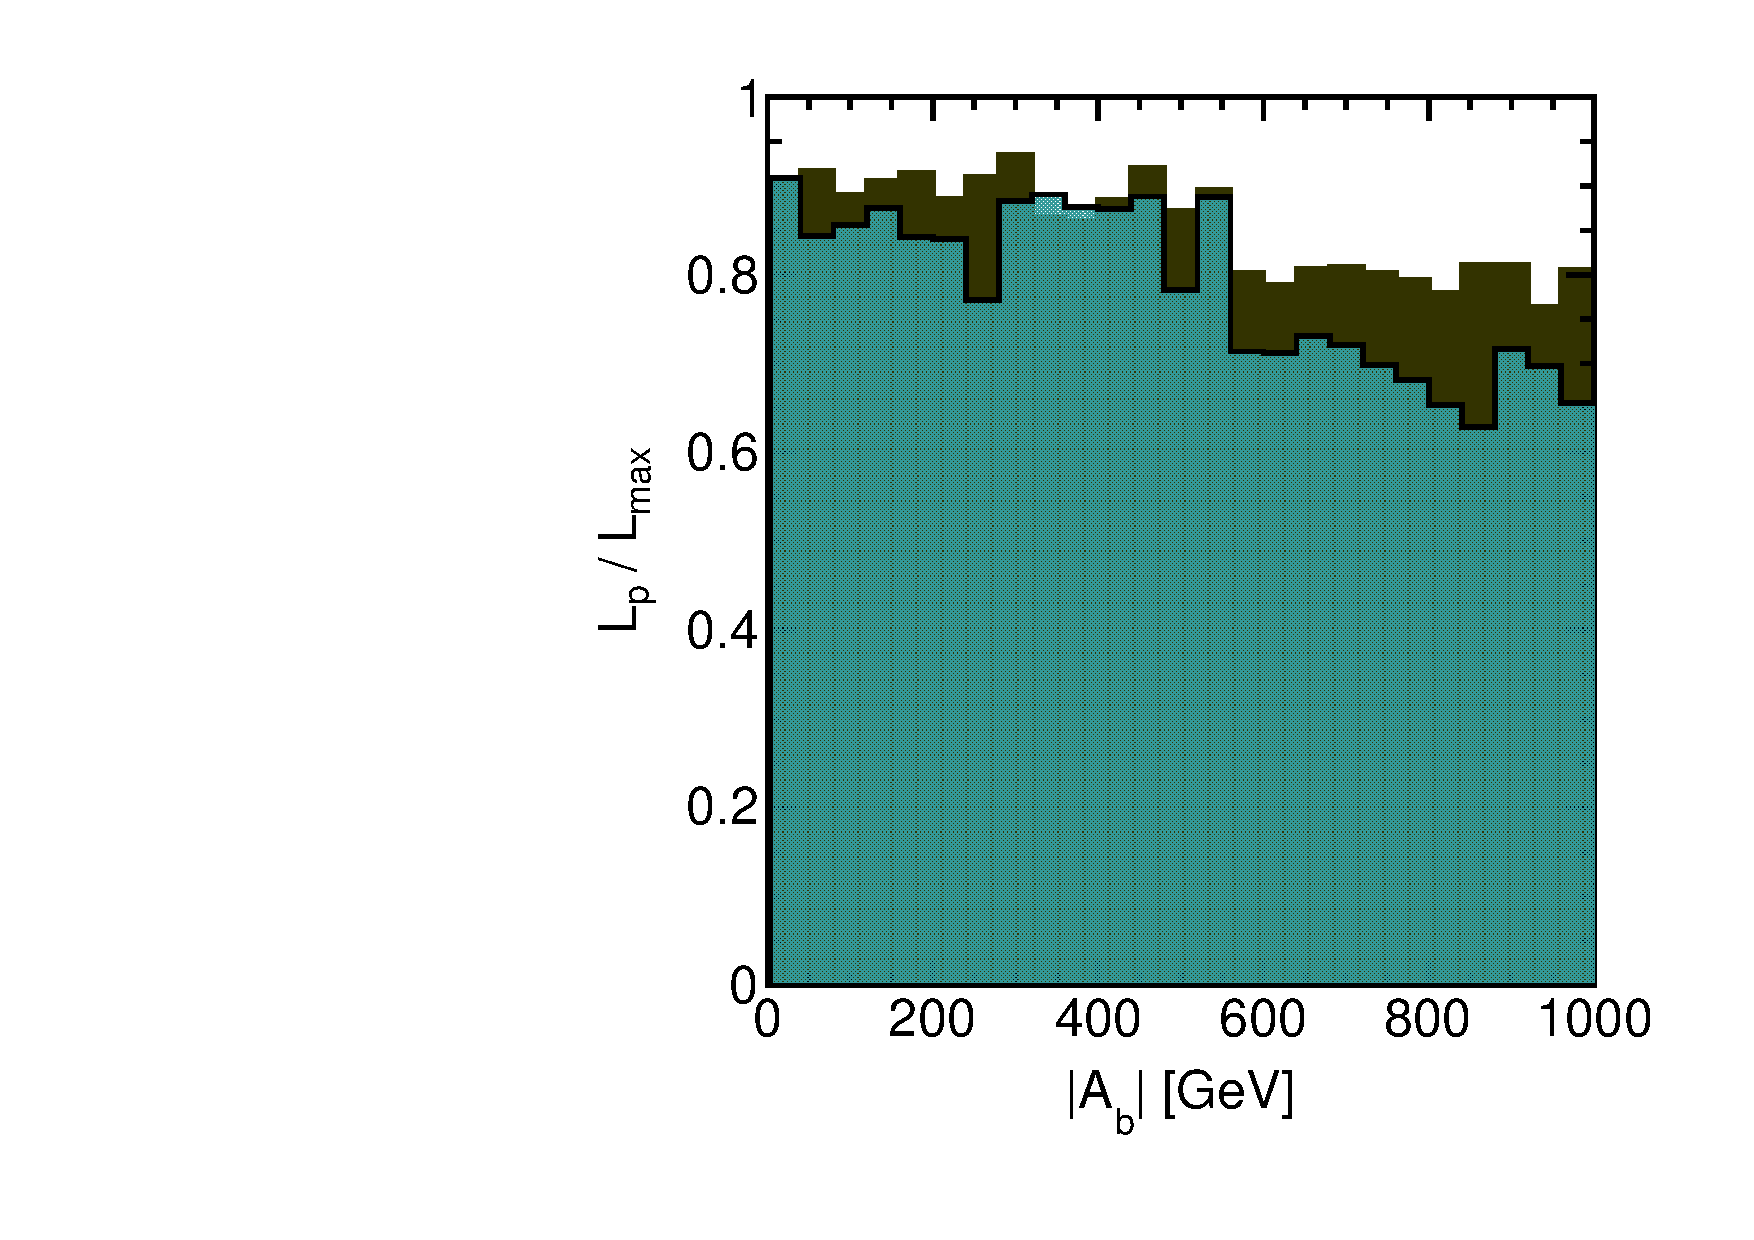
\includegraphics[height=5.5cm]{figs/fig_A_b.pdf} \\
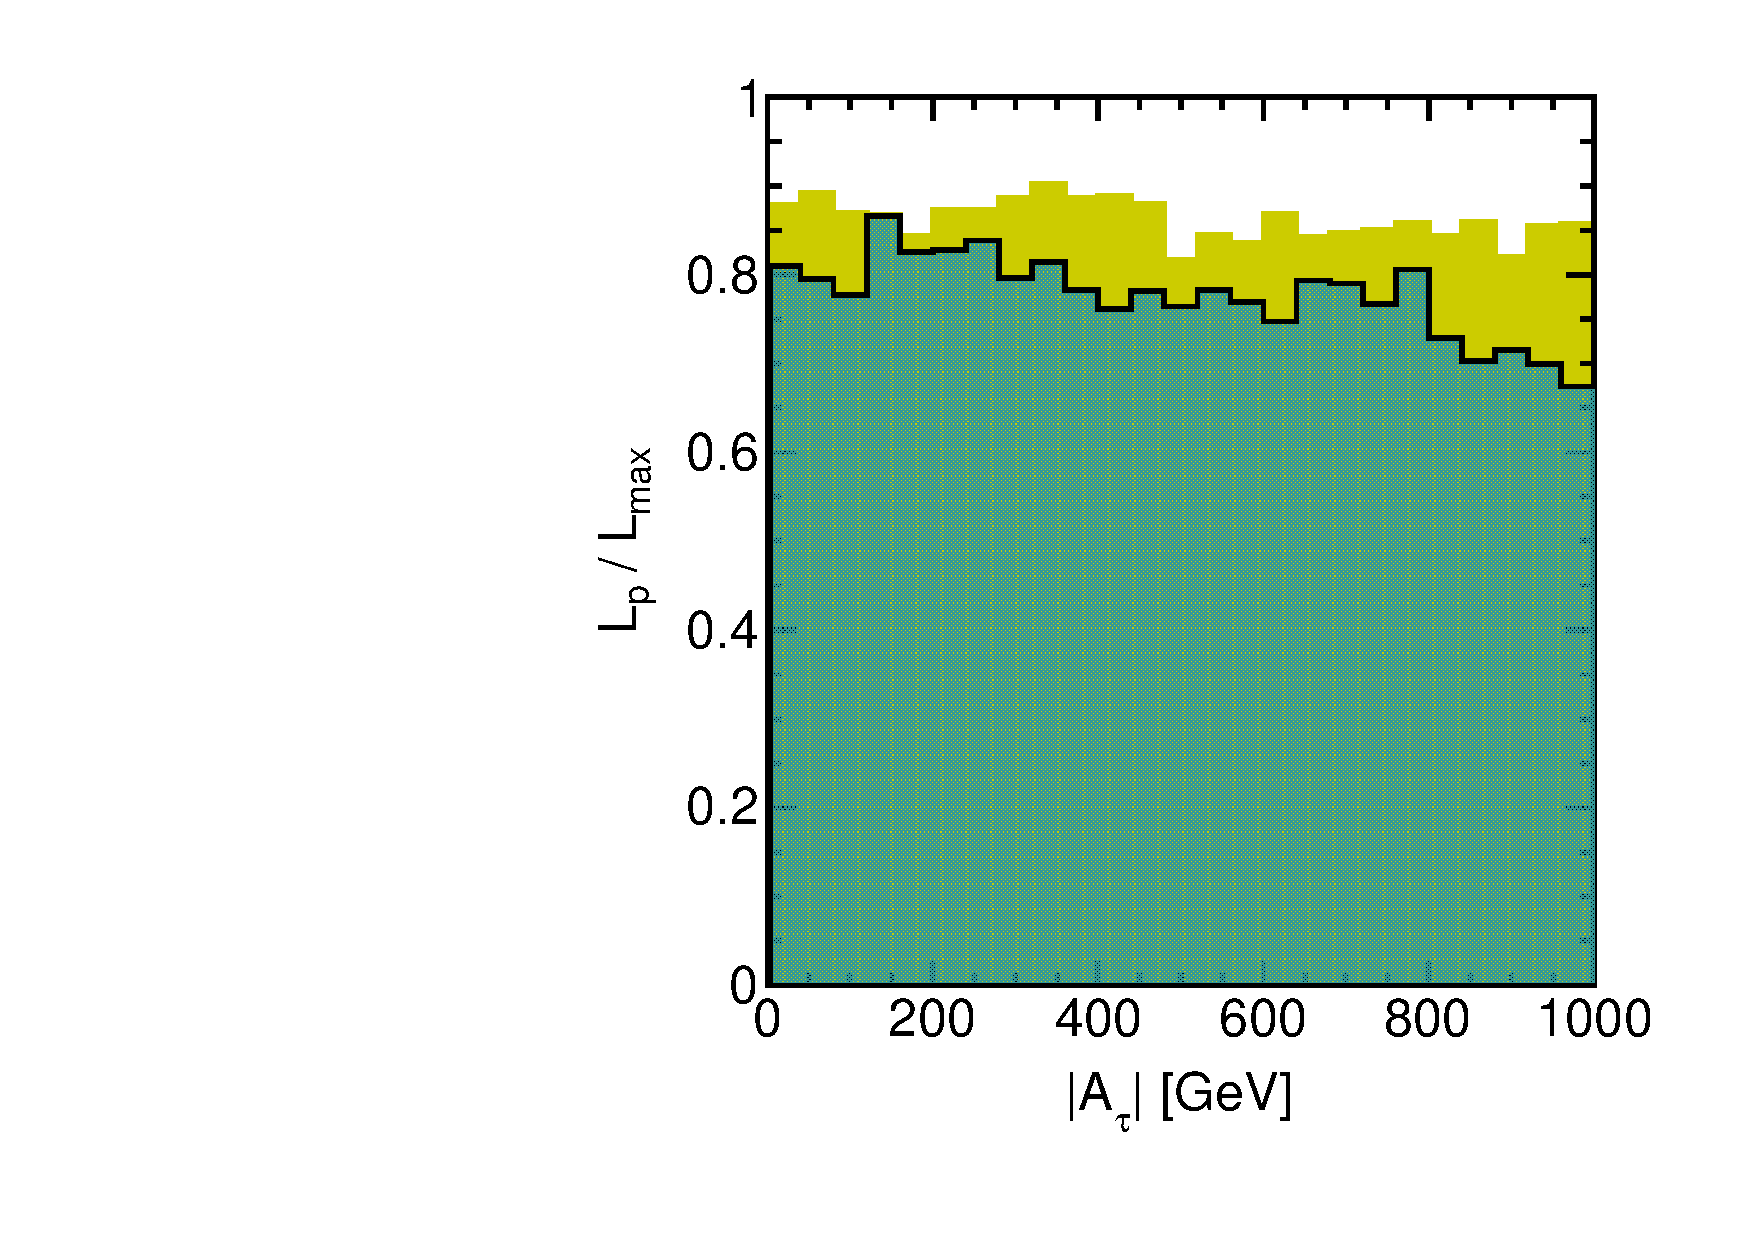
\includegraphics[height=5.5cm]{figs/fig_A_tau.pdf}
\caption{Ratios of profile likelihood $L_p$ to maximum likelihood $L_{max}$ shown for trilinear couplings at SUSY scale.  The colored and shaded histograms show the distributions before and after the inclusion of the CMS results.}
\label{fig:LRwcms_A}
\end{center}
\end{figure}

\begin{figure}[htbp]
\begin{center}
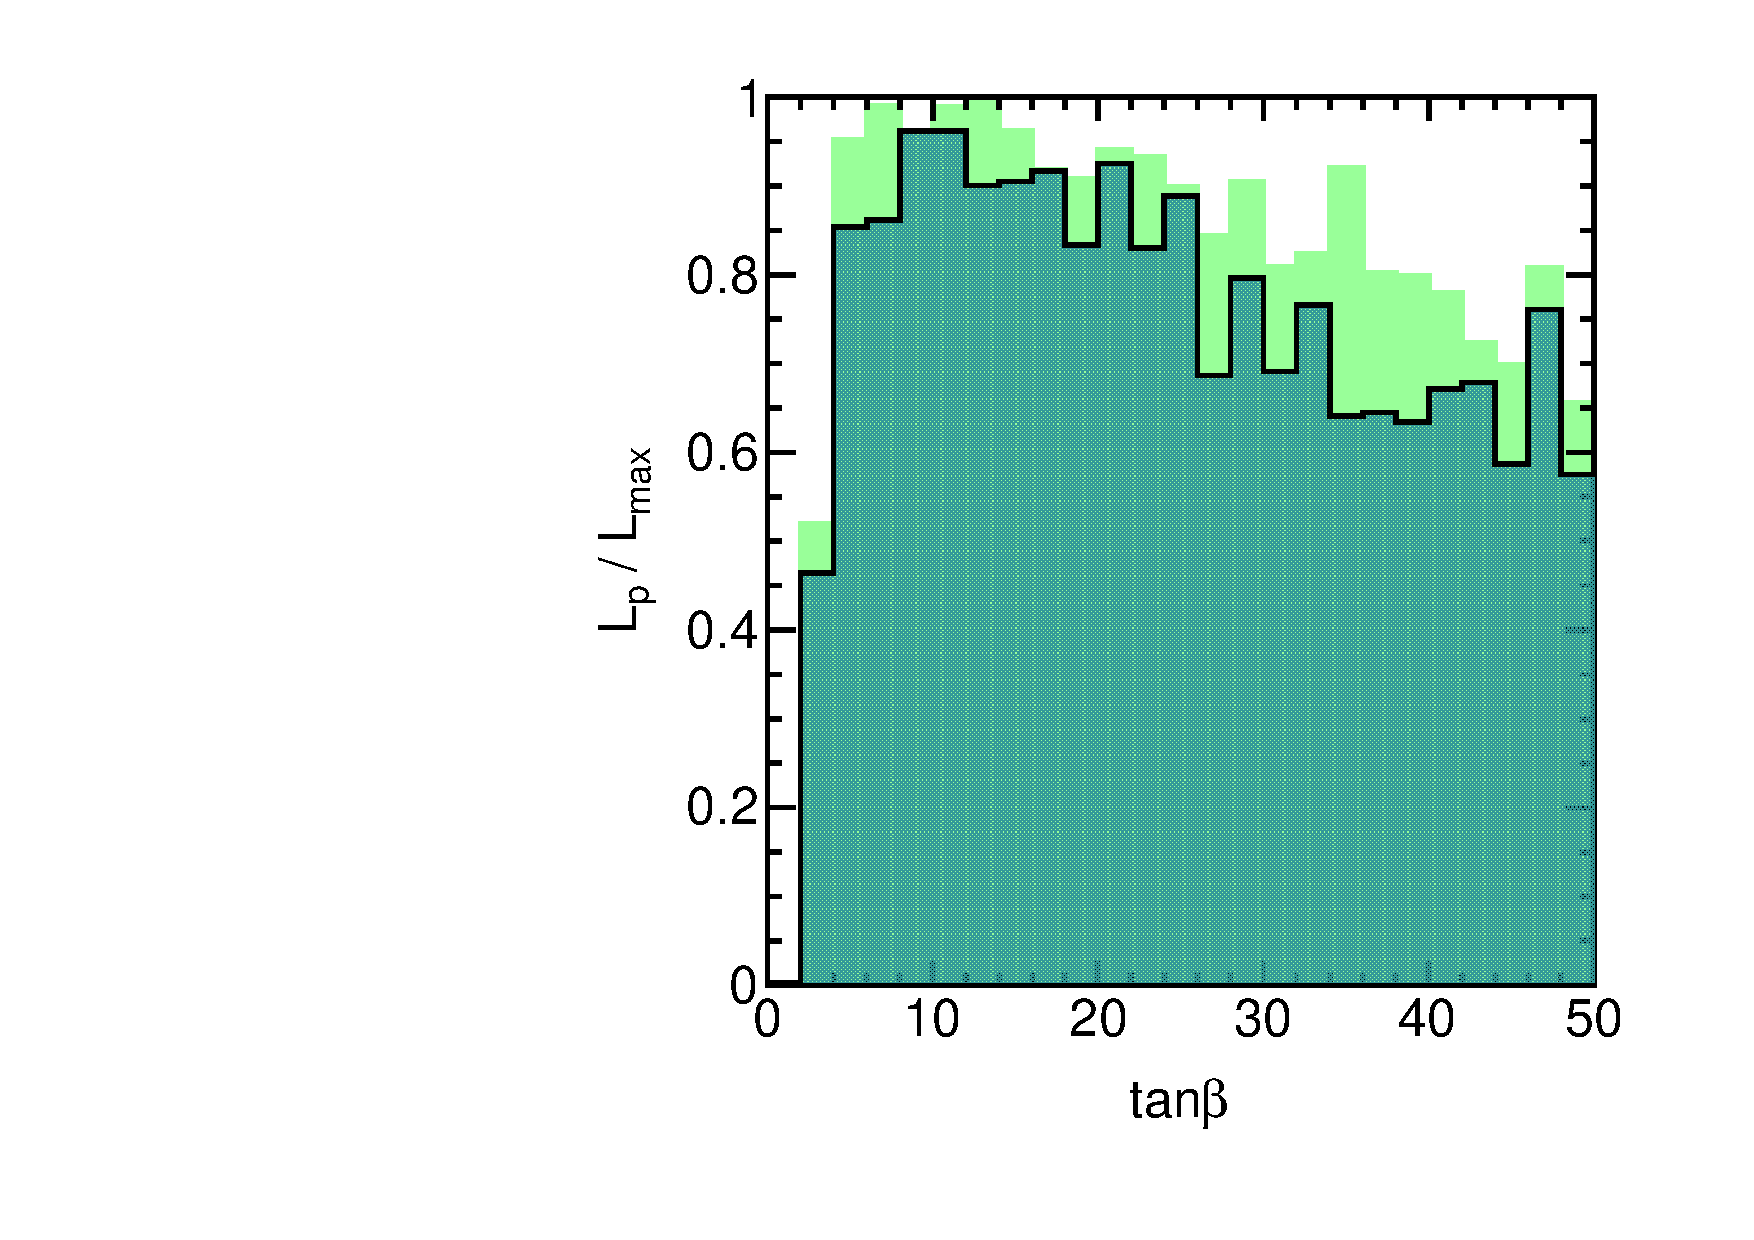
\includegraphics[height=5.5cm]{figs/fig_tanbeta.pdf} 
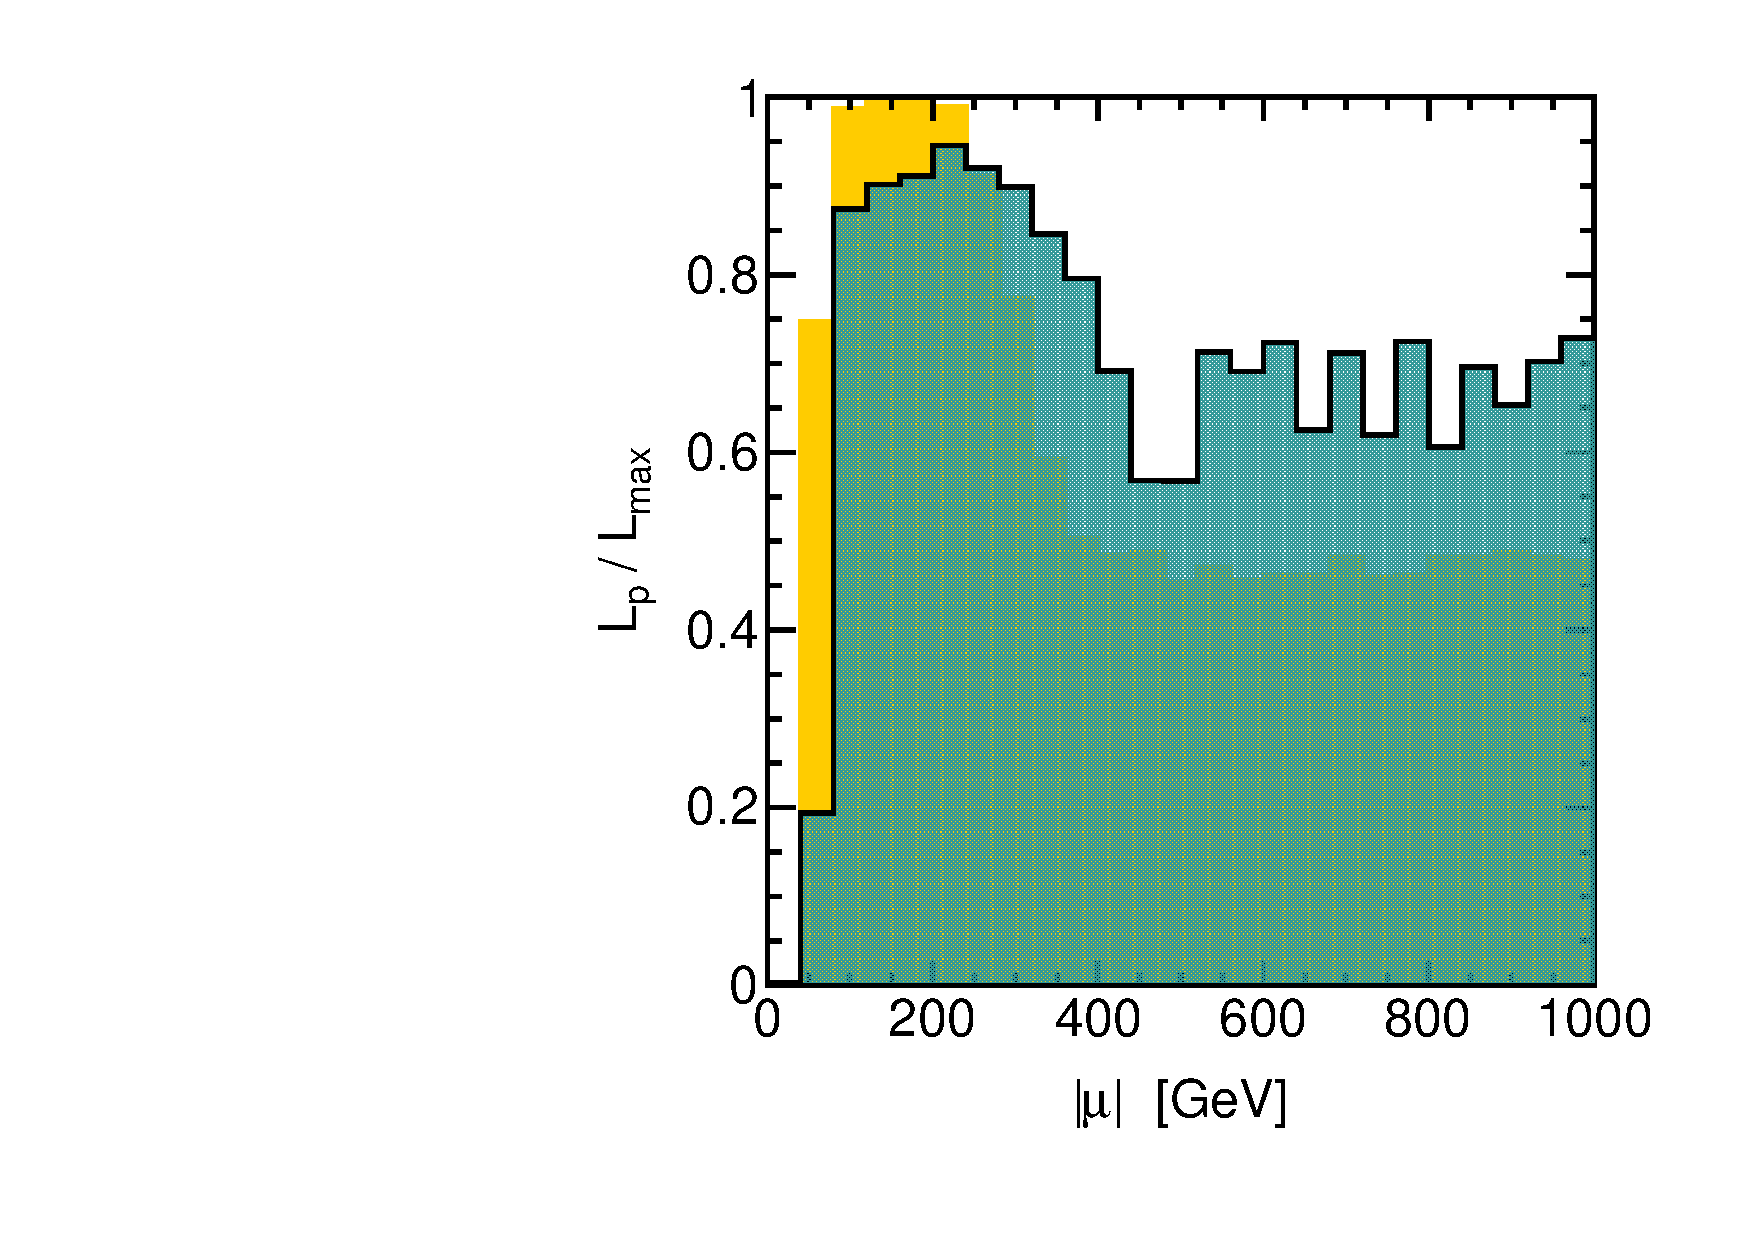
\includegraphics[height=5.5cm]{figs/fig_mu.pdf} 
\caption{Ratios of profile likelihood $L_p$ to maximum likelihood $L_{max}$ shown for $\tan\beta$ and $\mu$ parameter at SUSY scale.  The colored and shaded histograms show the distributions before and after the inclusion of the CMS results.}
\label{fig:LRwcms_tbmu}
\end{center}
\end{figure}



\begin{figure}[htbp]
\begin{center}
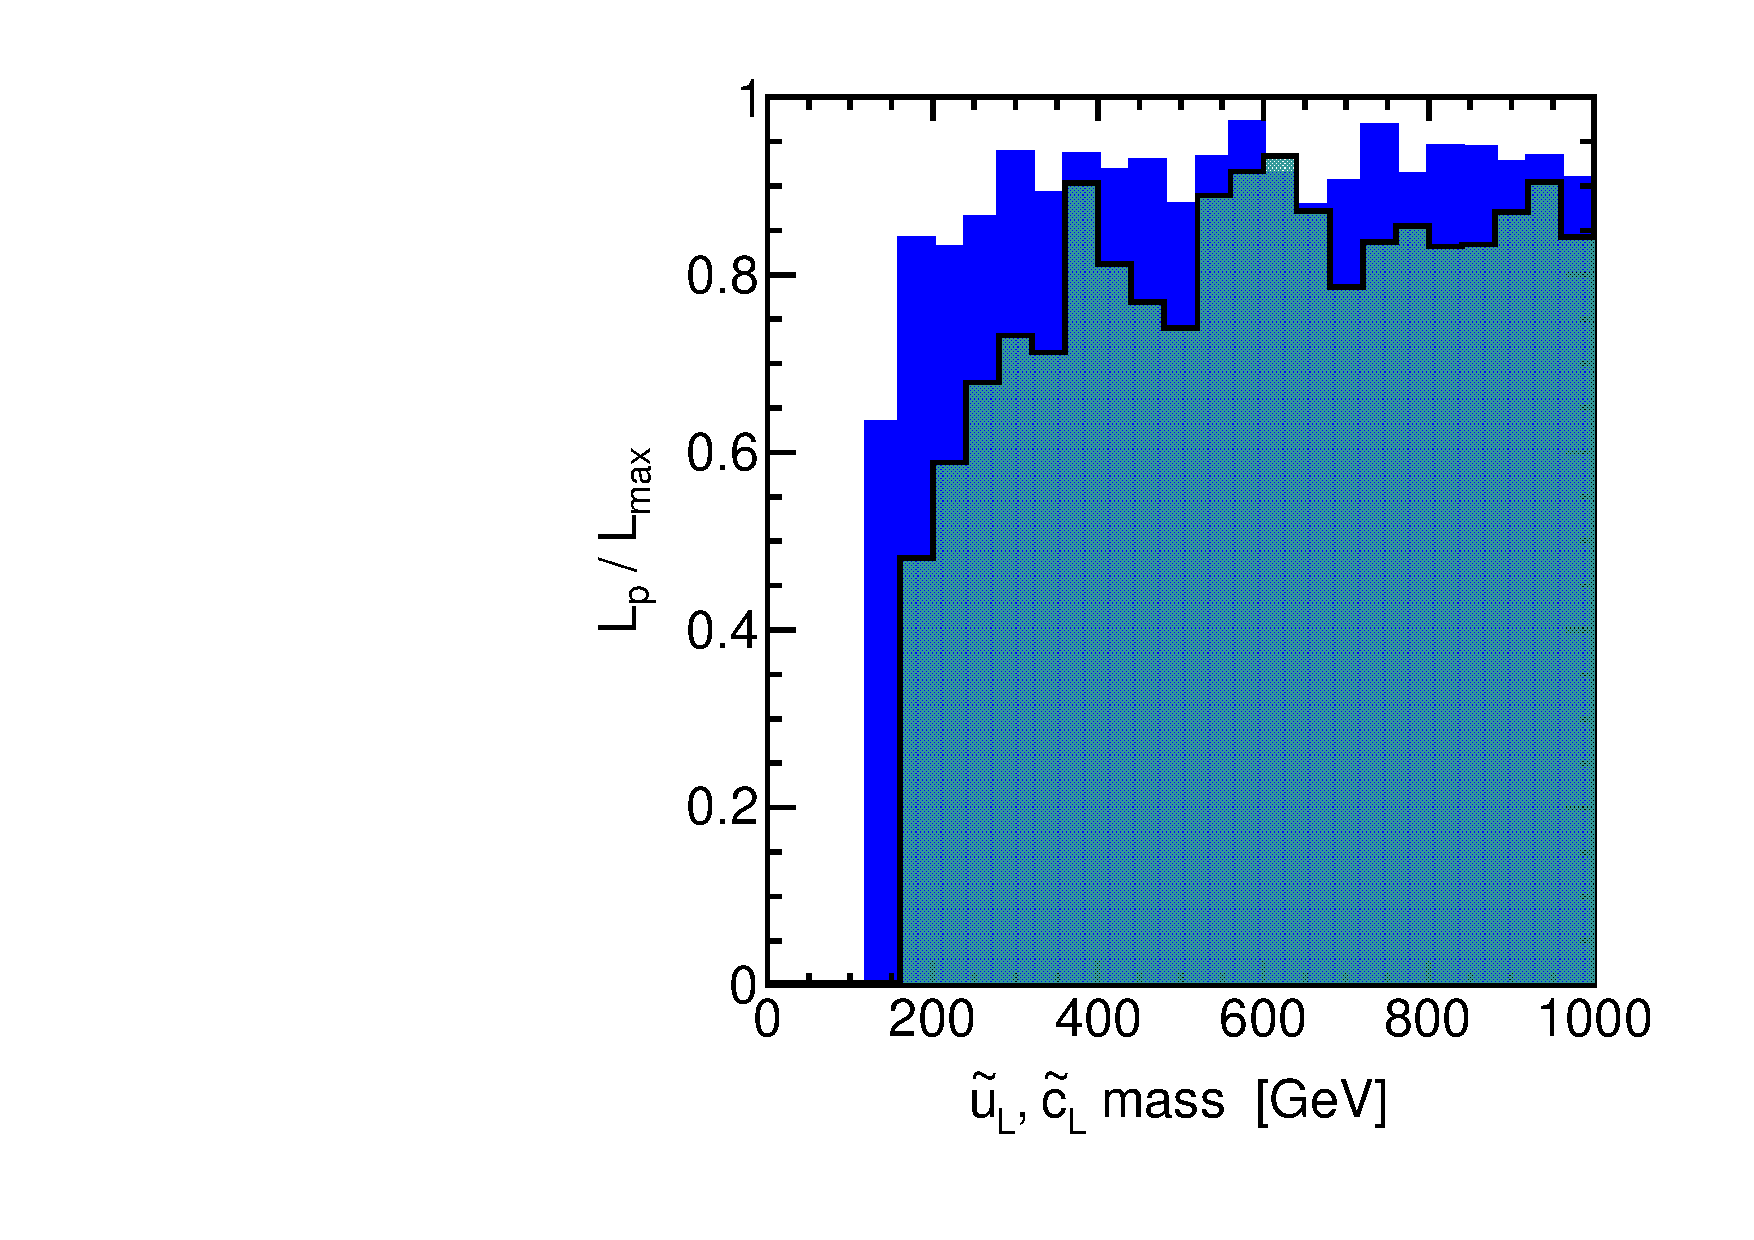
\includegraphics[height=5.5cm]{figs/fig_u_L.pdf} 
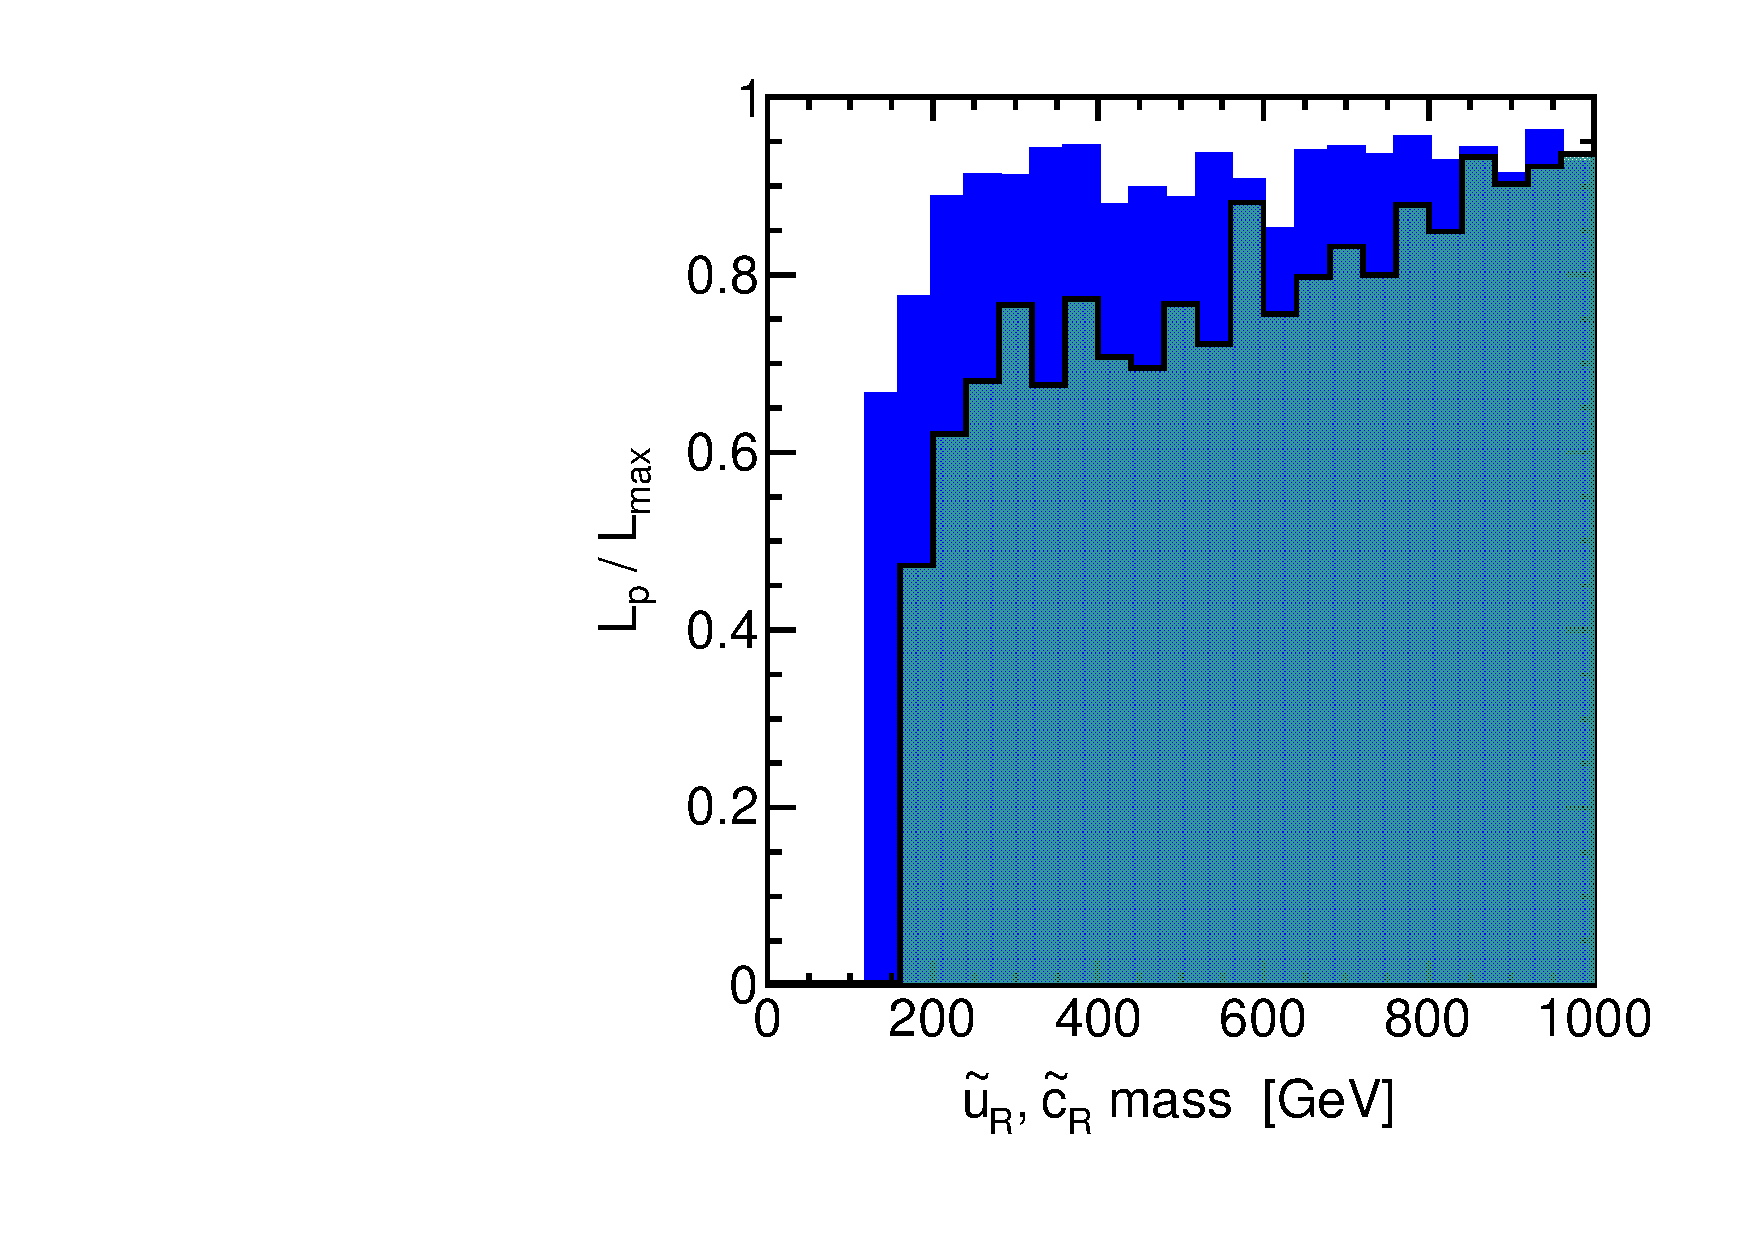
\includegraphics[height=5.5cm]{figs/fig_u_R.pdf} \\
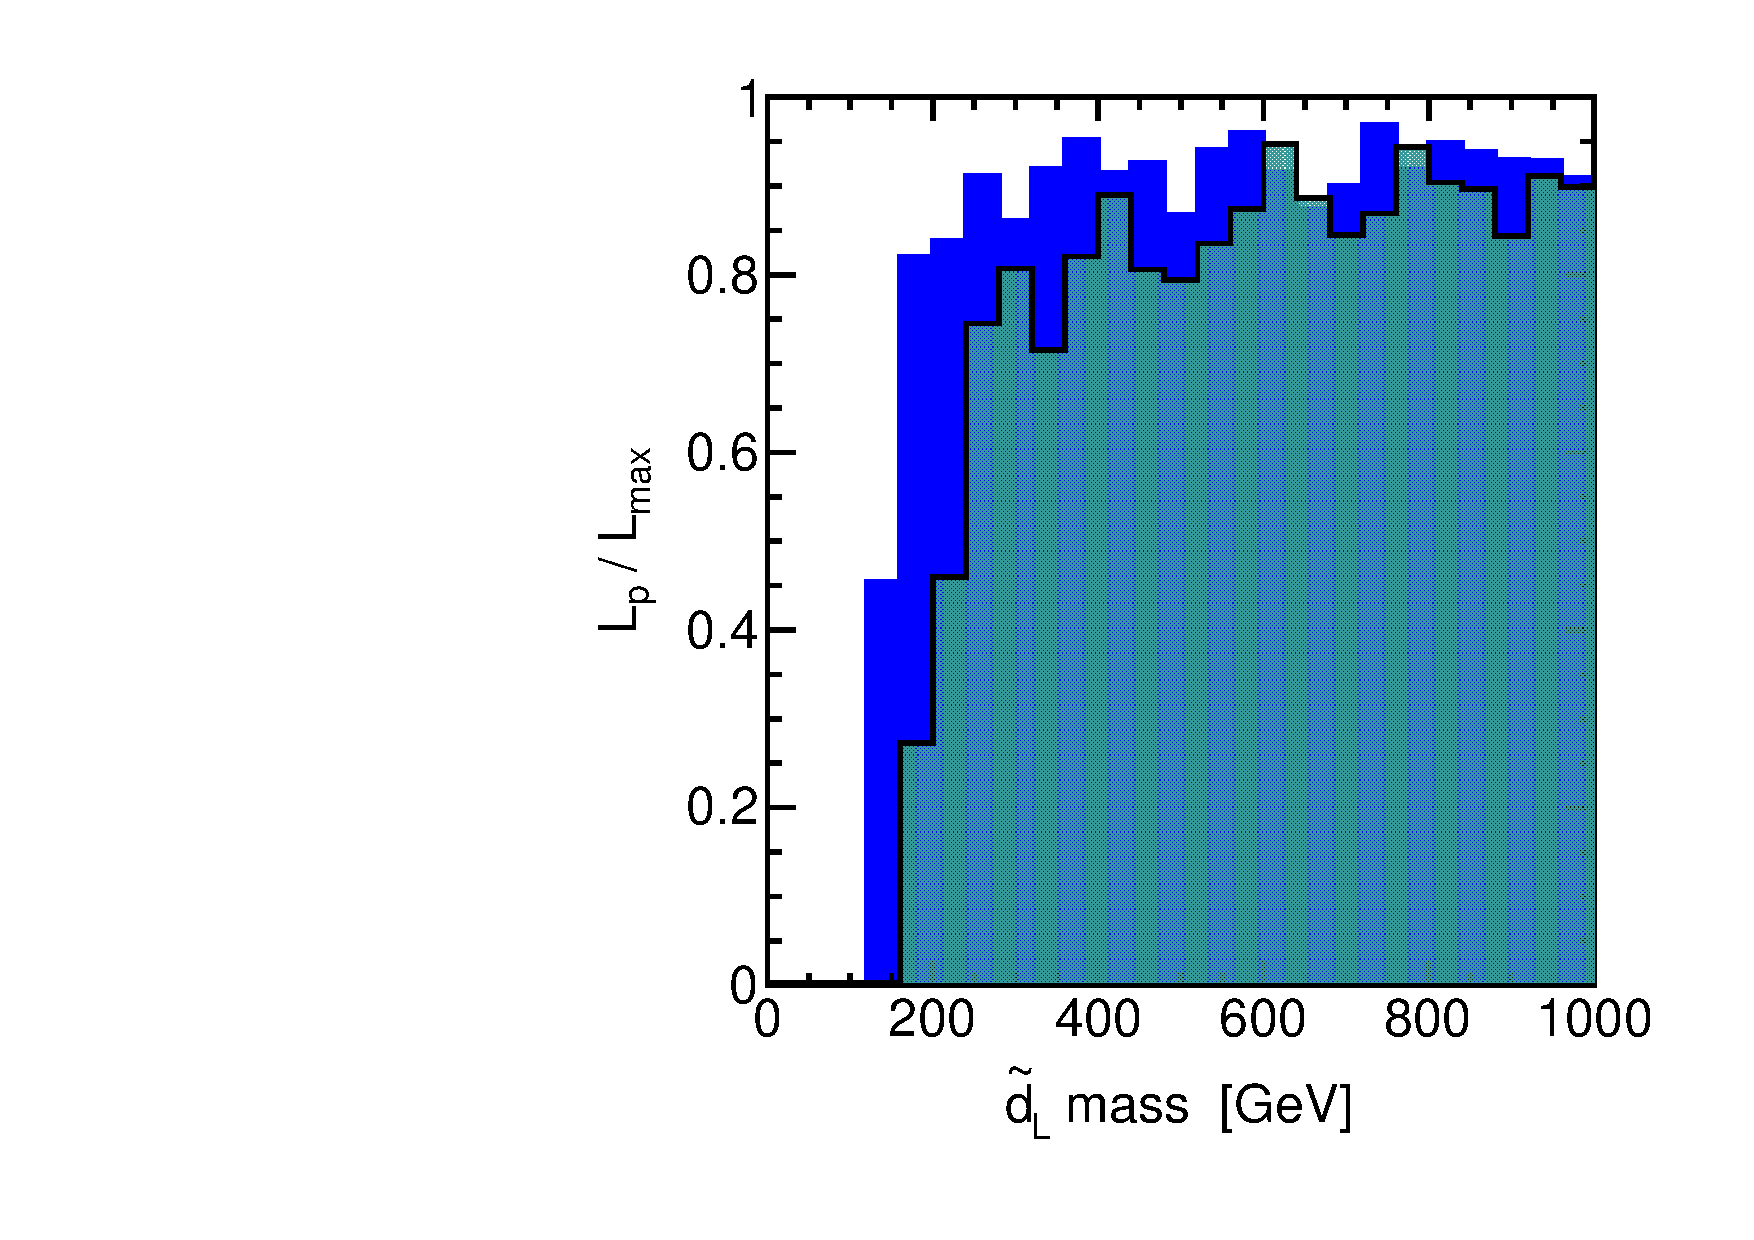
\includegraphics[height=5.5cm]{figs/fig_d_L.pdf} 
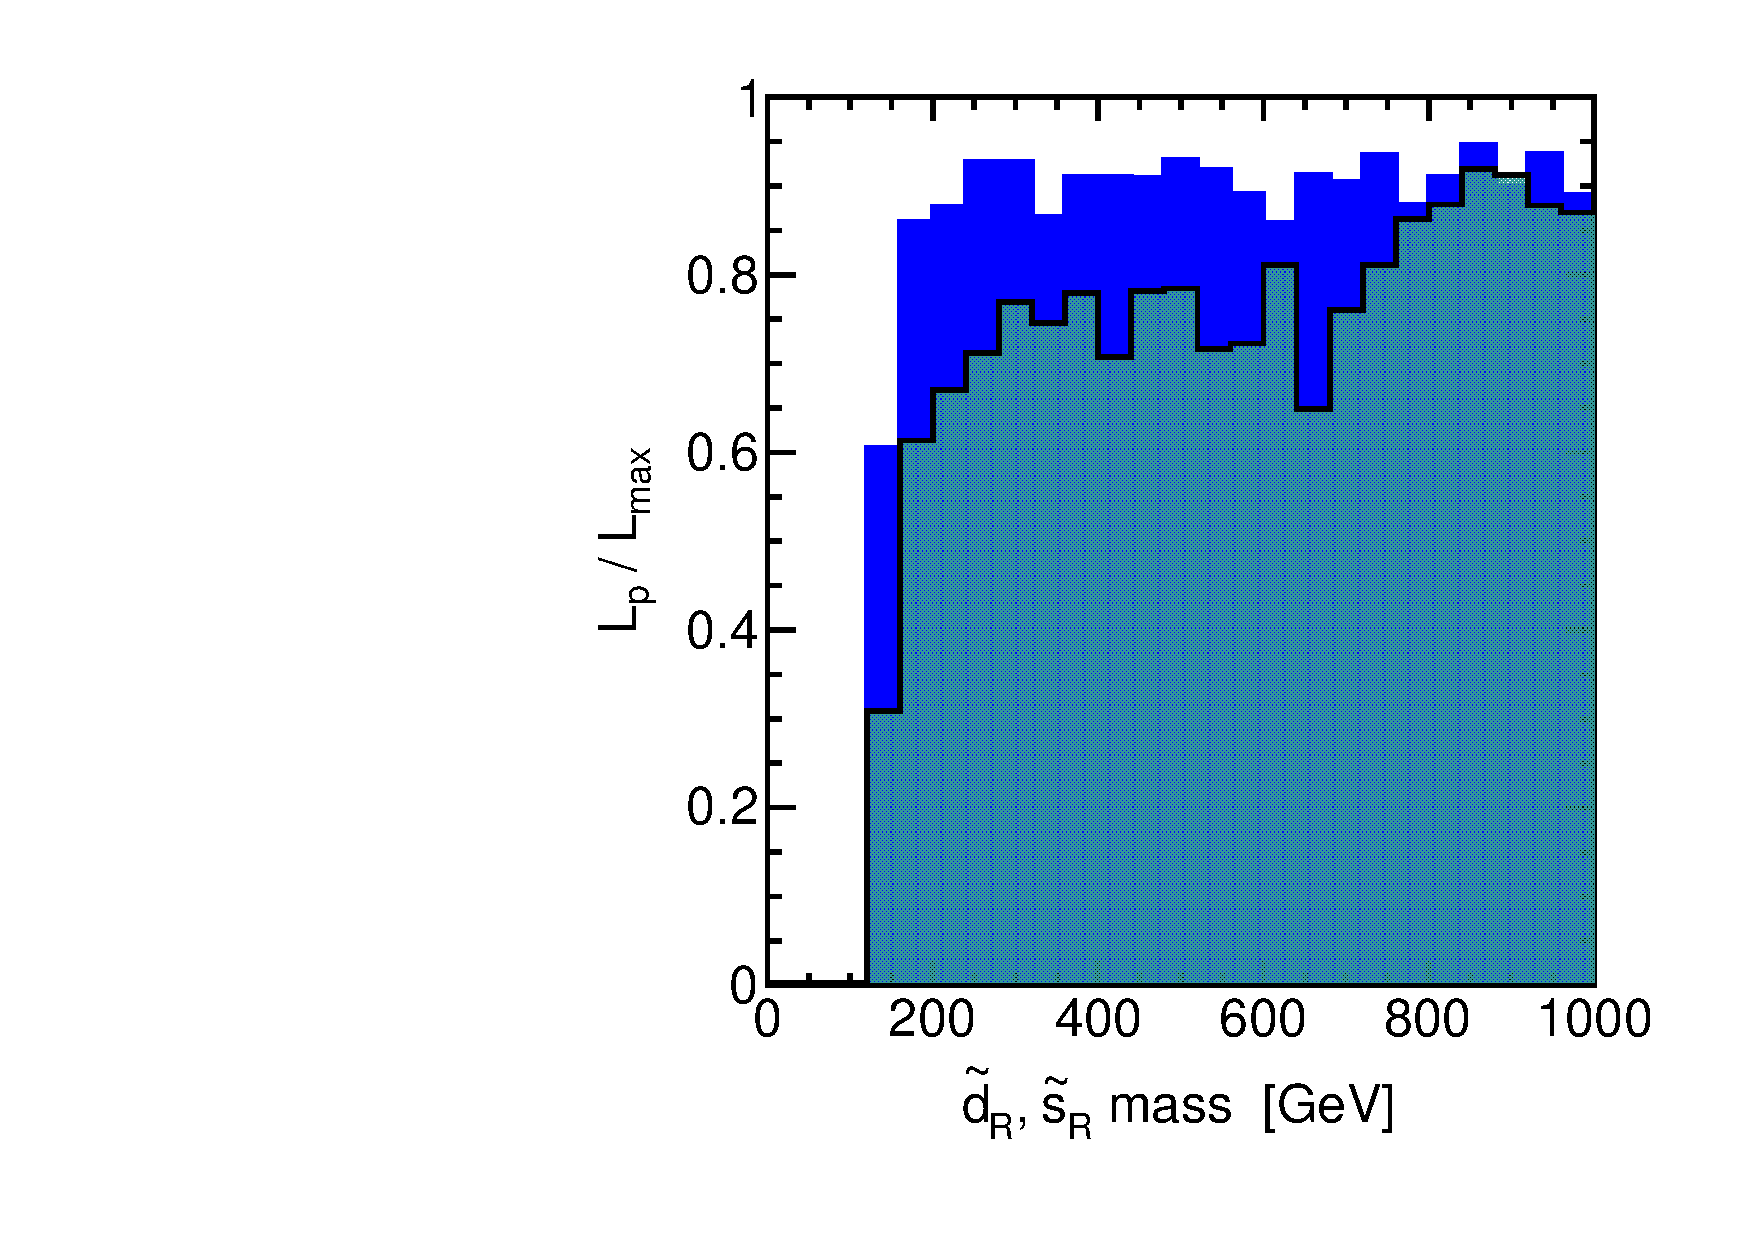
\includegraphics[height=5.5cm]{figs/fig_d_R.pdf} \\
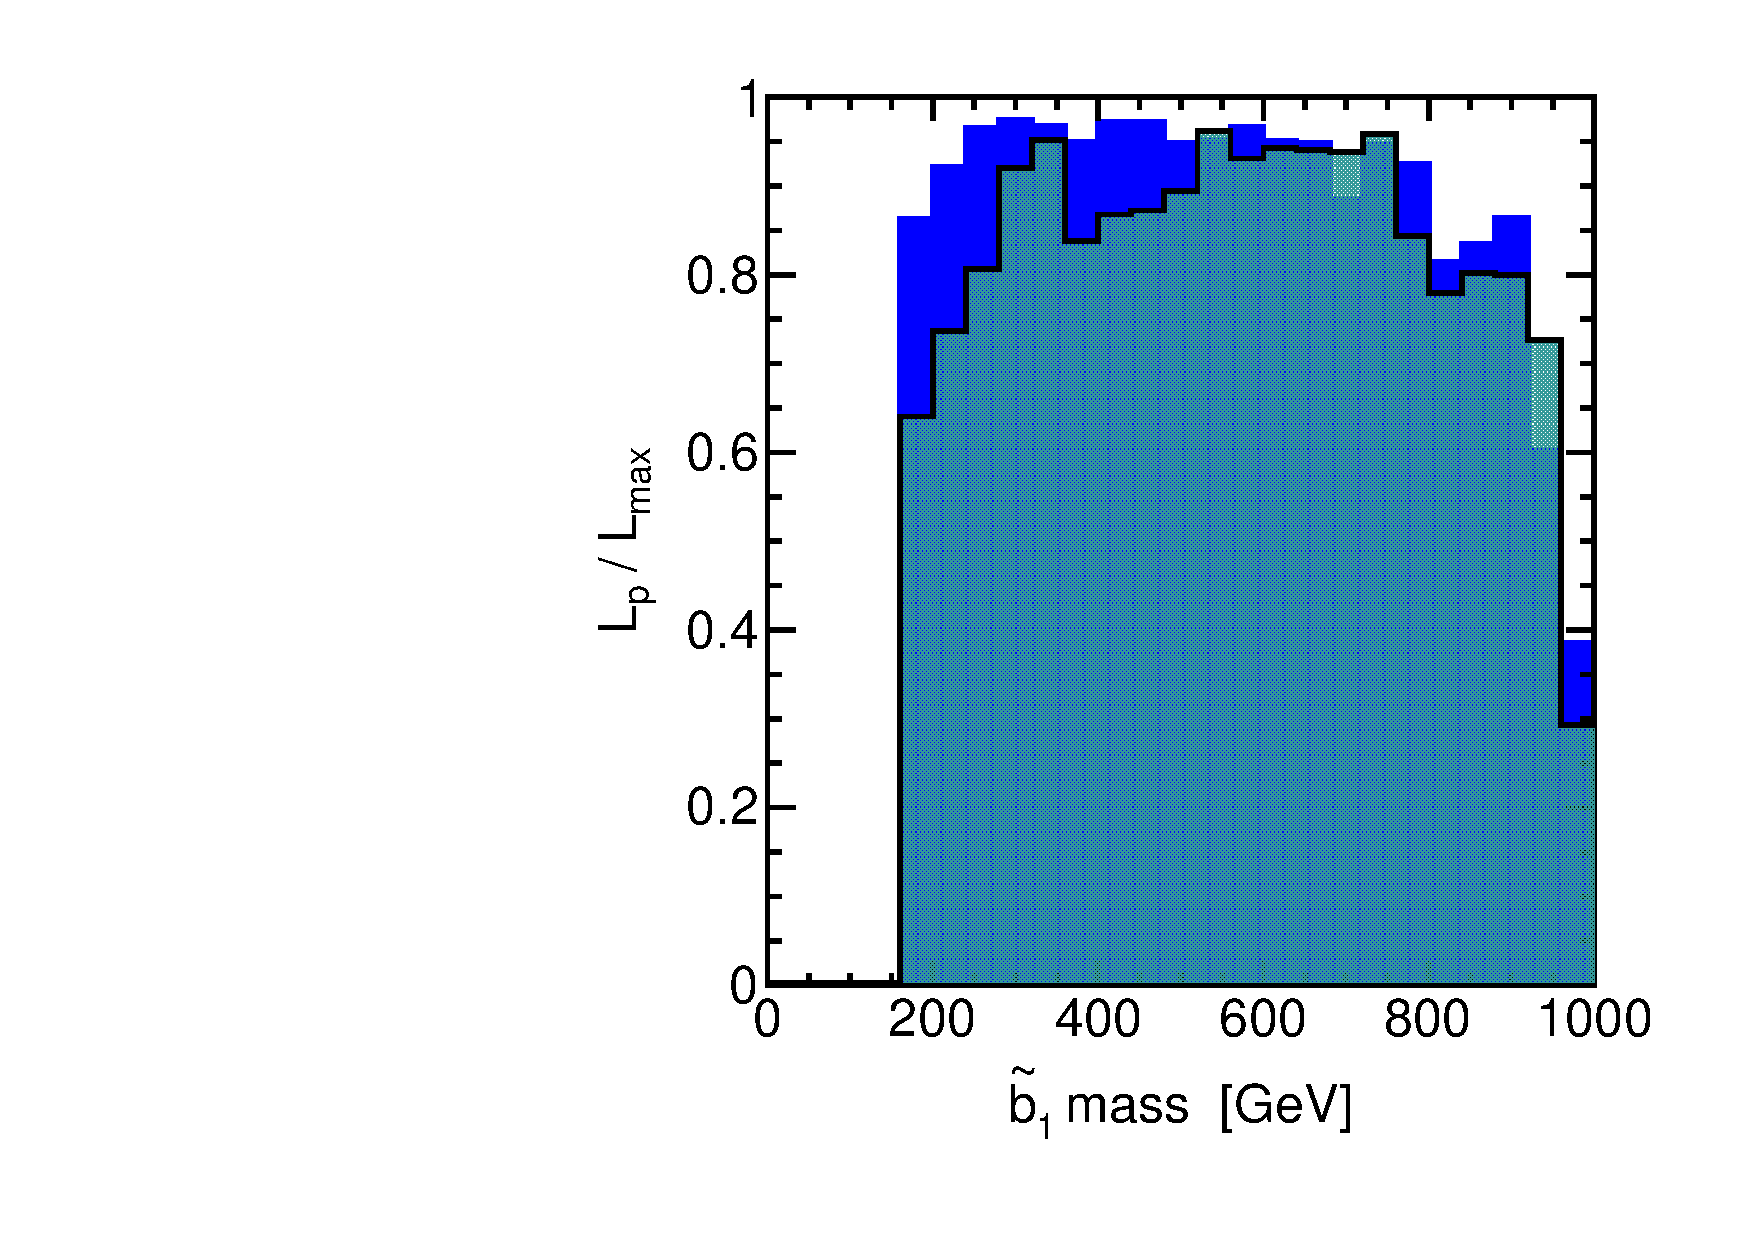
\includegraphics[height=5.5cm]{figs/fig_b_1.pdf} 
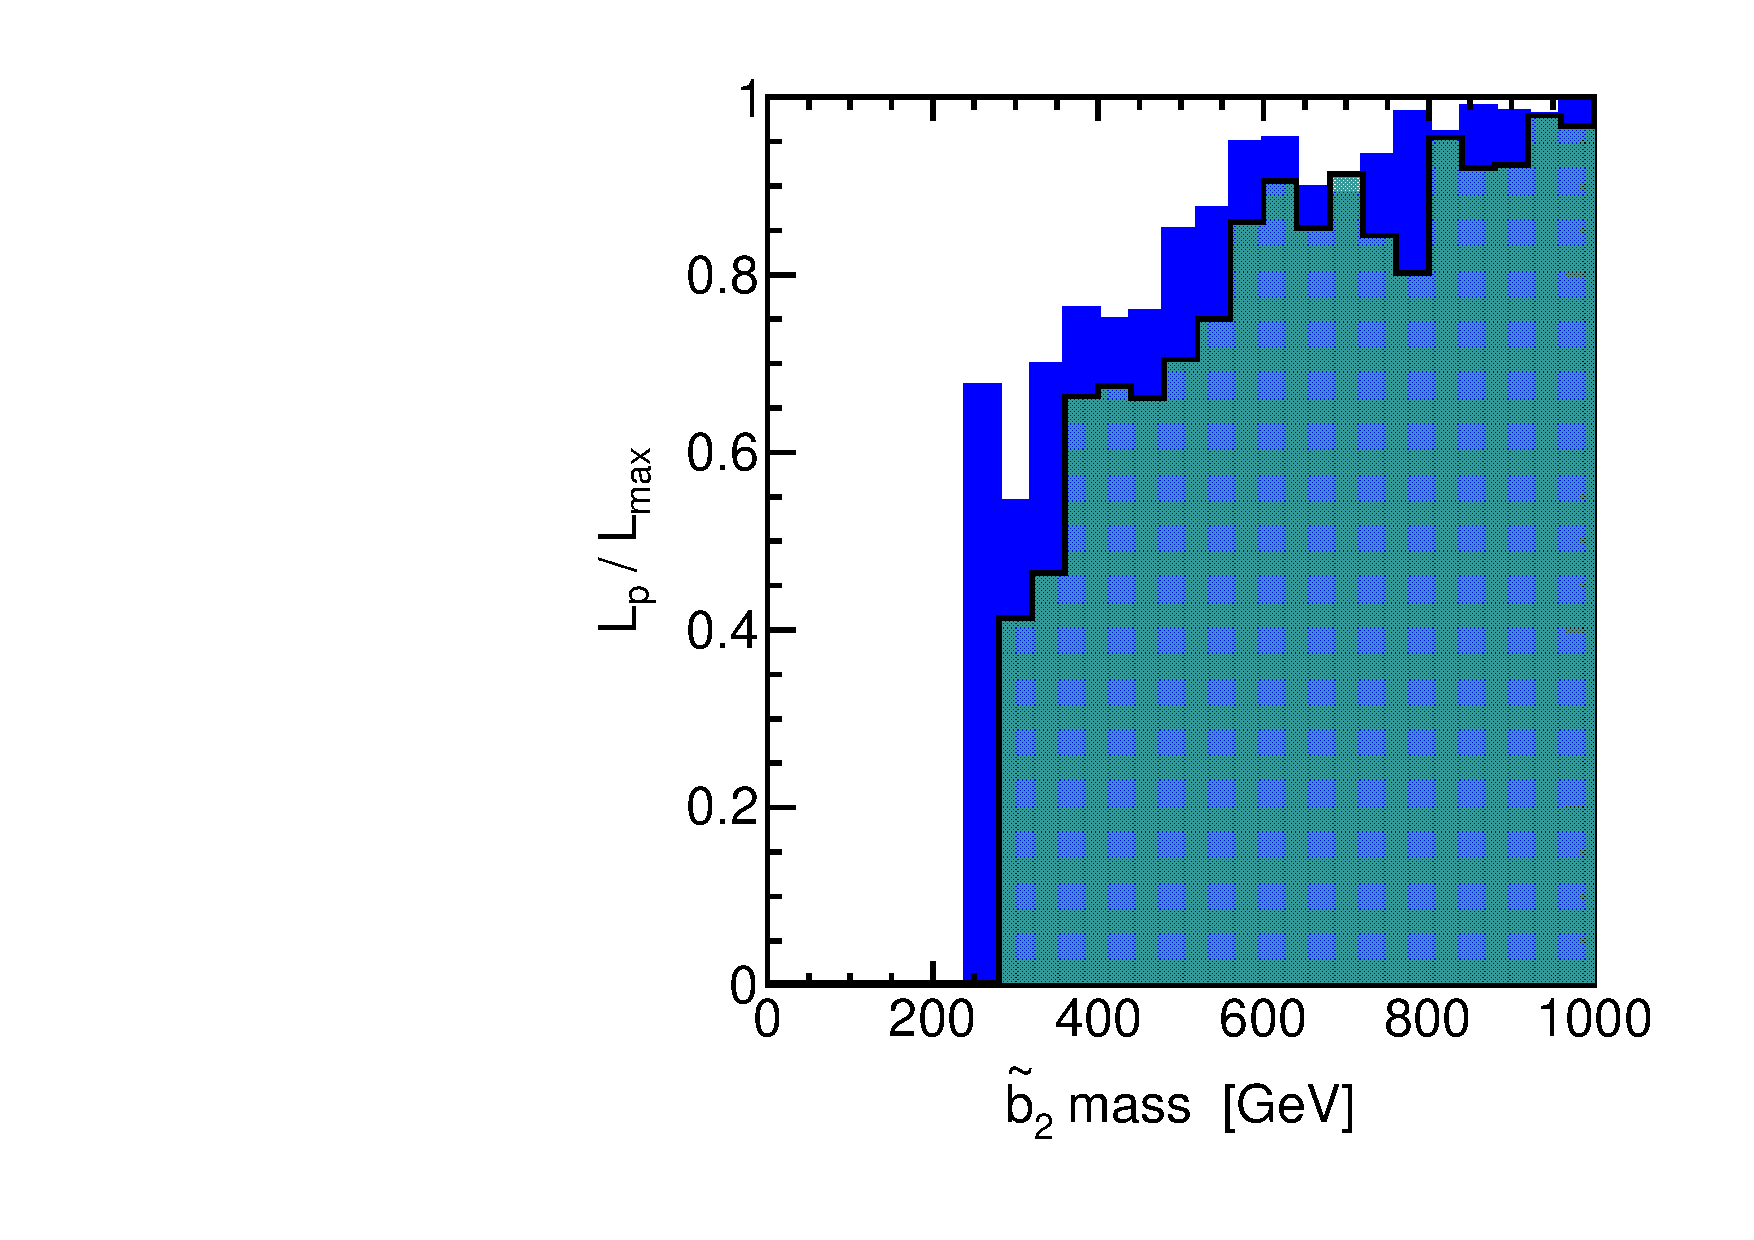
\includegraphics[height=5.5cm]{figs/fig_b_2.pdf} \\
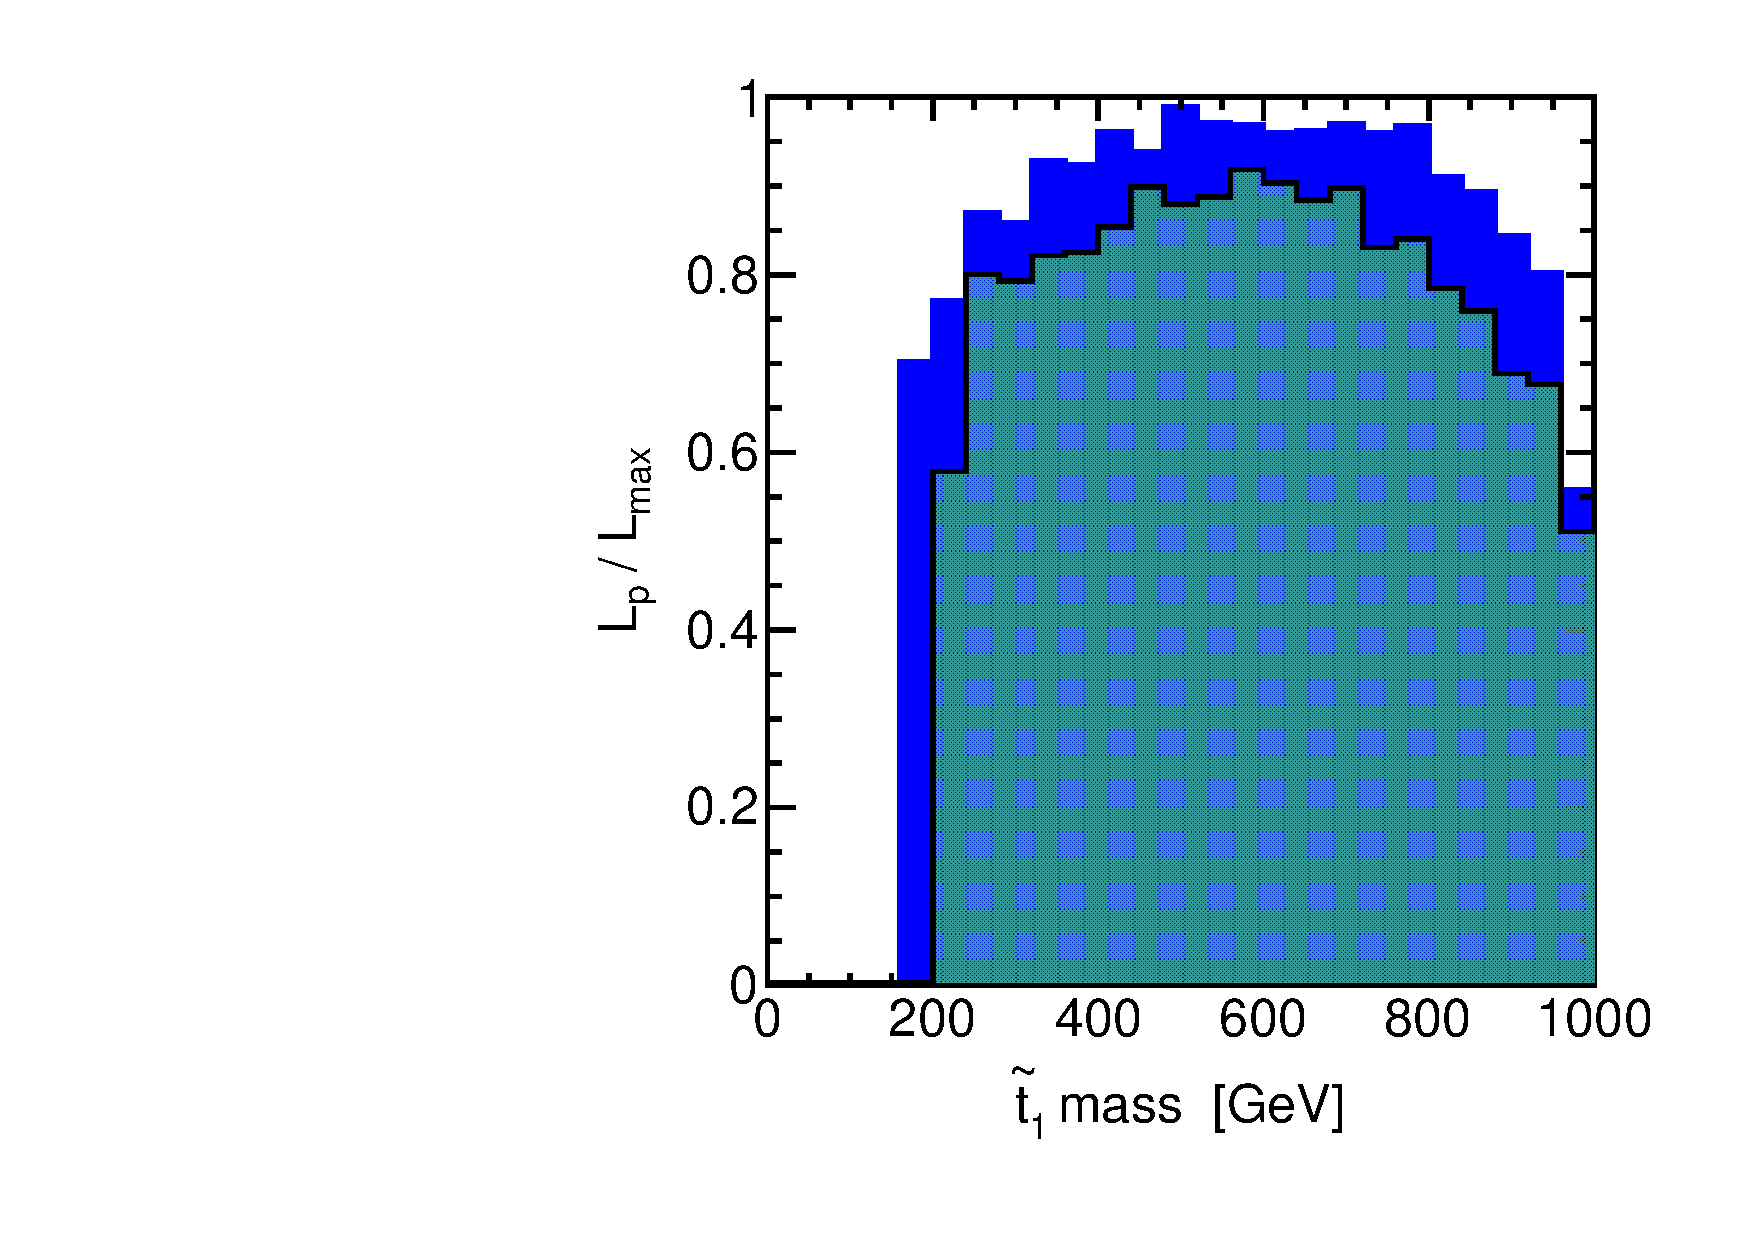
\includegraphics[height=5.5cm]{figs/fig_t_1.pdf} 
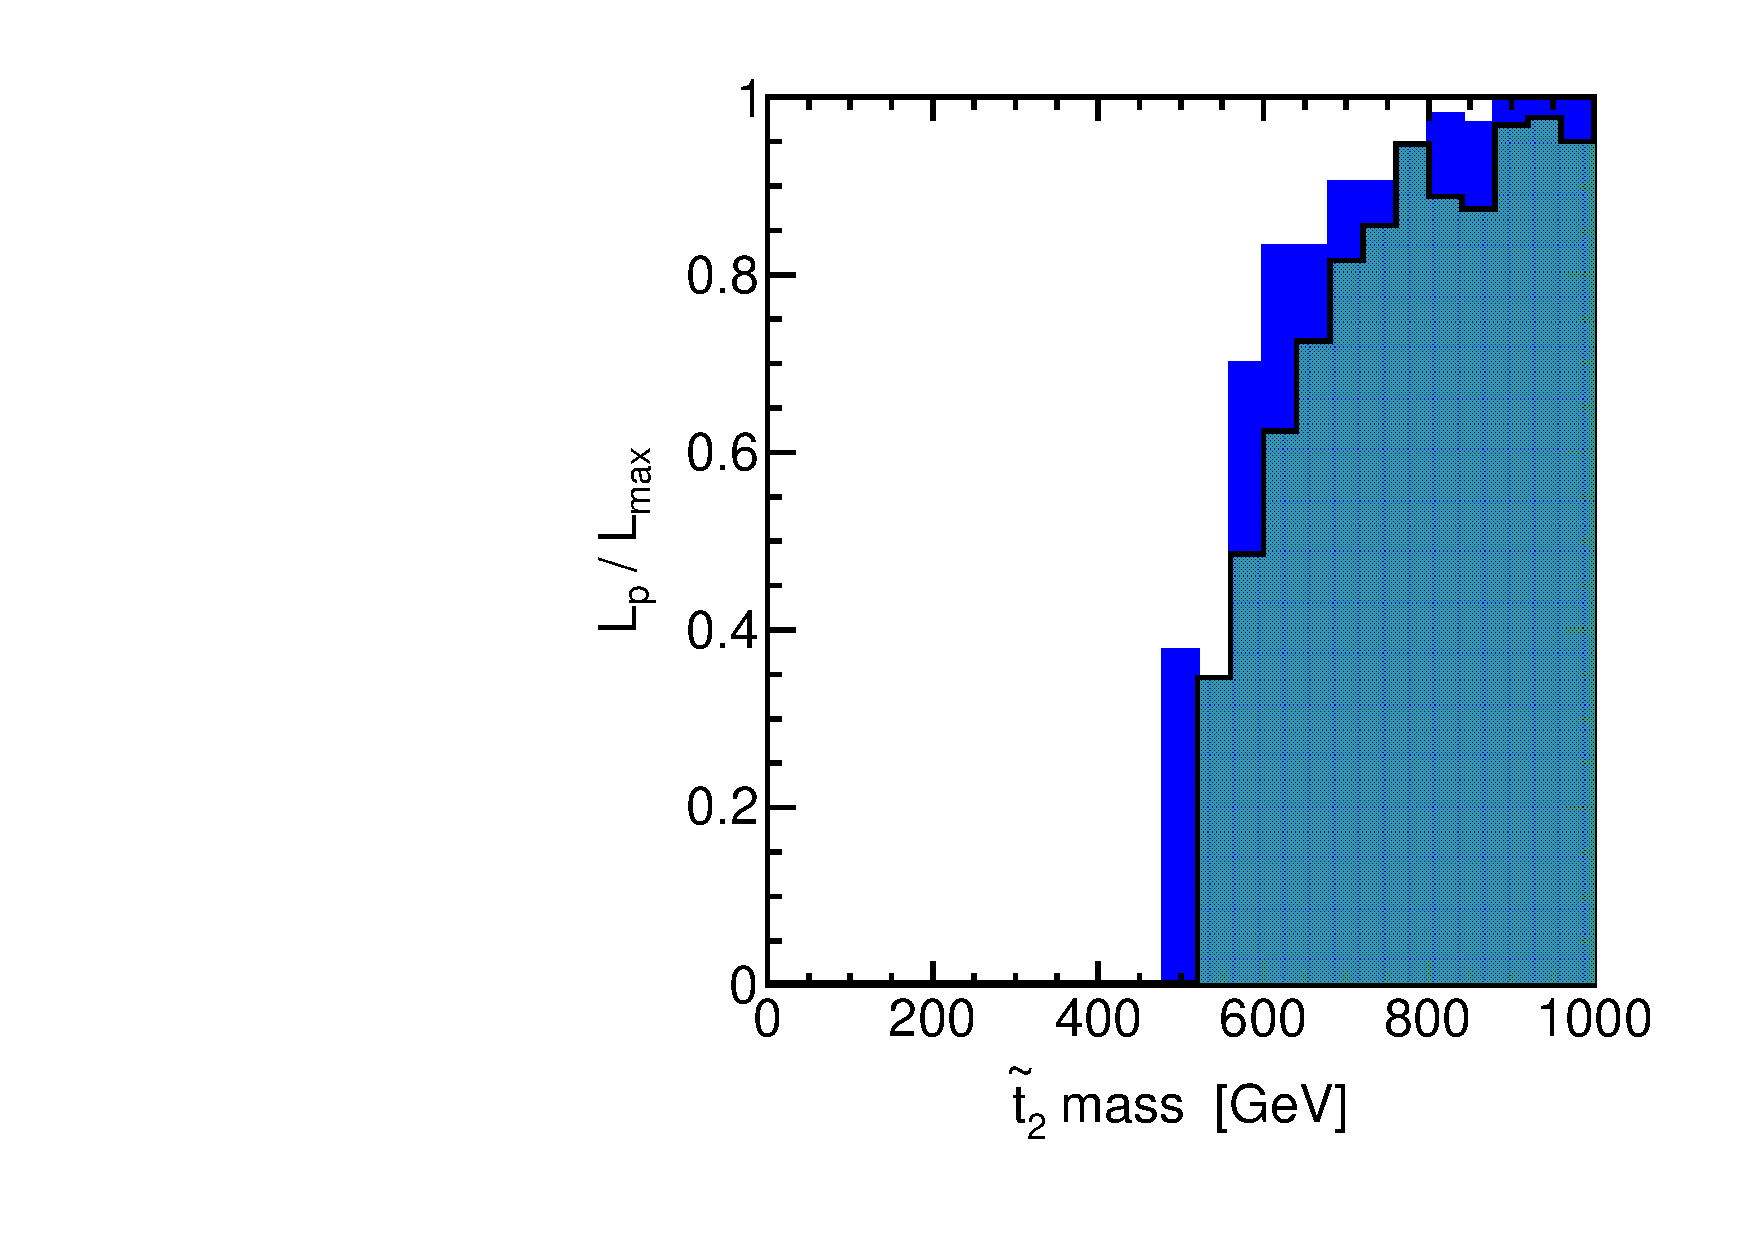
\includegraphics[height=5.5cm]{figs/fig_t_2.pdf} \\
\caption{Ratios of profile likelihood $L_p$ to maximum likelihood $L_{max}$ shown for squark masses.  The colored and shaded histograms show the distributions before and after the inclusion of the CMS results.}
\label{fig:LRwcms_sq}
\end{center}
\end{figure}


\begin{figure}[htbp]
\begin{center}
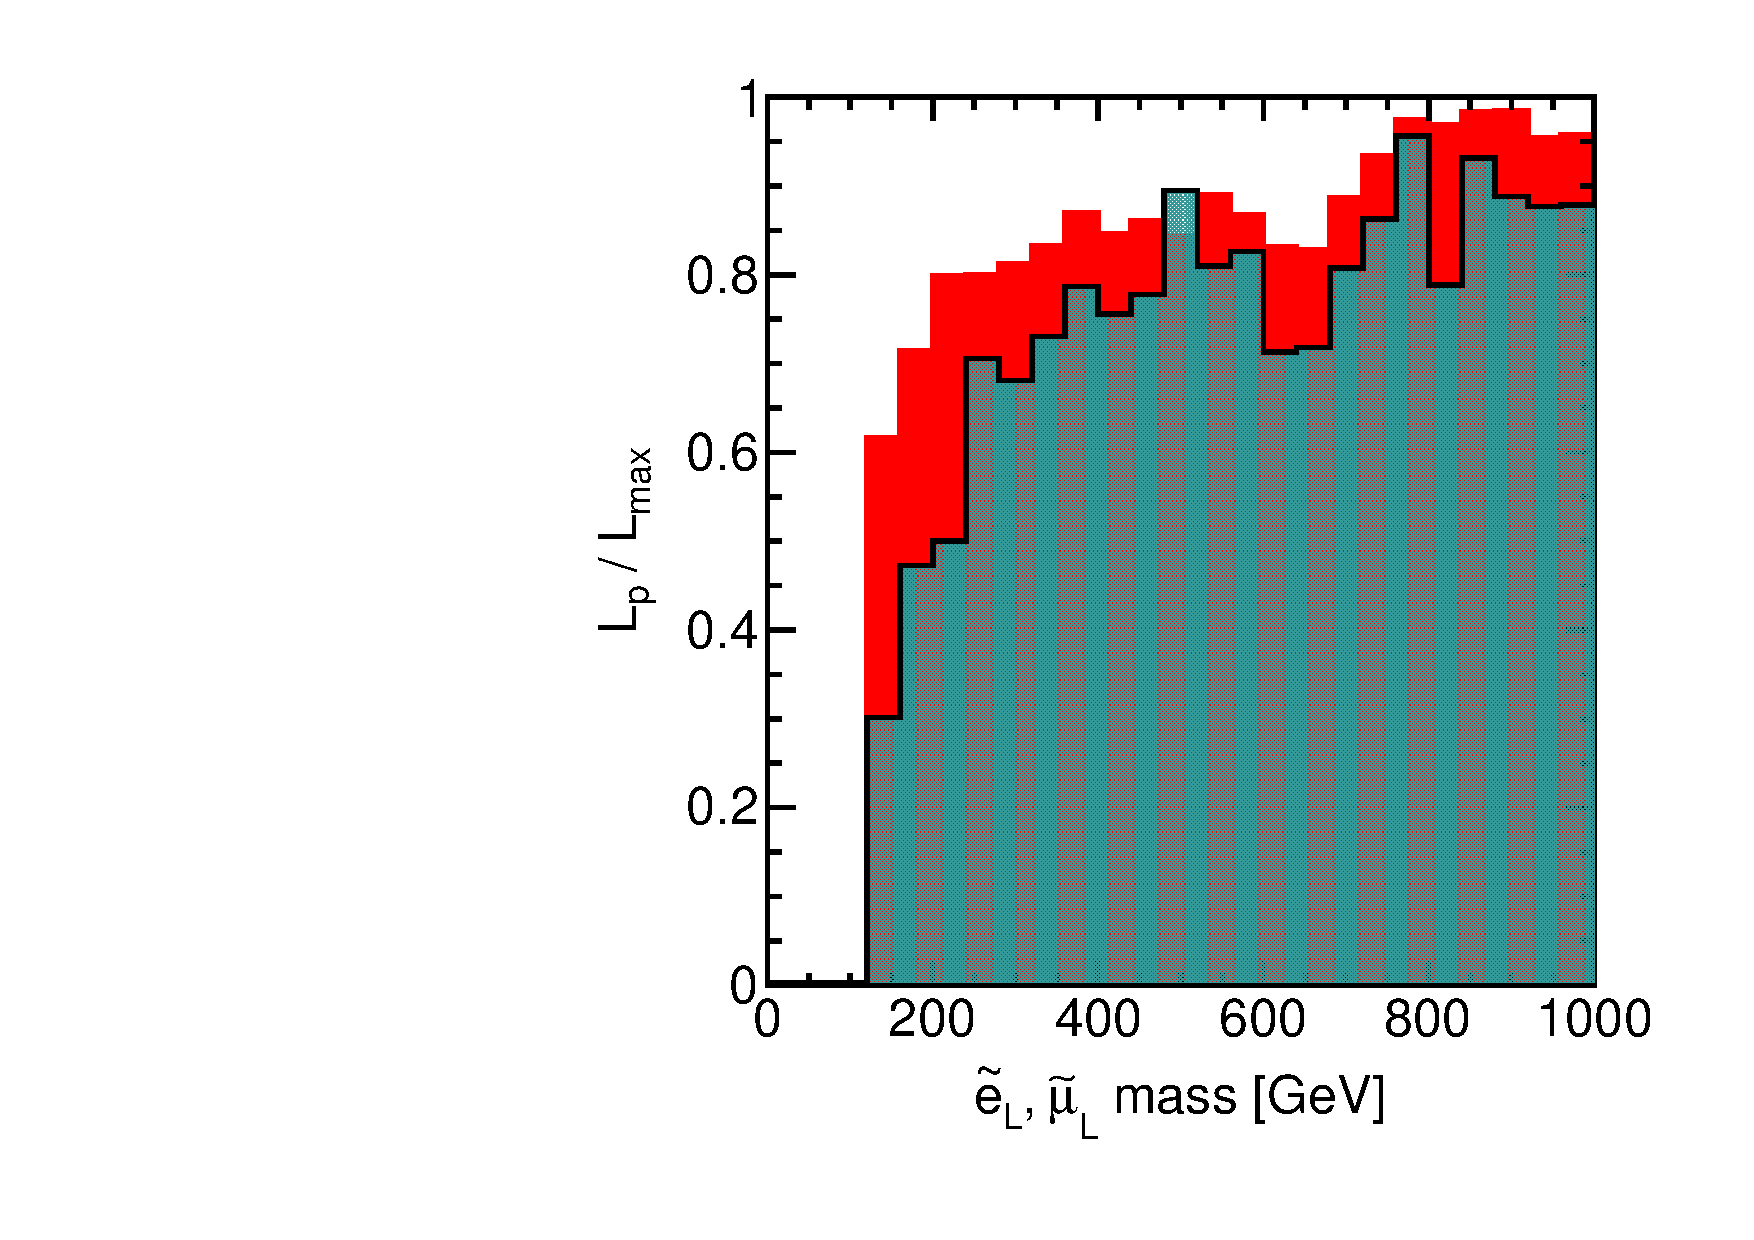
\includegraphics[height=5.5cm]{figs/fig_e_L.pdf} 
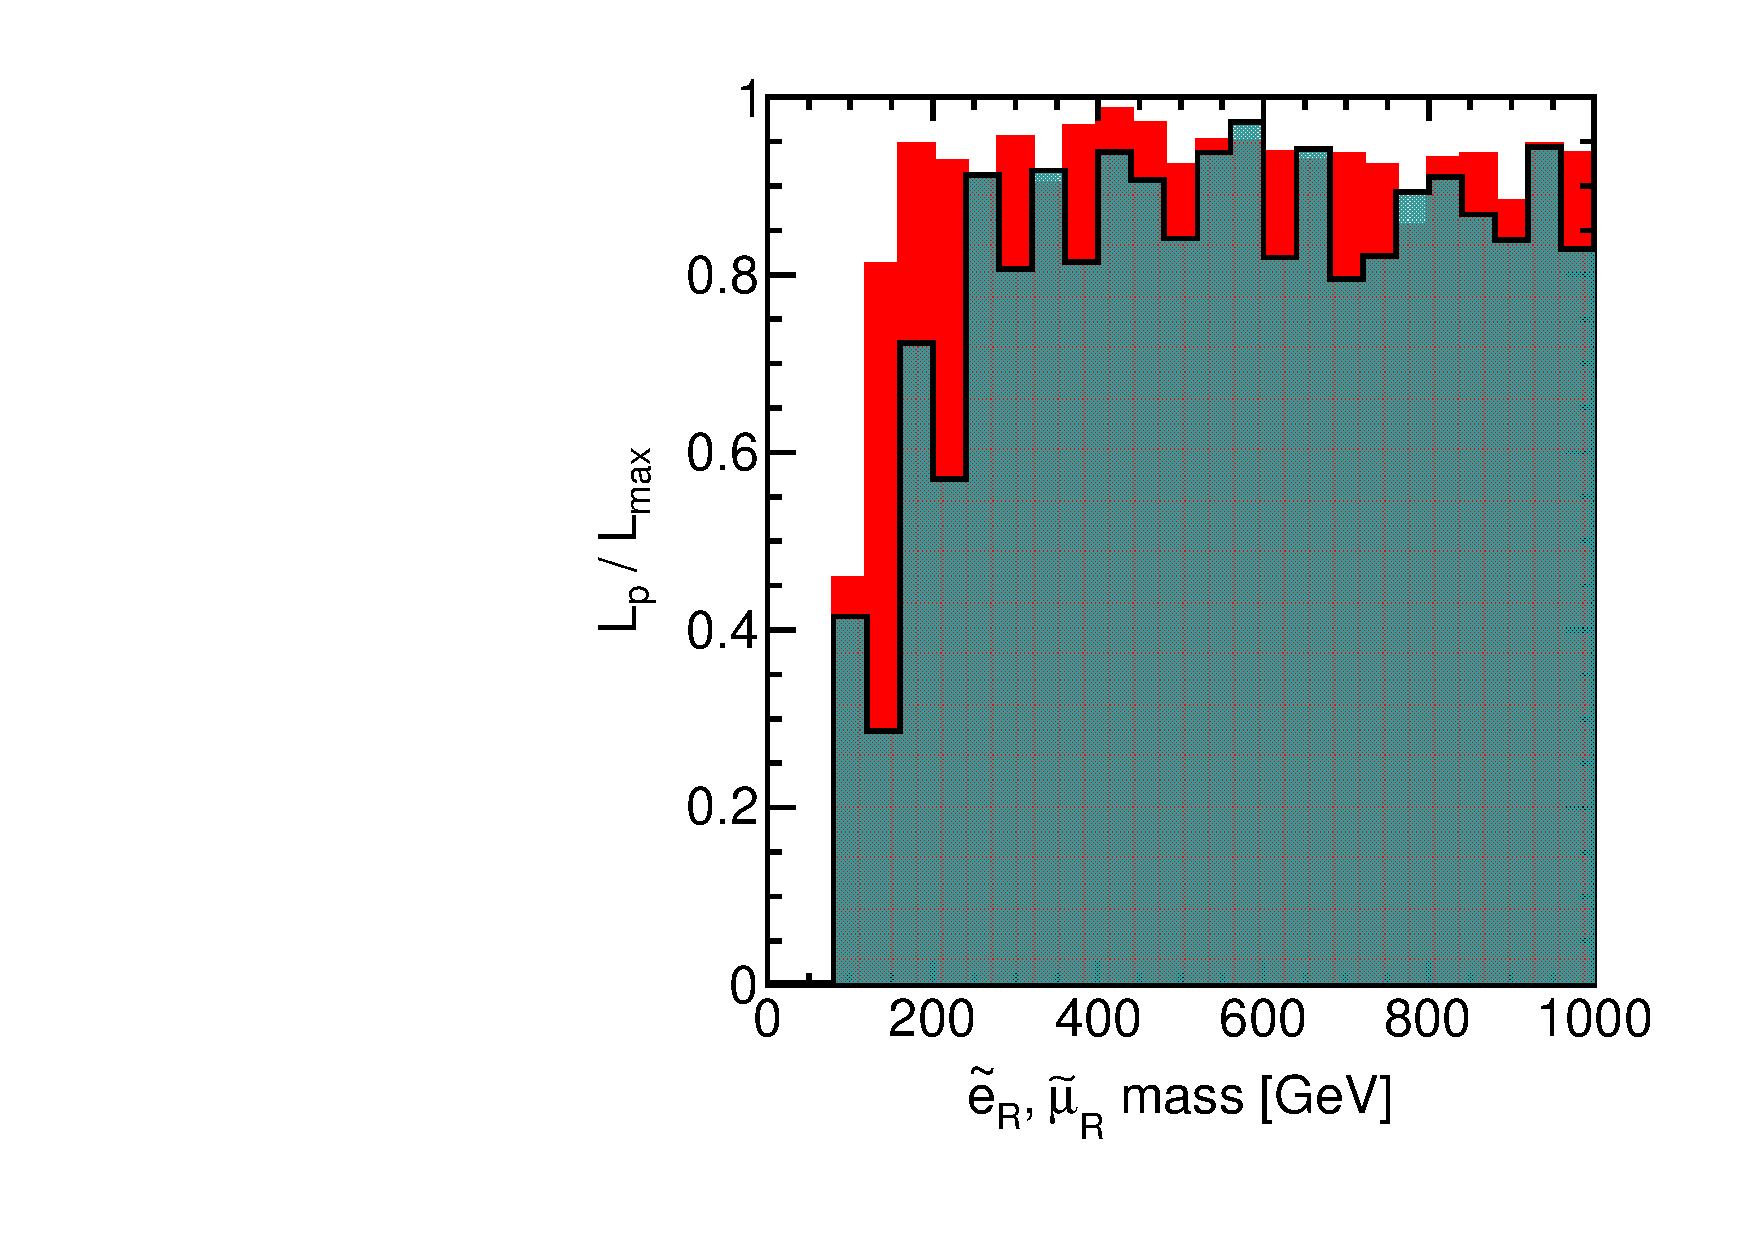
\includegraphics[height=5.5cm]{figs/fig_e_R.pdf} \\
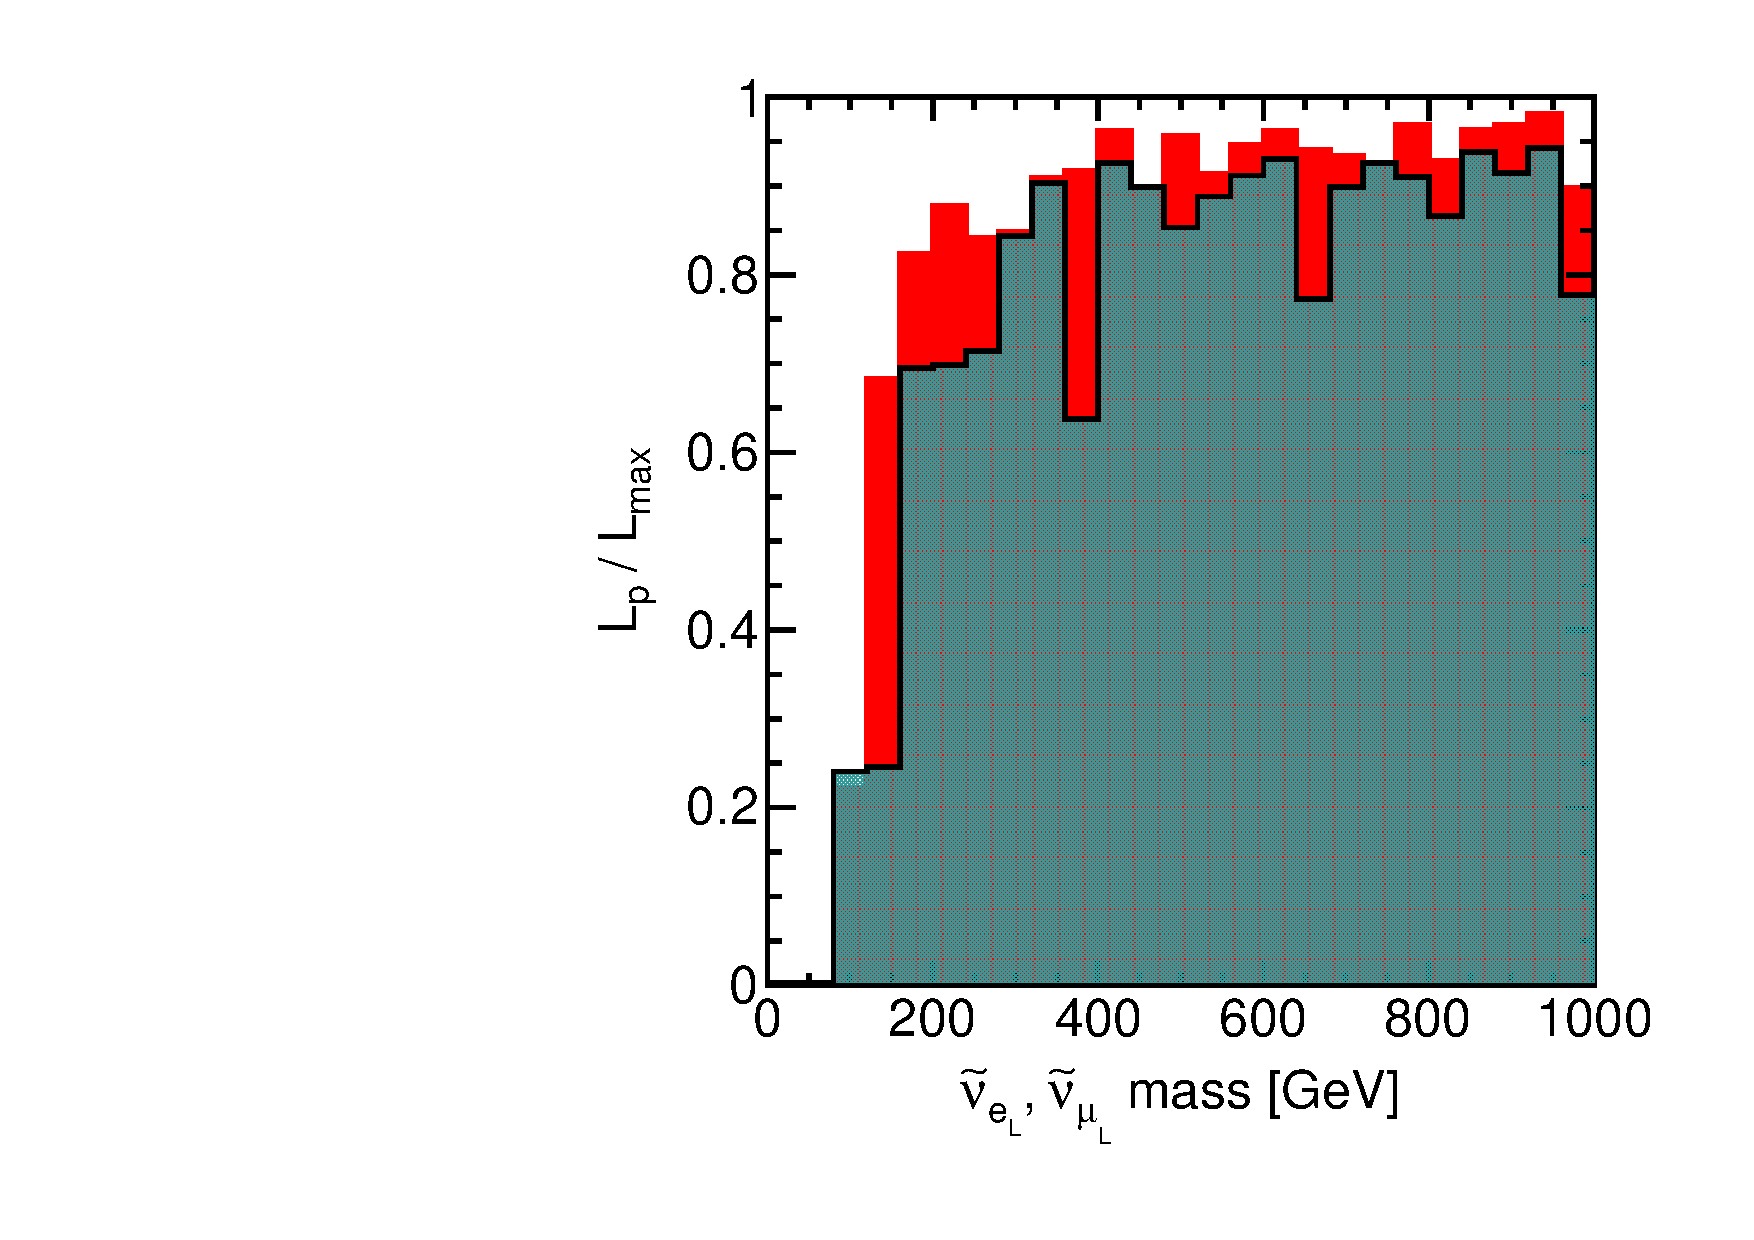
\includegraphics[height=5.5cm]{figs/fig_nu_e_L.pdf} 
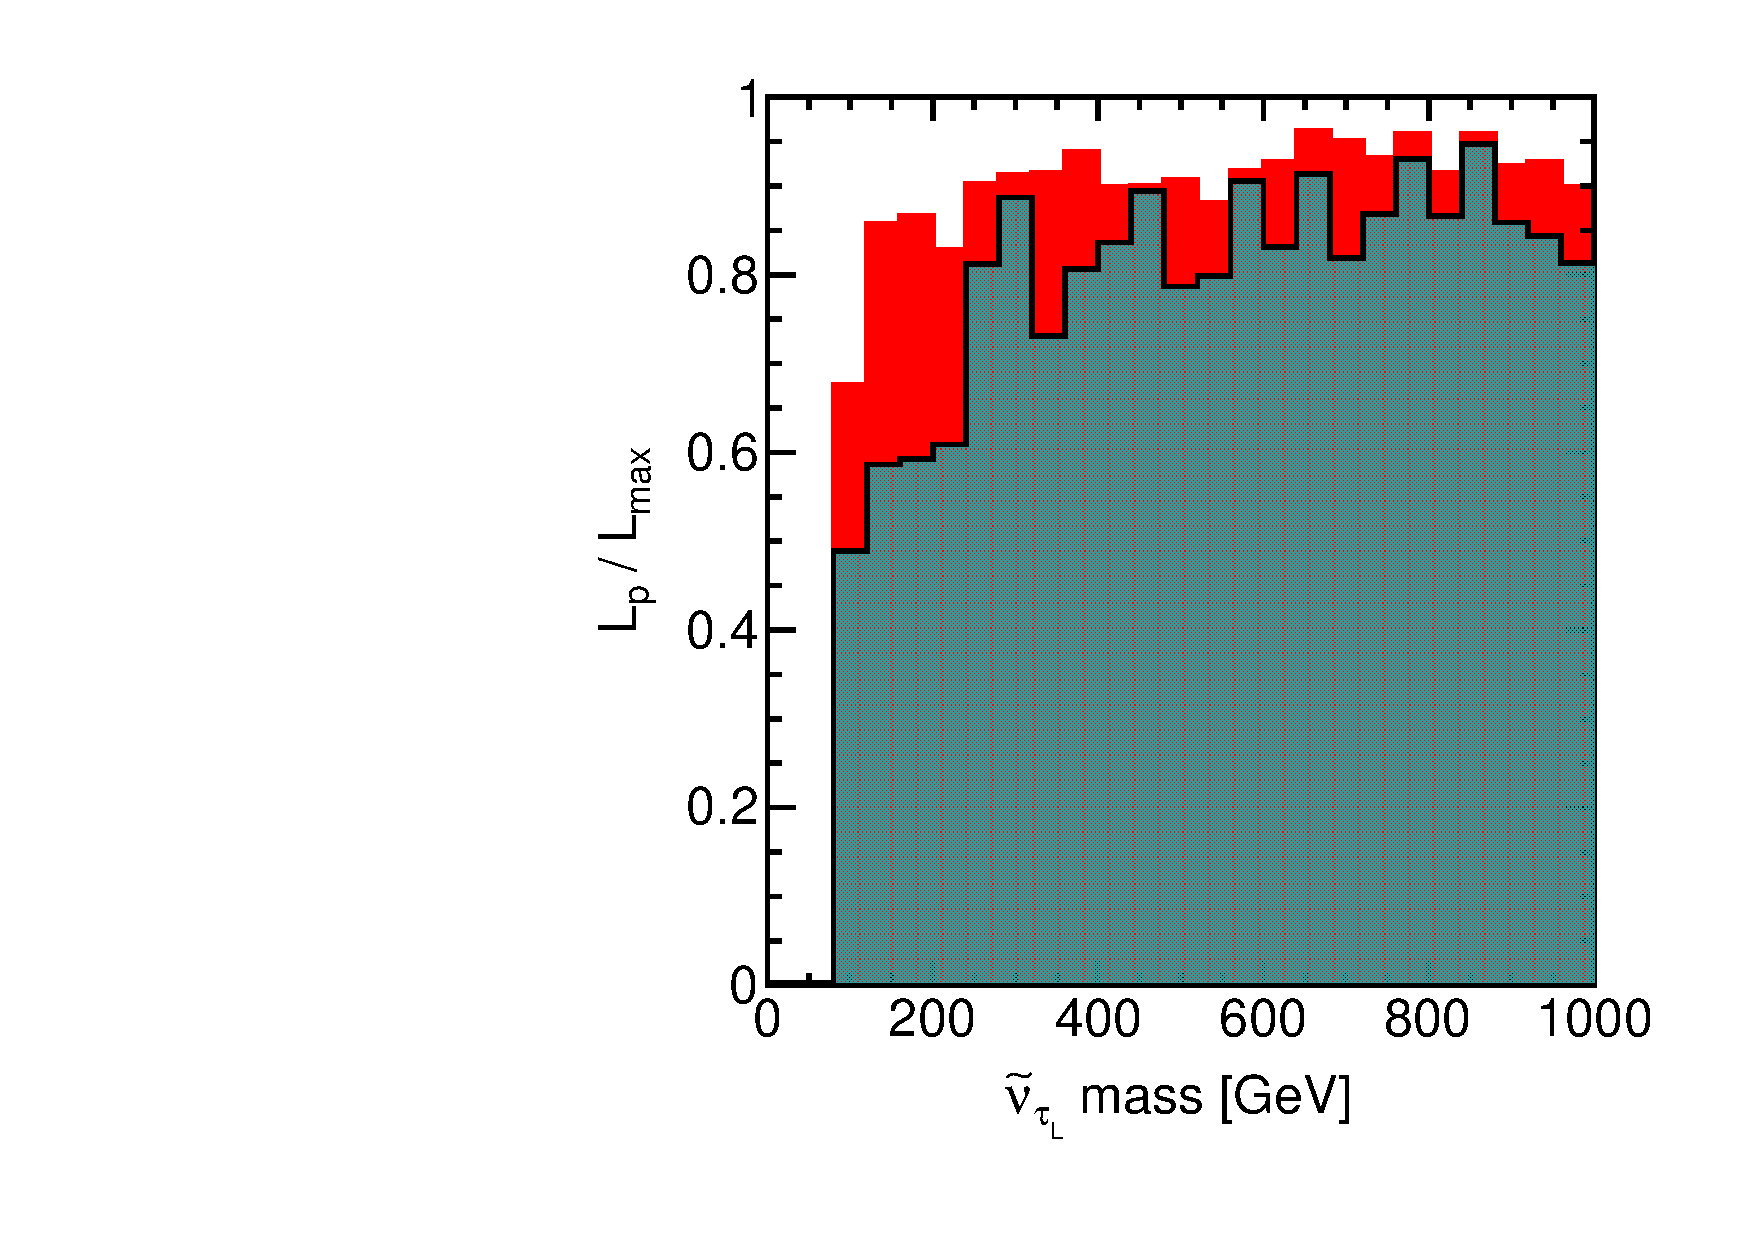
\includegraphics[height=5.5cm]{figs/fig_nu_tau_L.pdf} \\
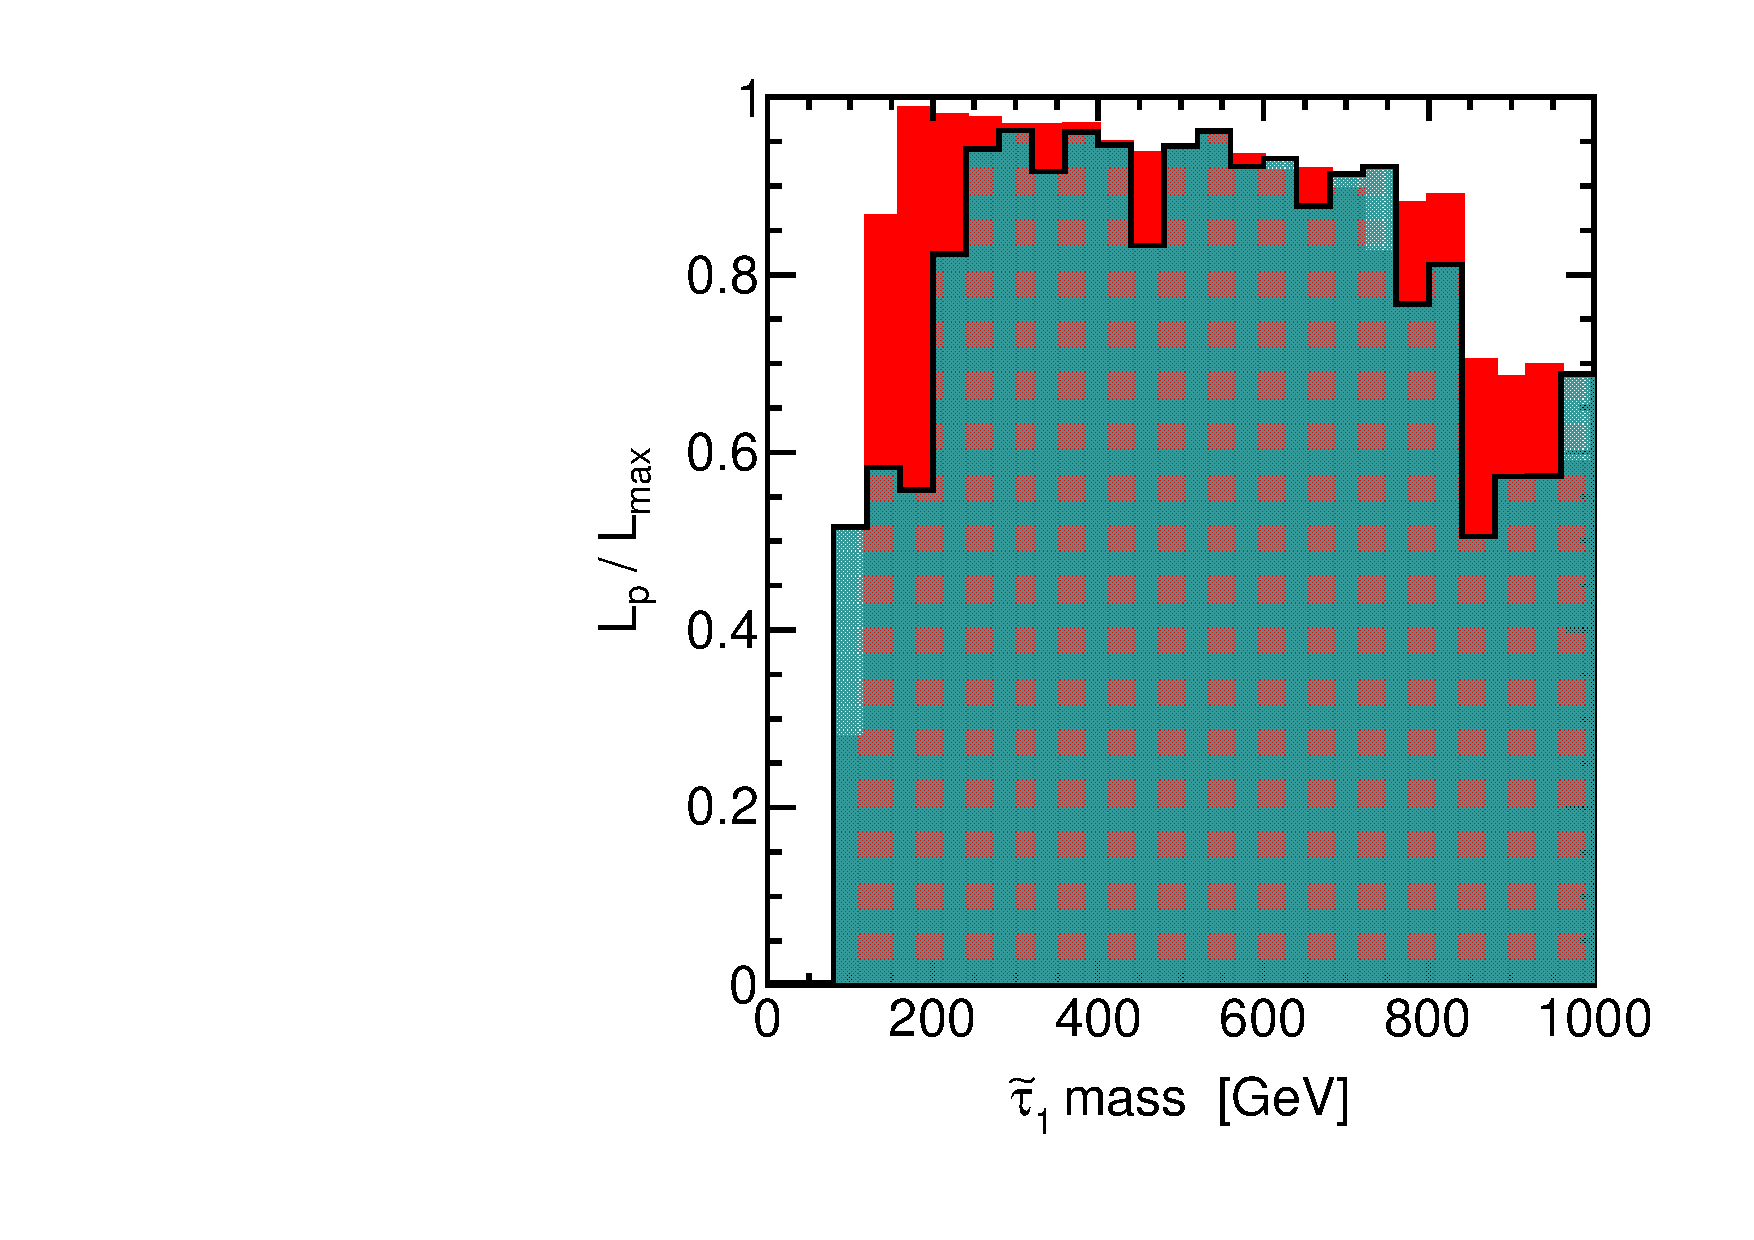
\includegraphics[height=5.5cm]{figs/fig_tau_1.pdf} 
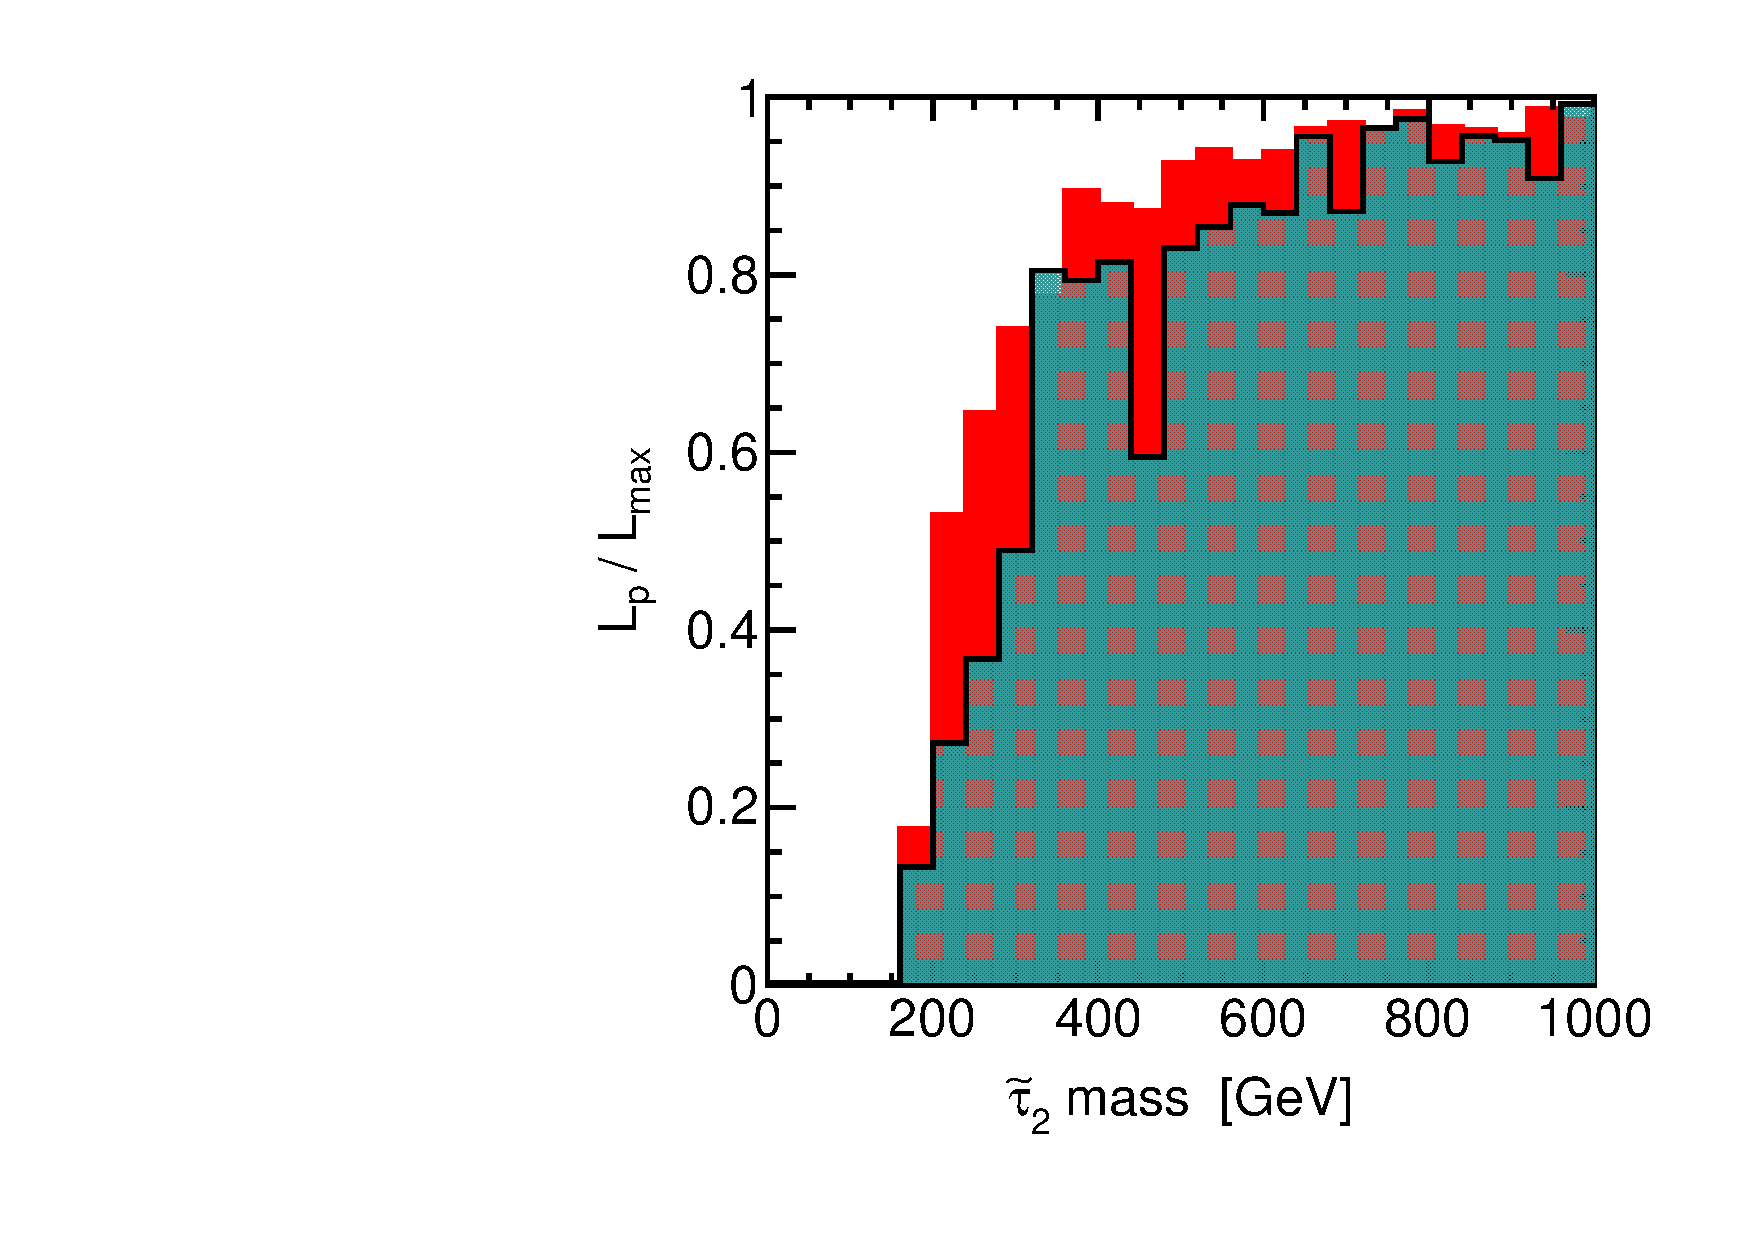
\includegraphics[height=5.5cm]{figs/fig_tau_2.pdf}
\caption{Ratios of profile likelihood $L_p$ to maximum likelihood $L_{max}$ shown for predictions for slepton masses.  The colored and shaded histograms show the distributions before and after the inclusion of the CMS results.}
\label{fig:LRwcms:sl}
\end{center}
\end{figure}

\begin{figure}[htbp]
\begin{center}
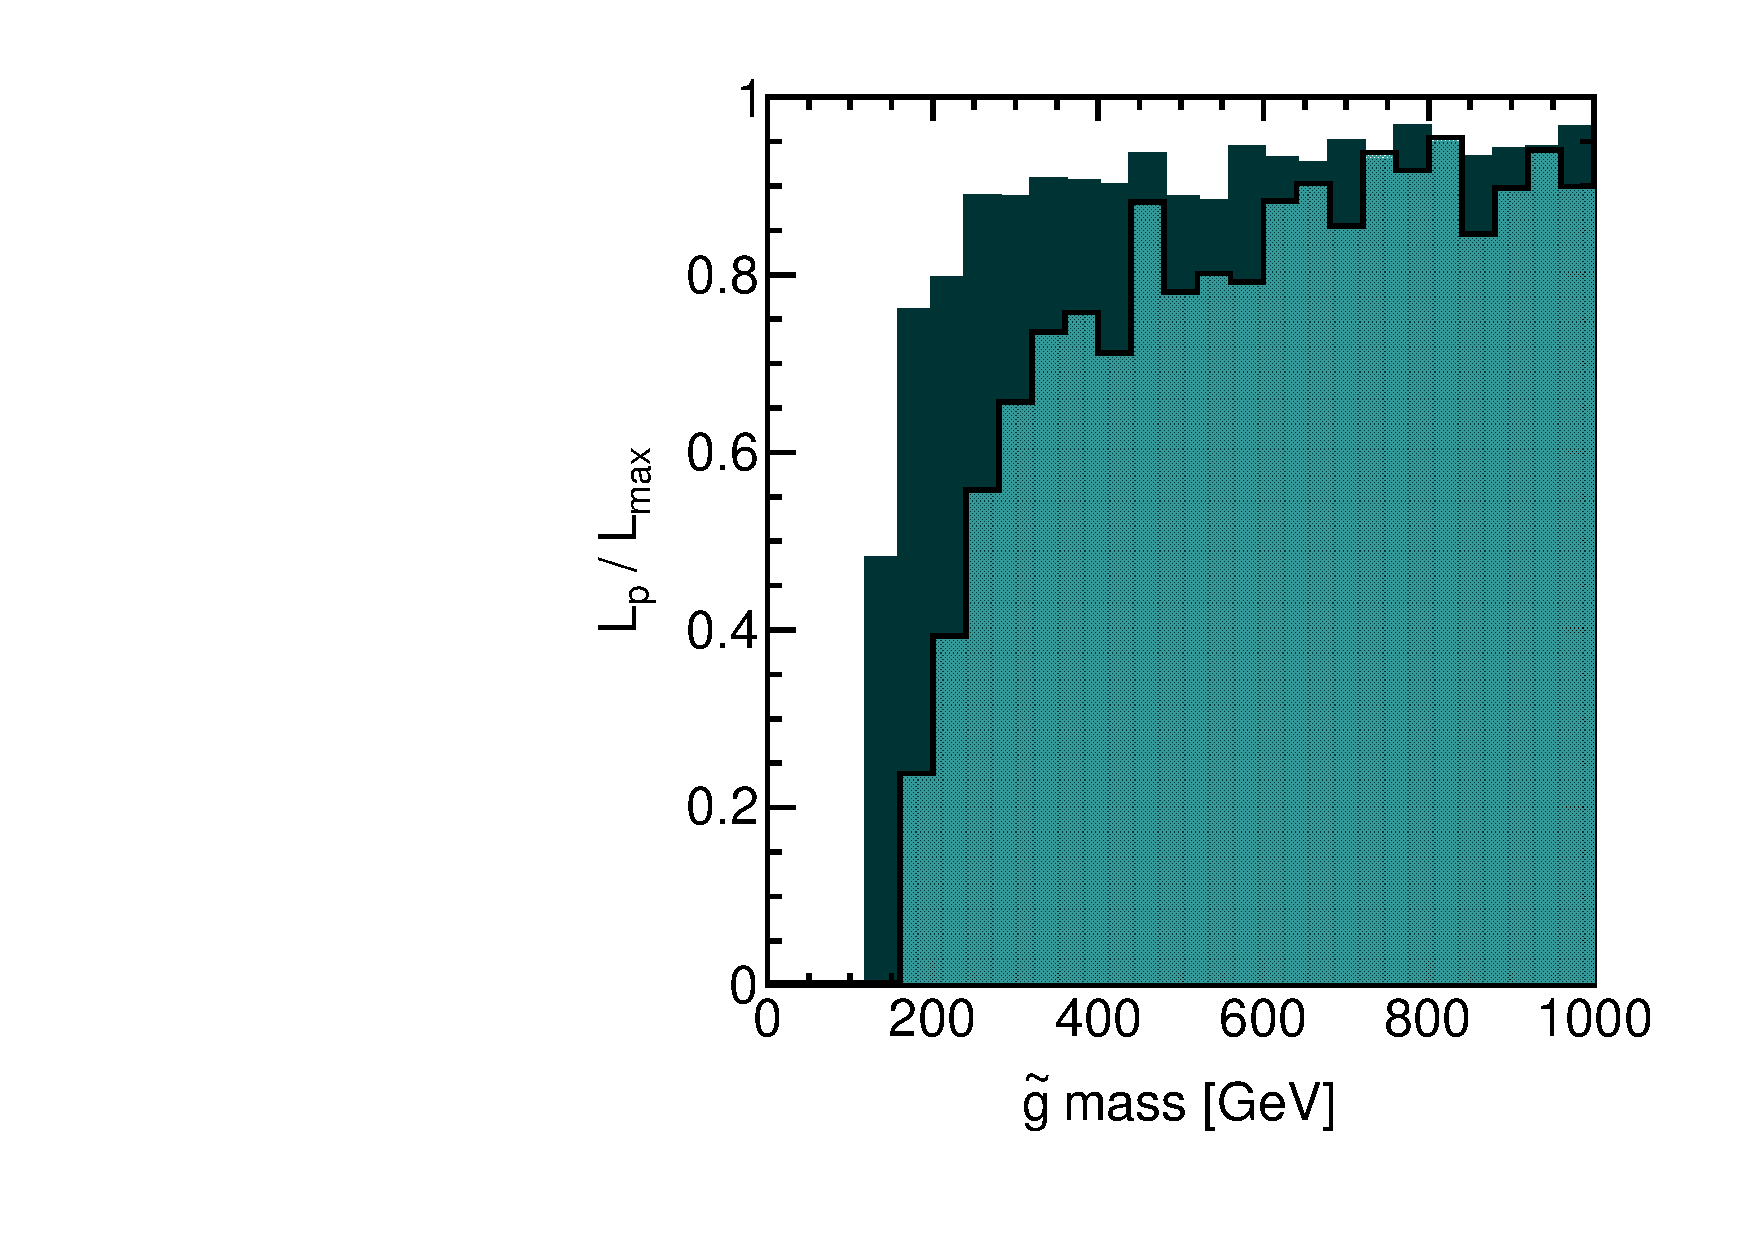
\includegraphics[height=5.5cm]{figs/fig_g.pdf} 
\caption{Ratios of profile likelihood $L_p$ to maximum likelihood $L_{max}$ shown for the gluino mass.  The colored and shaded histograms show the distributions before and after the inclusion of the CMS results.}
\label{fig:LRwcms:g}
\end{center}
\end{figure}


\begin{figure}[htbp]
\begin{center}
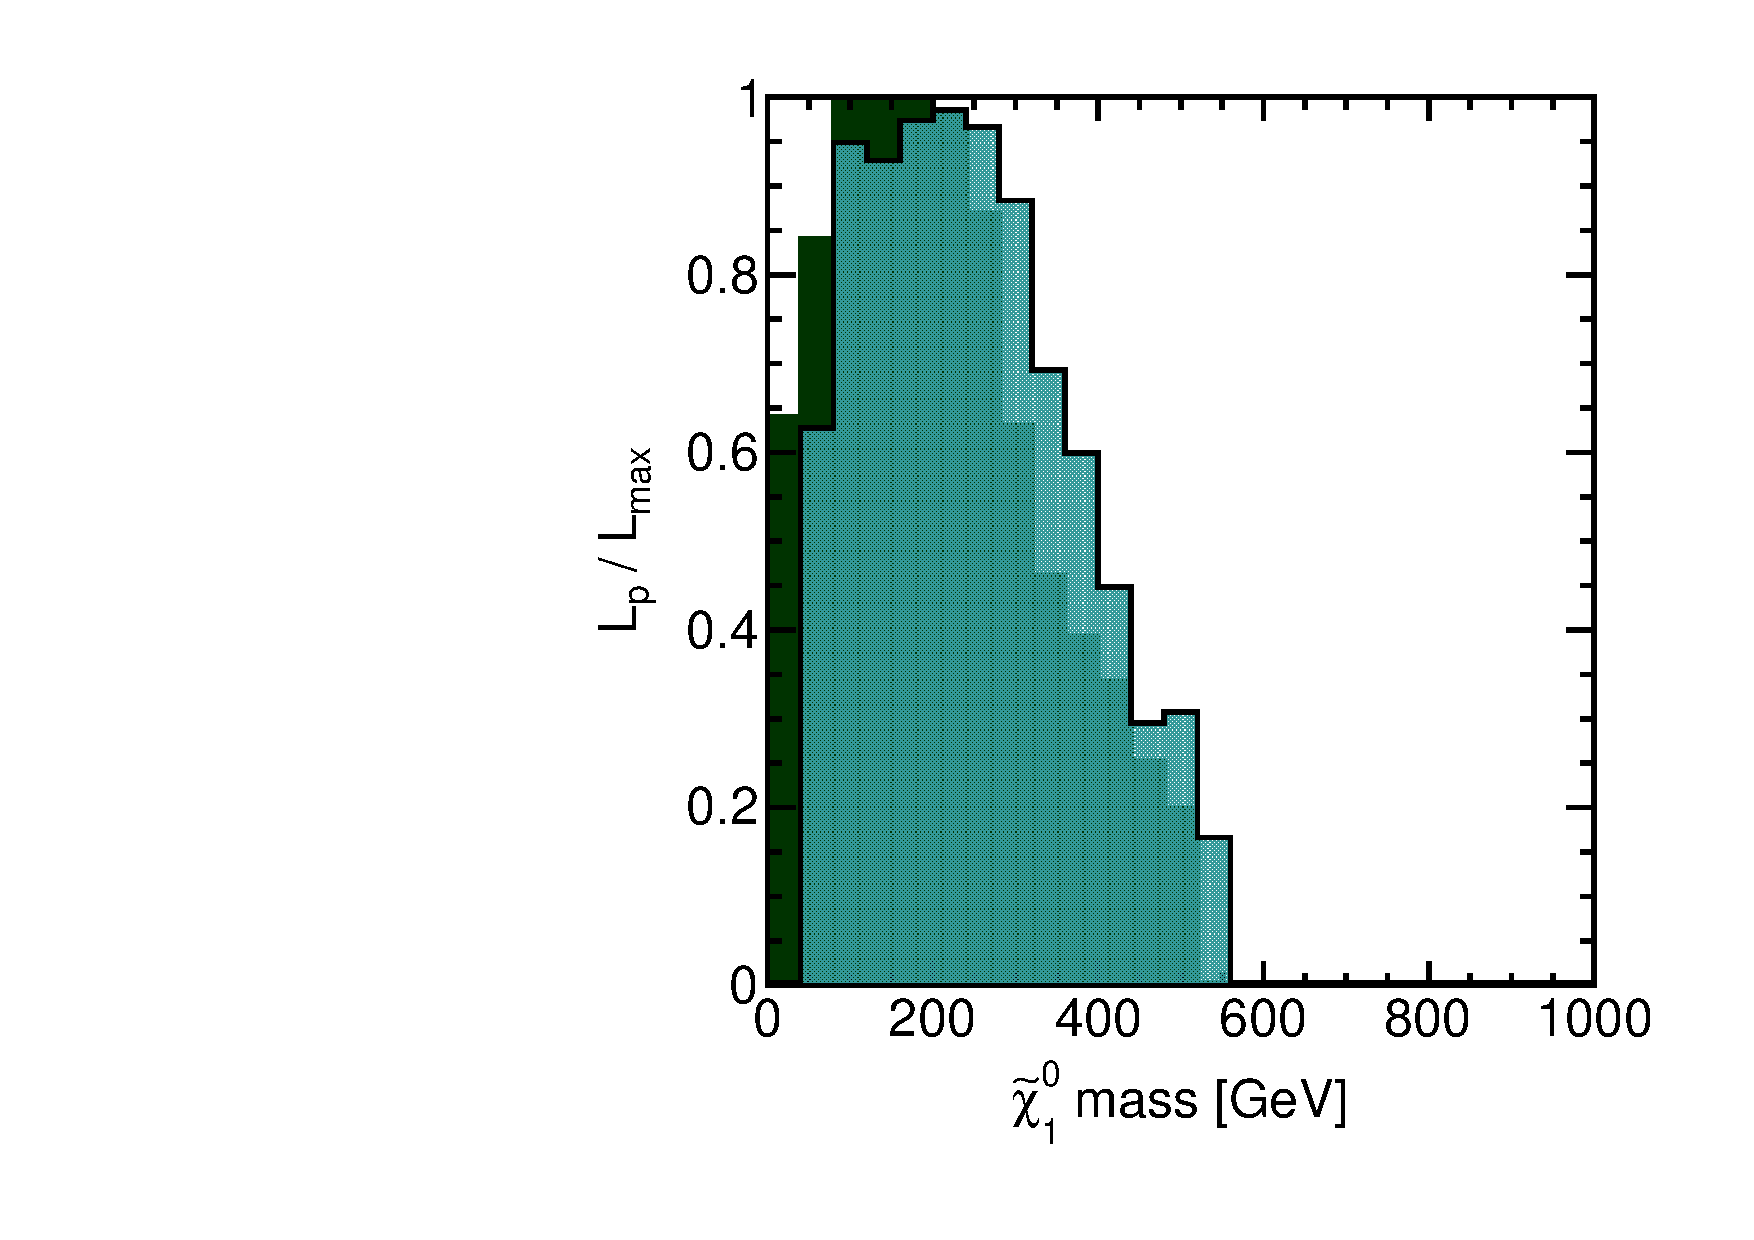
\includegraphics[height=5.5cm]{figs/fig_chi_1_0.pdf} 
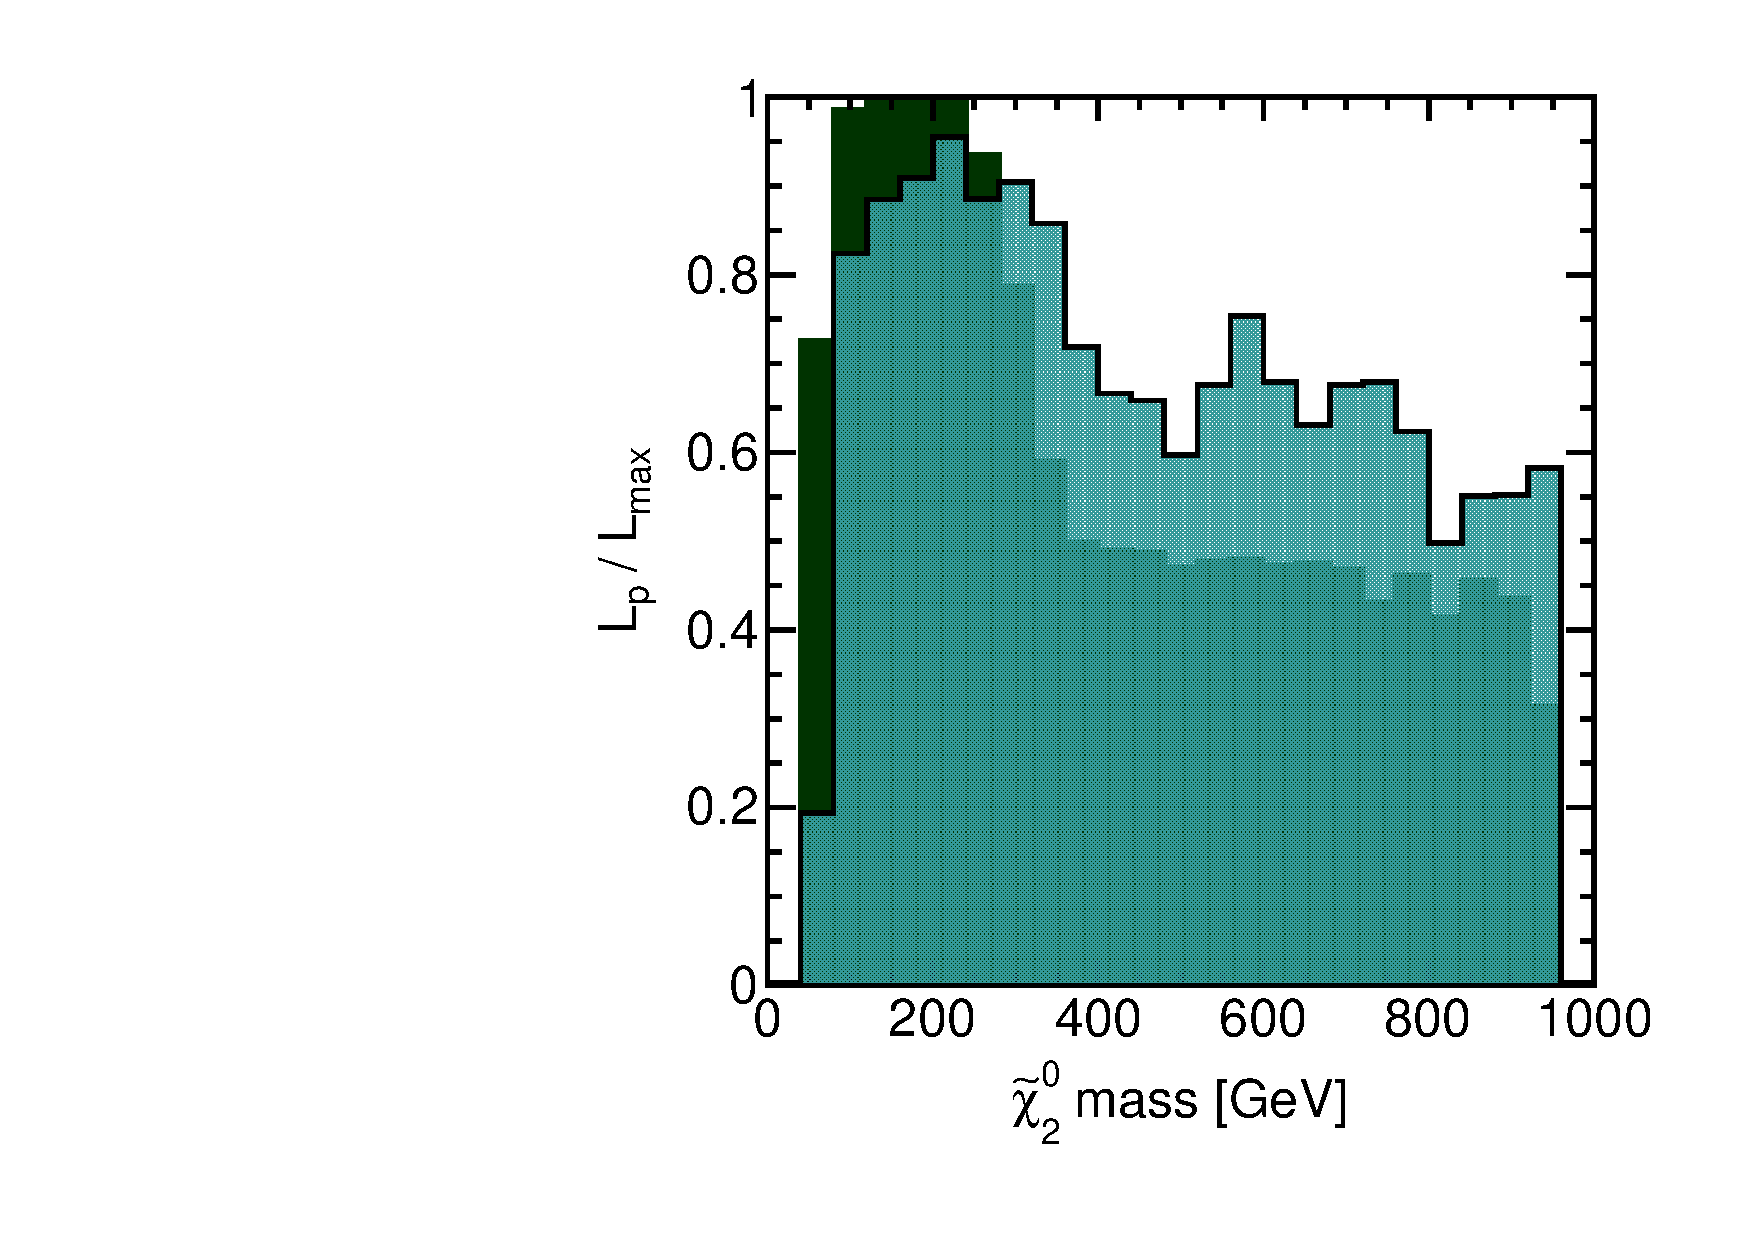
\includegraphics[height=5.5cm]{figs/fig_chi_2_0.pdf} \\
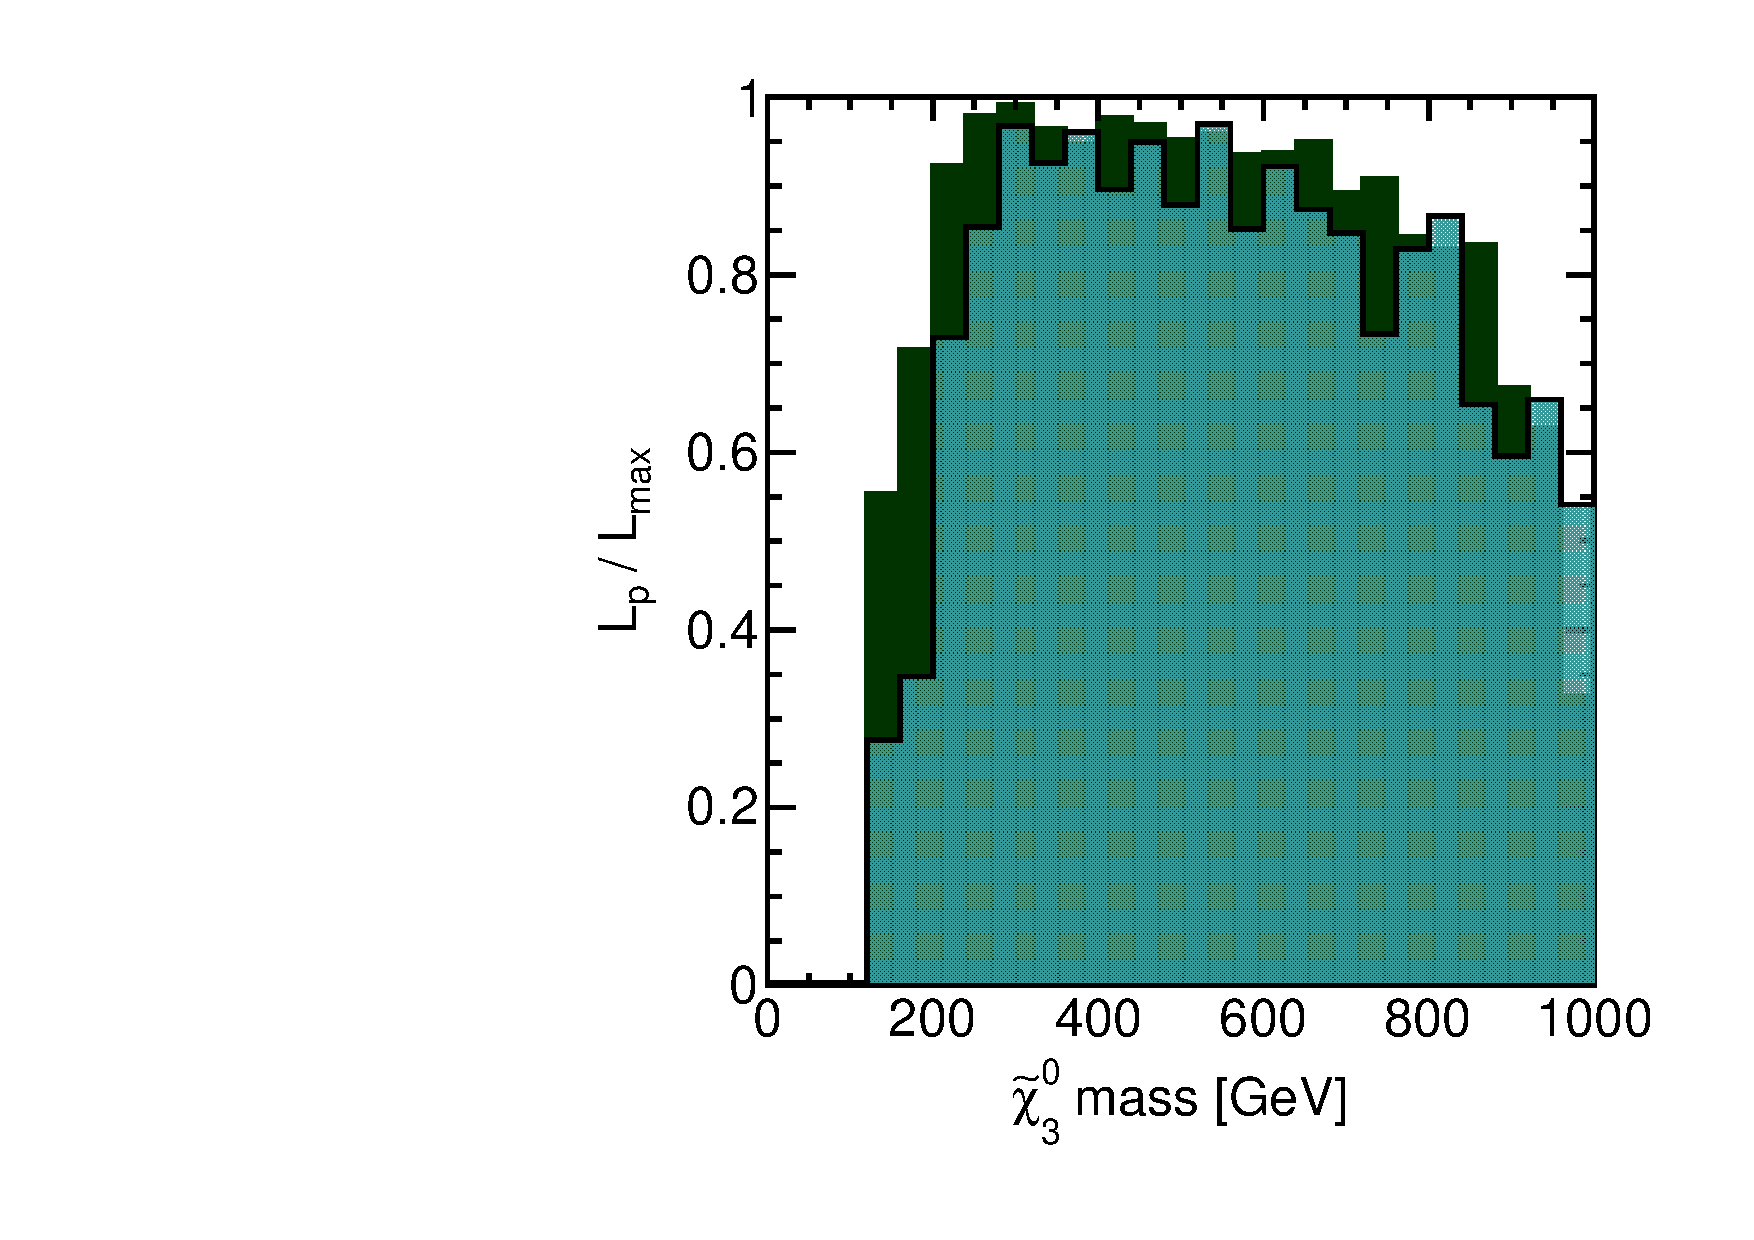
\includegraphics[height=5.5cm]{figs/fig_chi_3_0.pdf} 
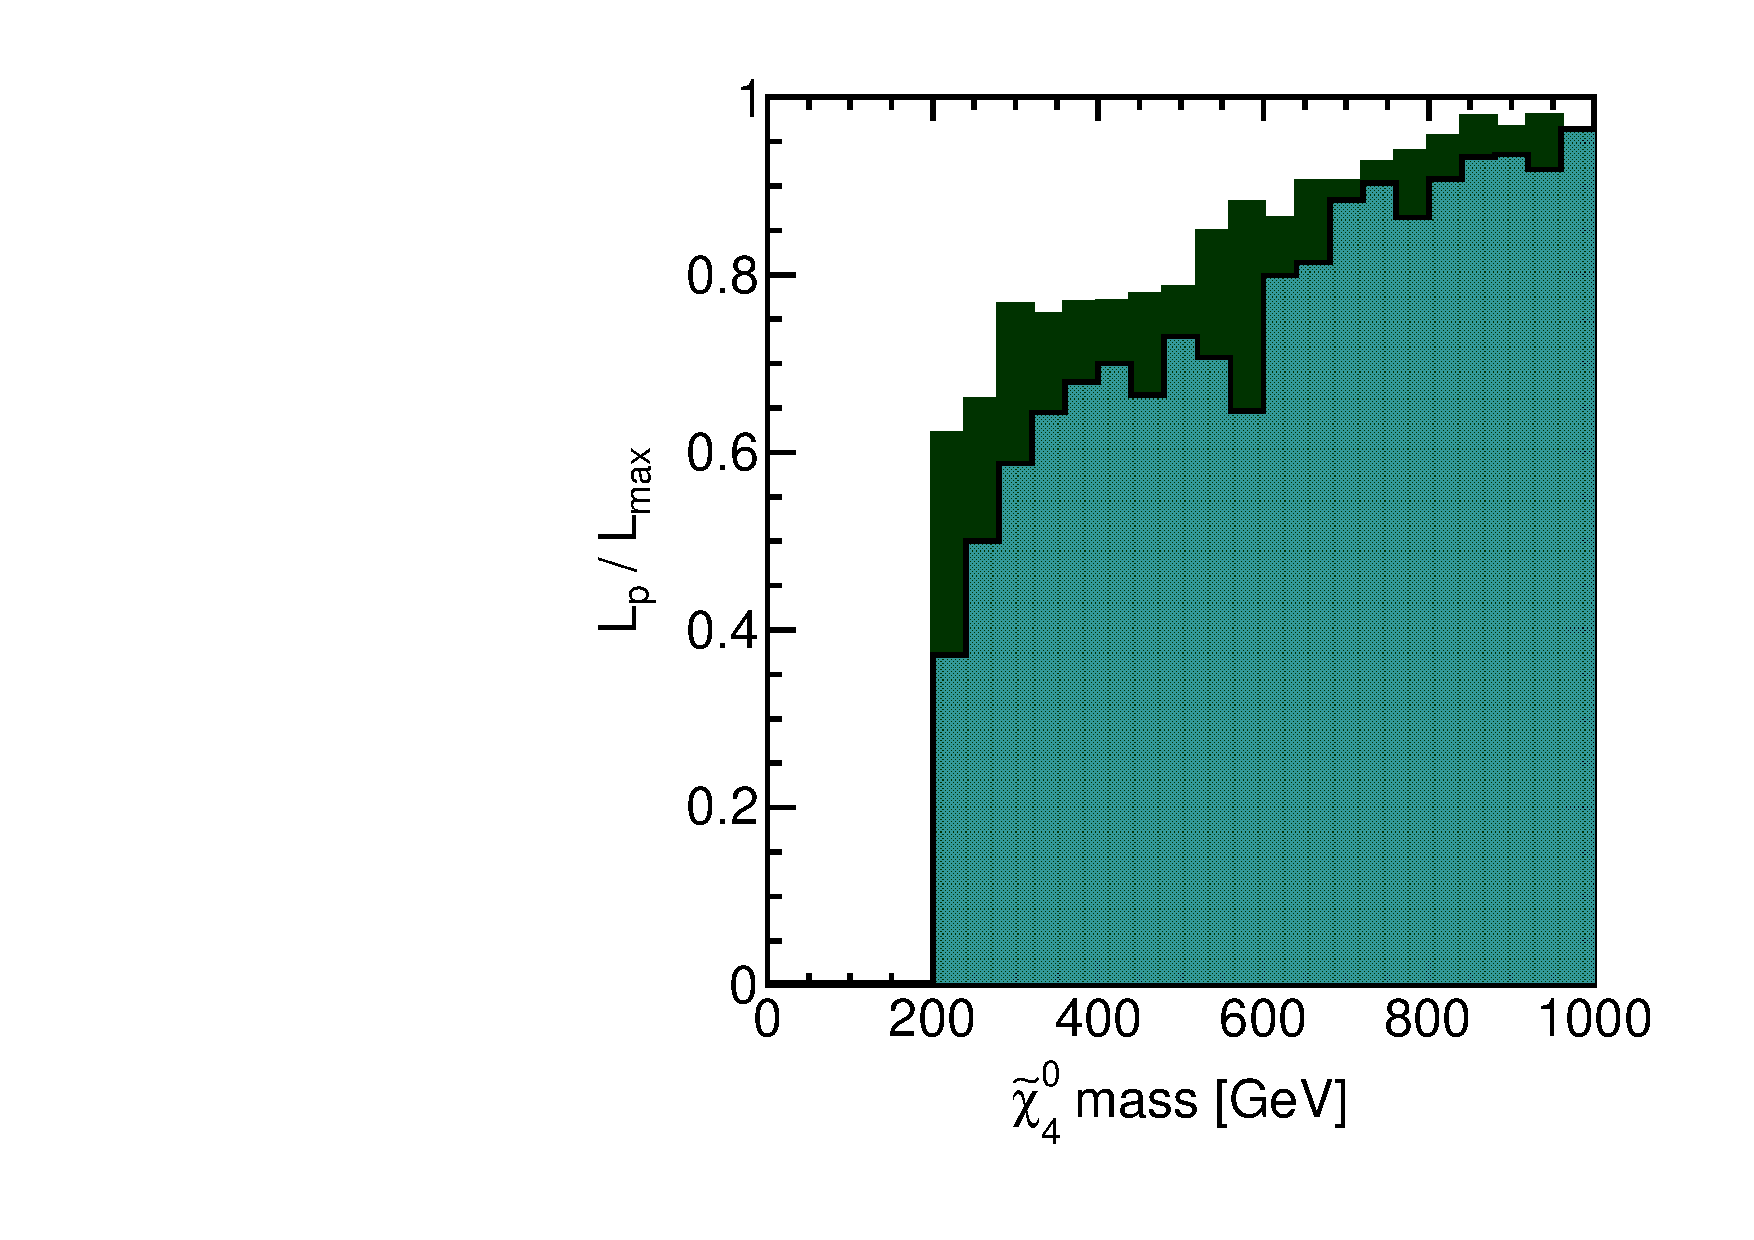
\includegraphics[height=5.5cm]{figs/fig_chi_4_0.pdf} 
\caption{Ratios of profile likelihood $L_p$ to maximum likelihood $L_{max}$ shown for the neutralino masses.  The colored and shaded histograms show the distributions before and after the inclusion of the CMS results.}
\label{fig:LRwcms_chi0}
\end{center}
\end{figure}

\begin{figure}[htbp]
\begin{center}
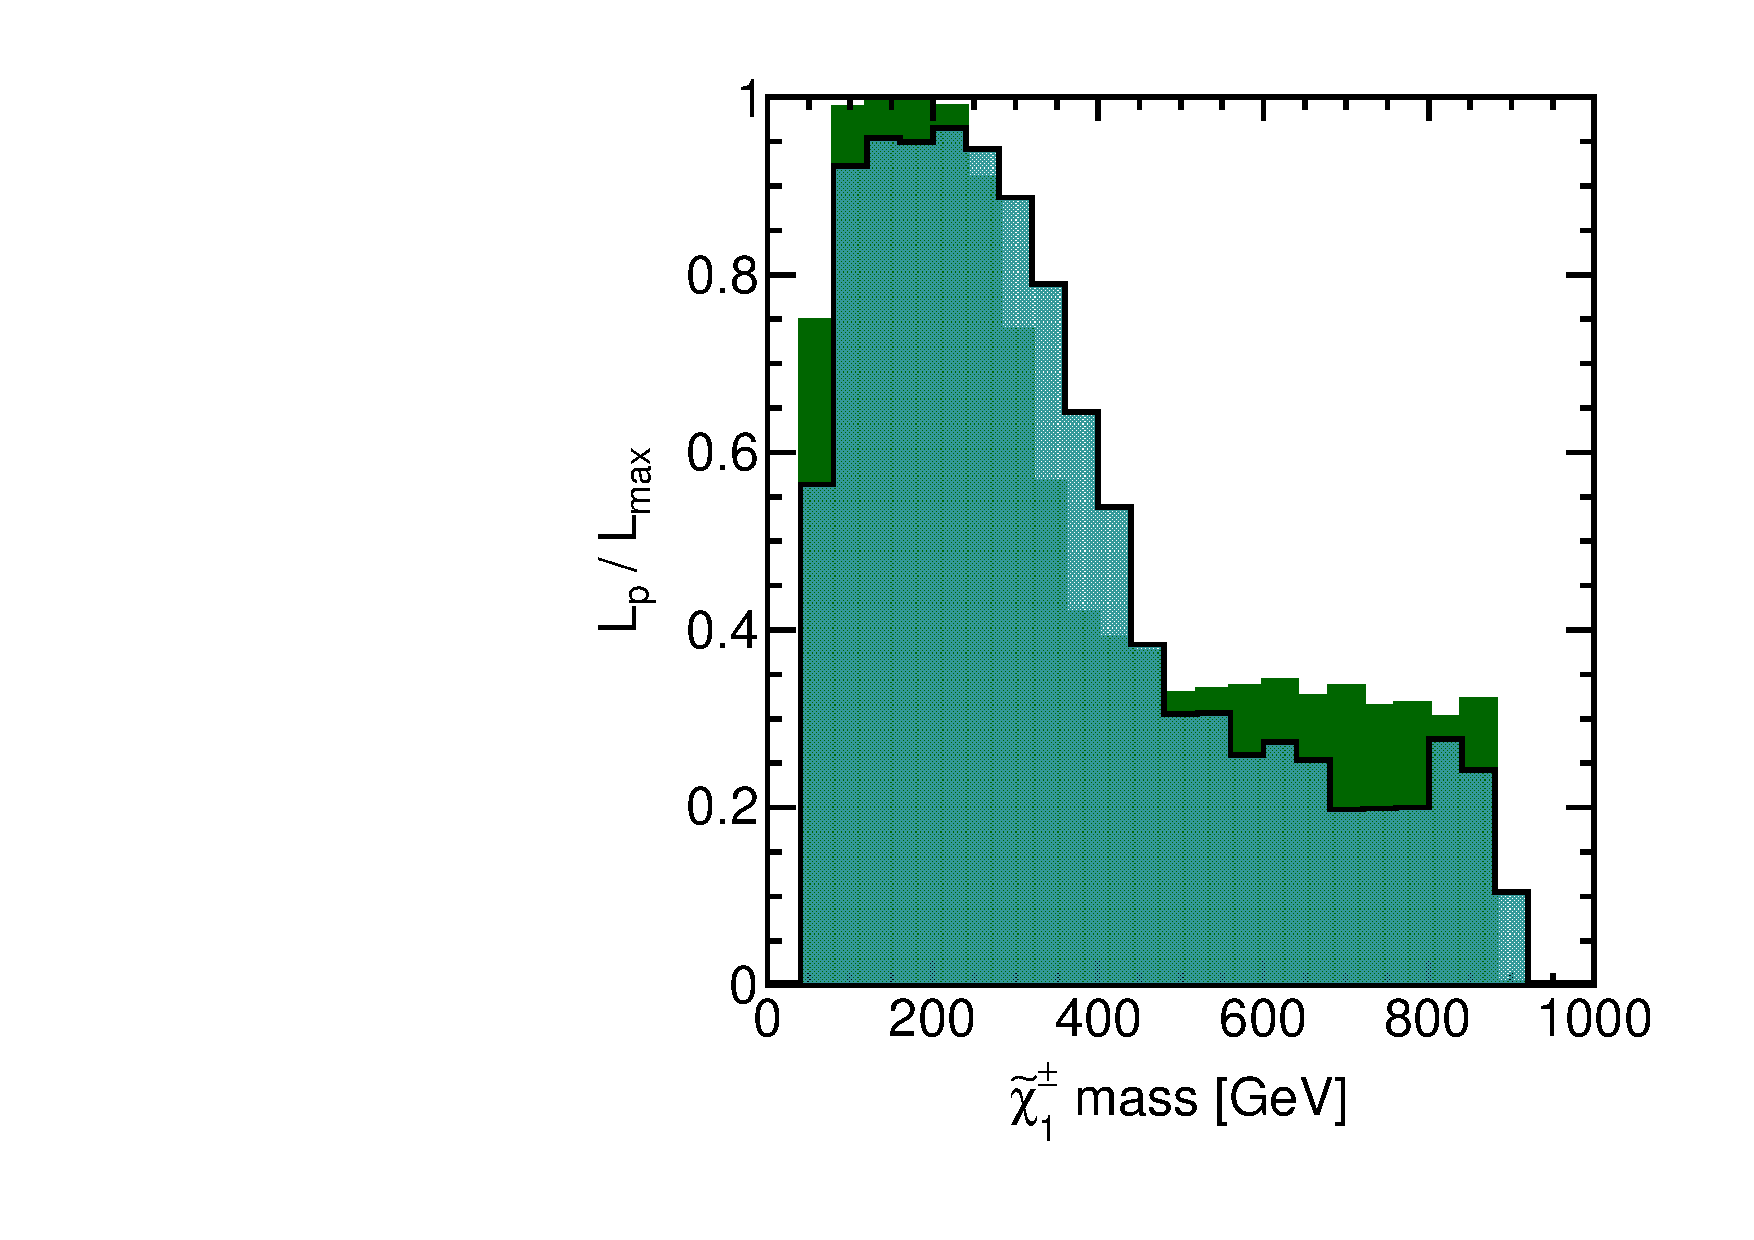
\includegraphics[height=5.5cm]{figs/fig_chi_1_pm.pdf} 
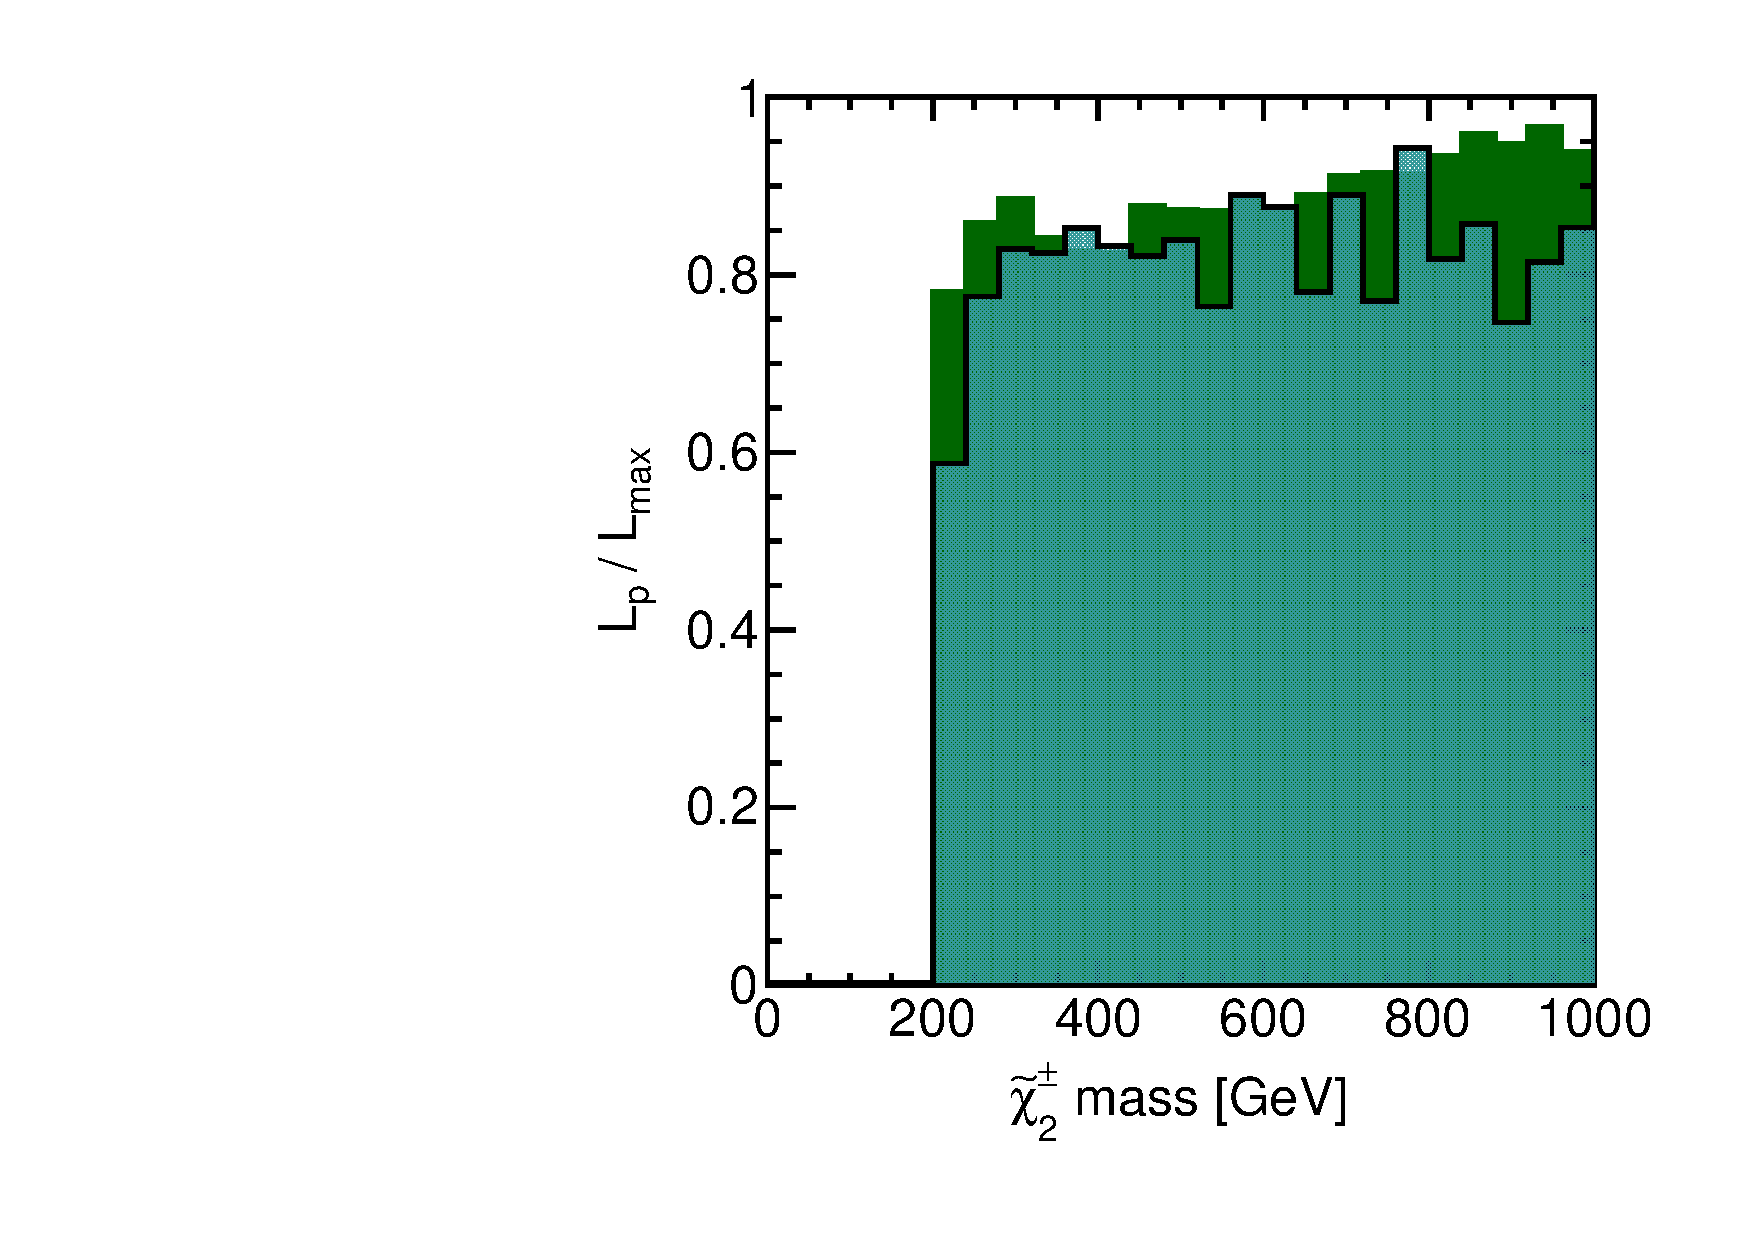
\includegraphics[height=5.5cm]{figs/fig_chi_2_pm.pdf}
\caption{Ratios of profile likelihood $L_p$ to maximum likelihood $L_{max}$ shown for chargino masses.  The colored and shaded histograms show the distributions before and after the inclusion of the CMS results.}
\label{fig:LRwcms_chipm}
\end{center}
\end{figure}


\begin{figure}[htbp]
\begin{center}
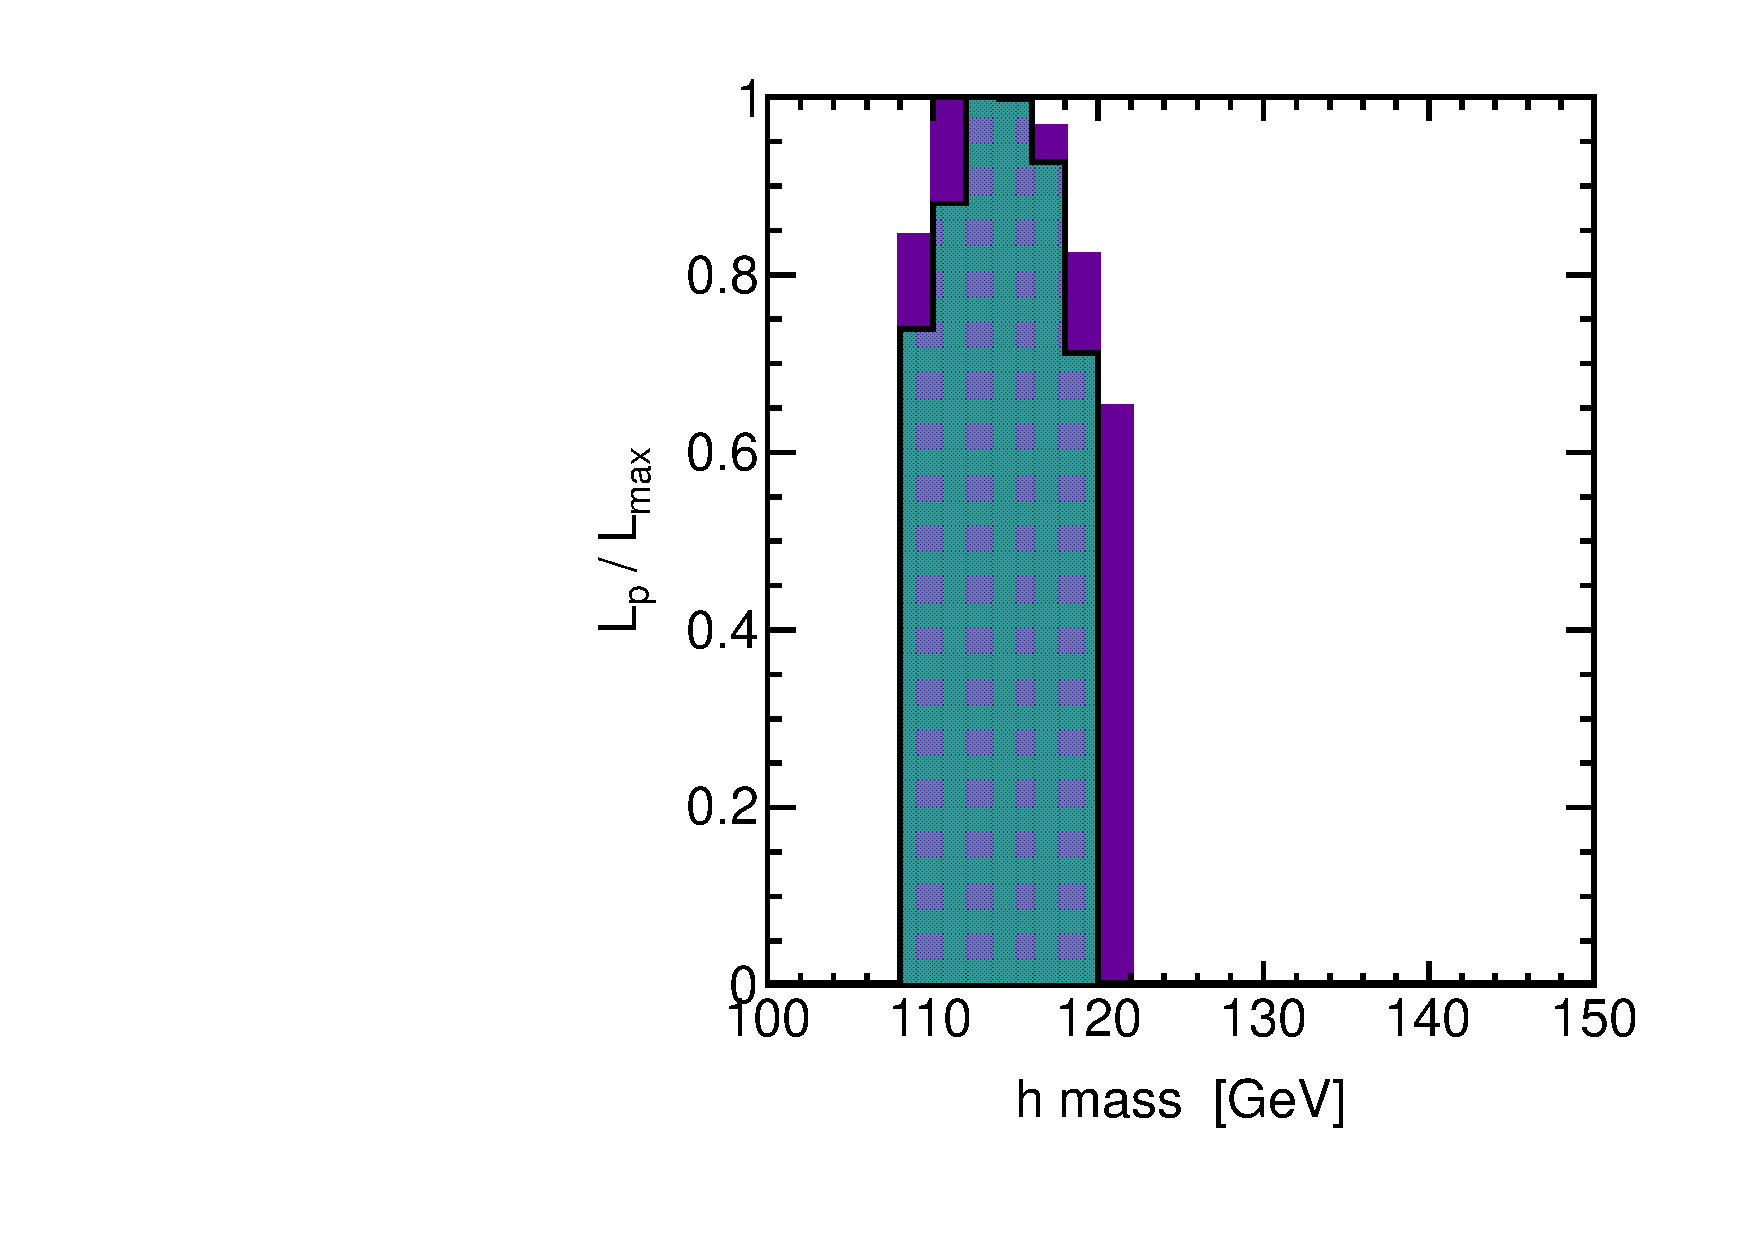
\includegraphics[height=5.5cm]{figs/fig_h.pdf} 
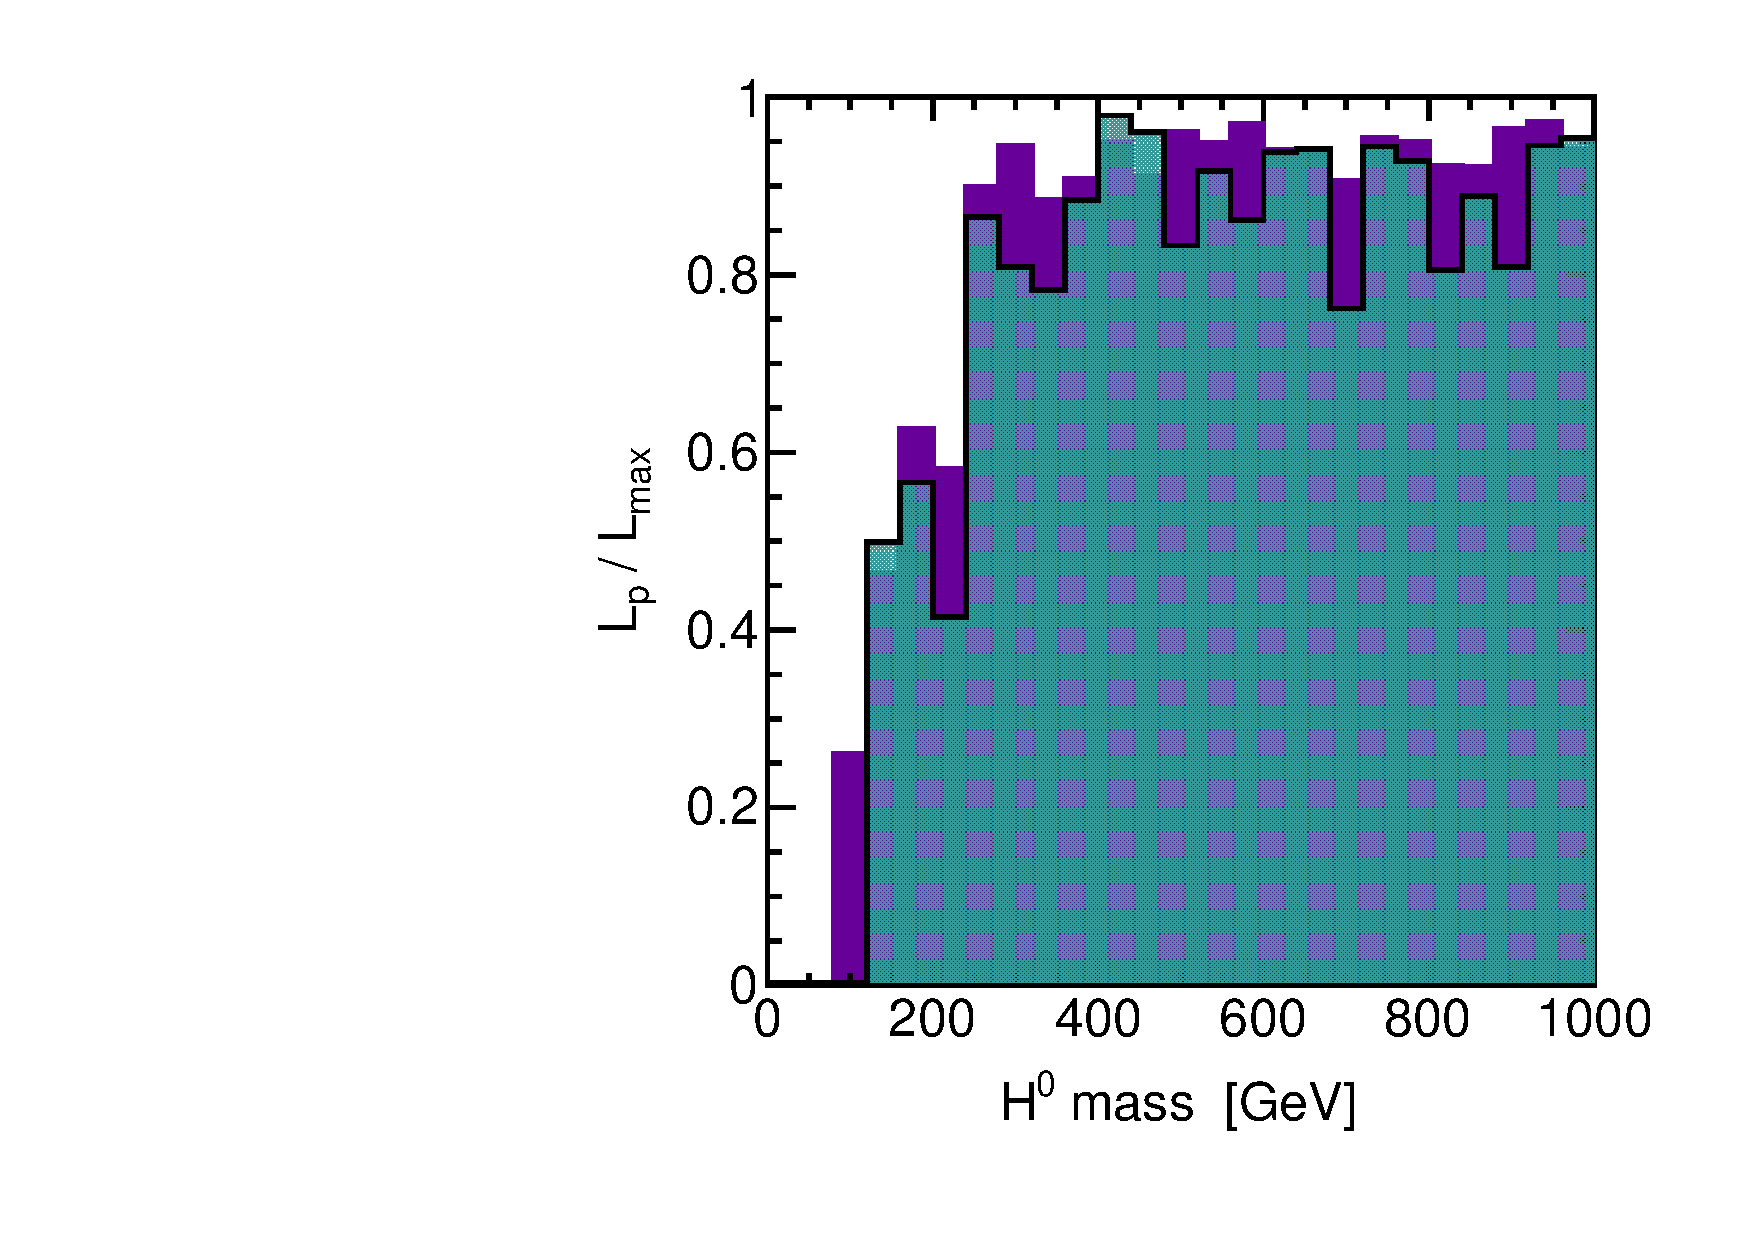
\includegraphics[height=5.5cm]{figs/fig_H0.pdf} \\
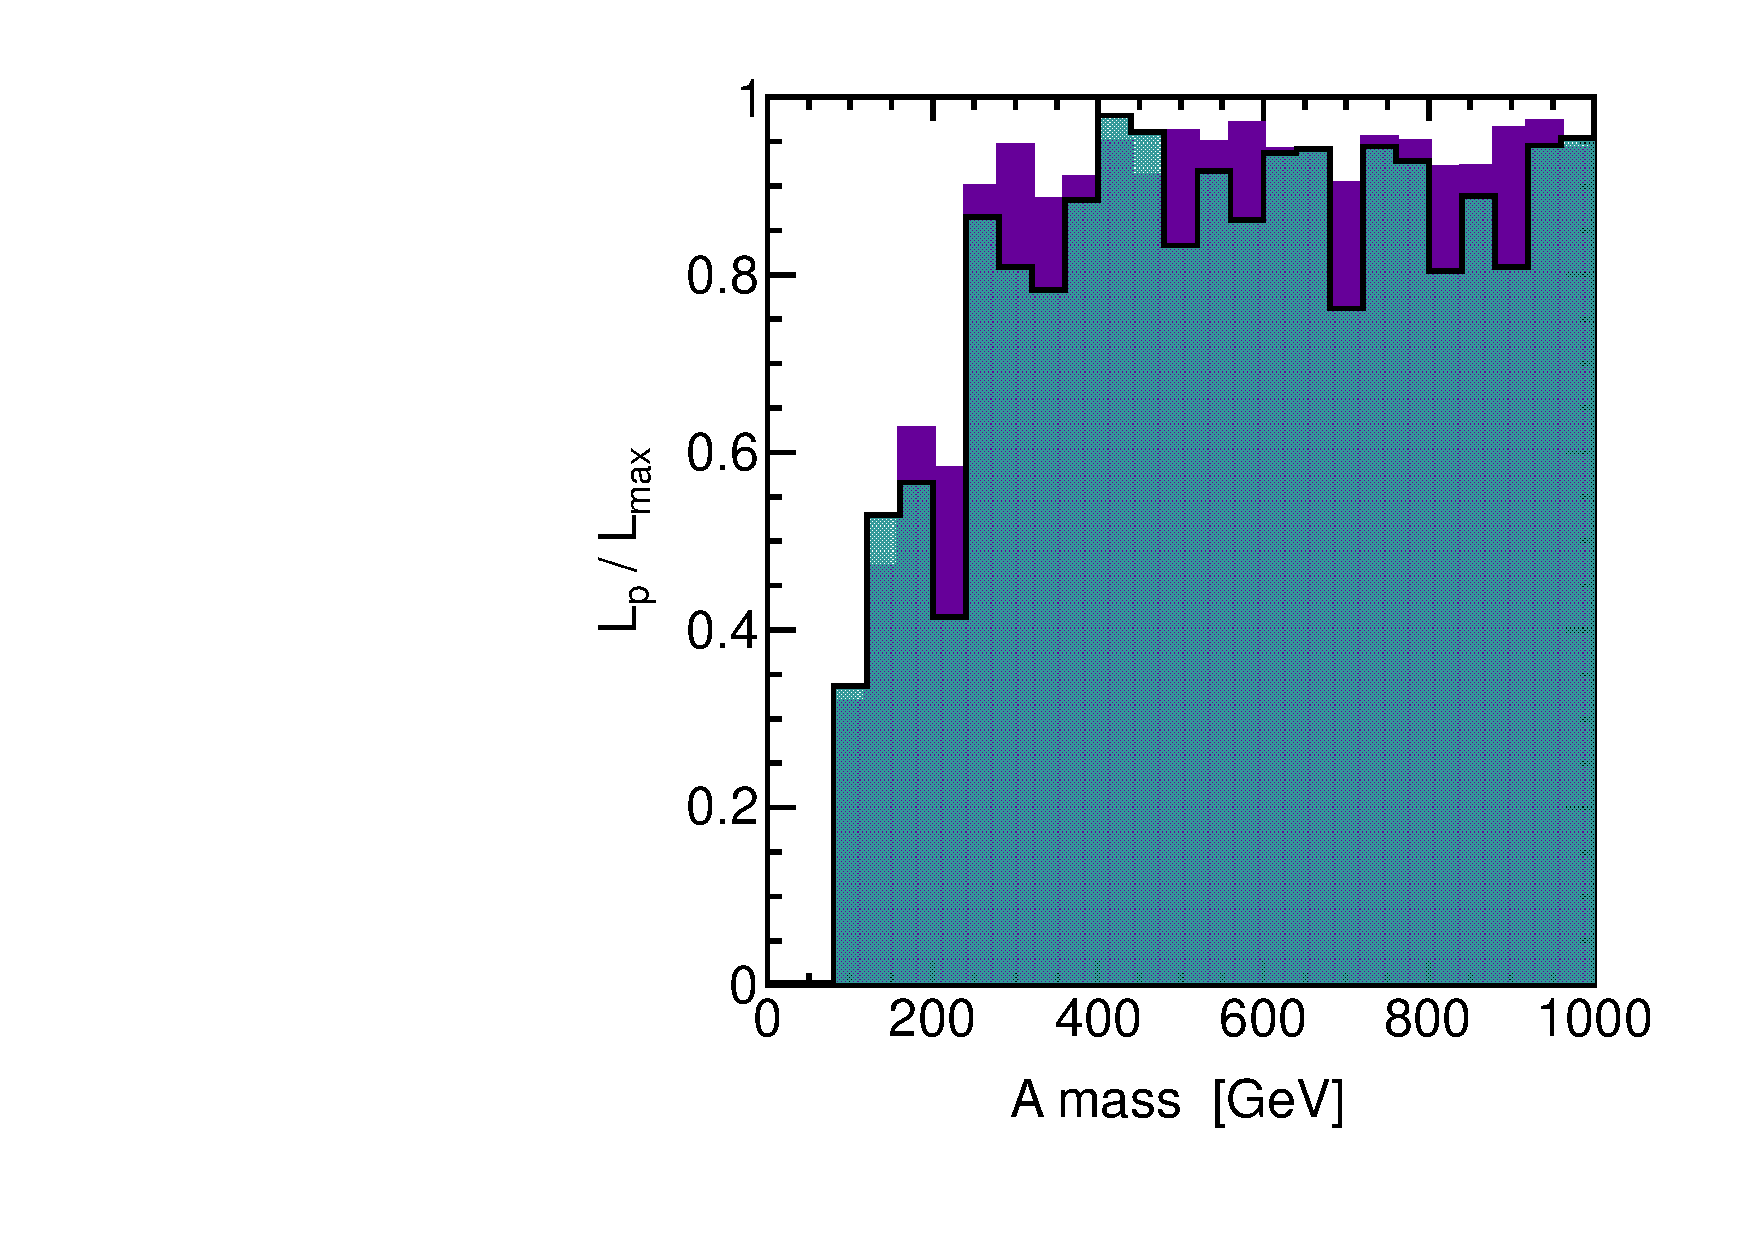
\includegraphics[height=5.5cm]{figs/fig_A.pdf} 
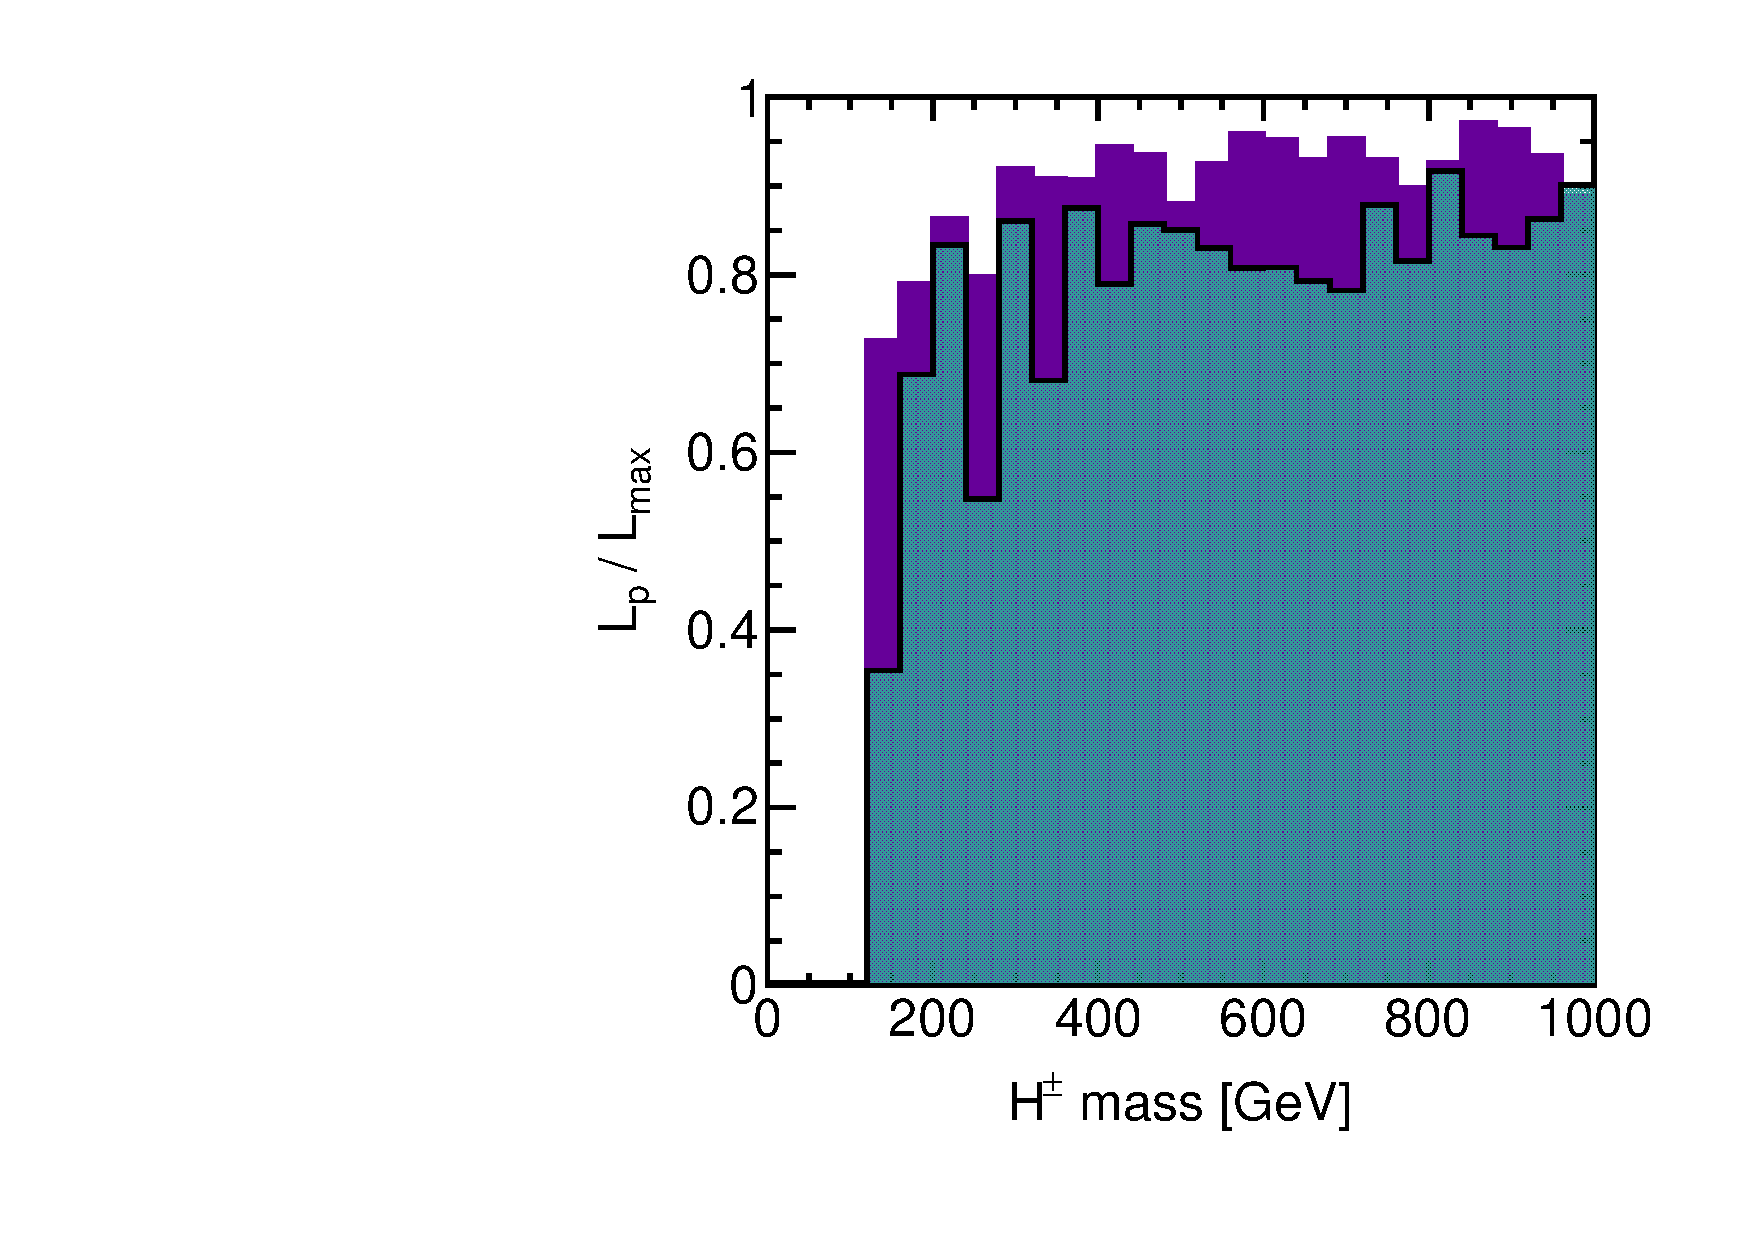
\includegraphics[height=5.5cm]{figs/fig_H_pm.pdf} 
\caption{Ratios of profile likelihood $L_p$ to maximum likelihood $L_{max}$ shown for the Higgs masses.  The colored and shaded histograms show the distributions before and after the inclusion of the CMS results.}
\label{fig:LRwcms_Higgs}
\end{center}
\end{figure}


\begin{figure}[htbp]
\begin{center}
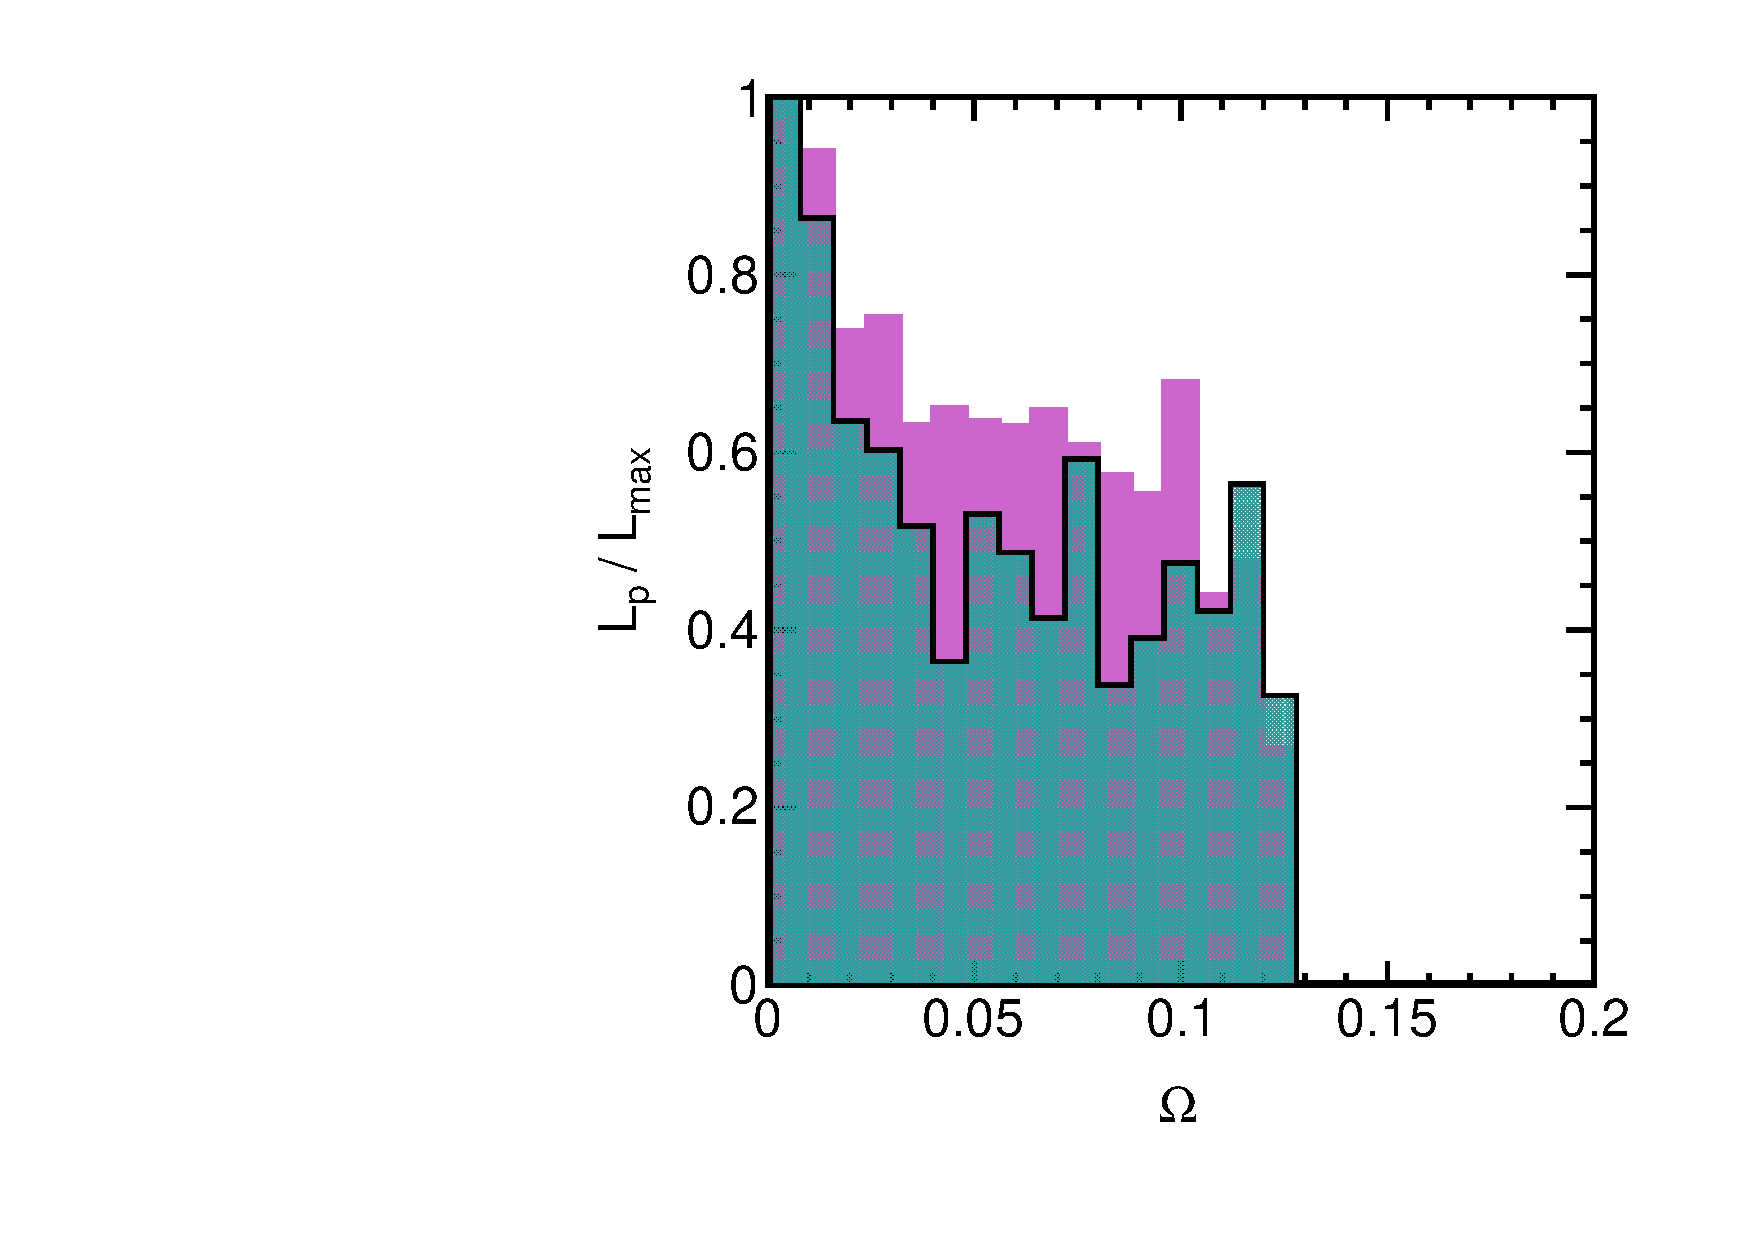
\includegraphics[height=5.5cm]{figs/fig_omega_m.pdf} 
\caption{Ratio of profile likelihood $L_p$ to maximum likelihood $L_{max}$ shown for lightest neutralino dark matter relic density.  The colored and shaded histograms show the distributions before and after the inclusion of the CMS results.}
\label{fig:LRwcms_omg}
\end{center}
\end{figure}


%\begin{figure}[htbp]
%\begin{center}
%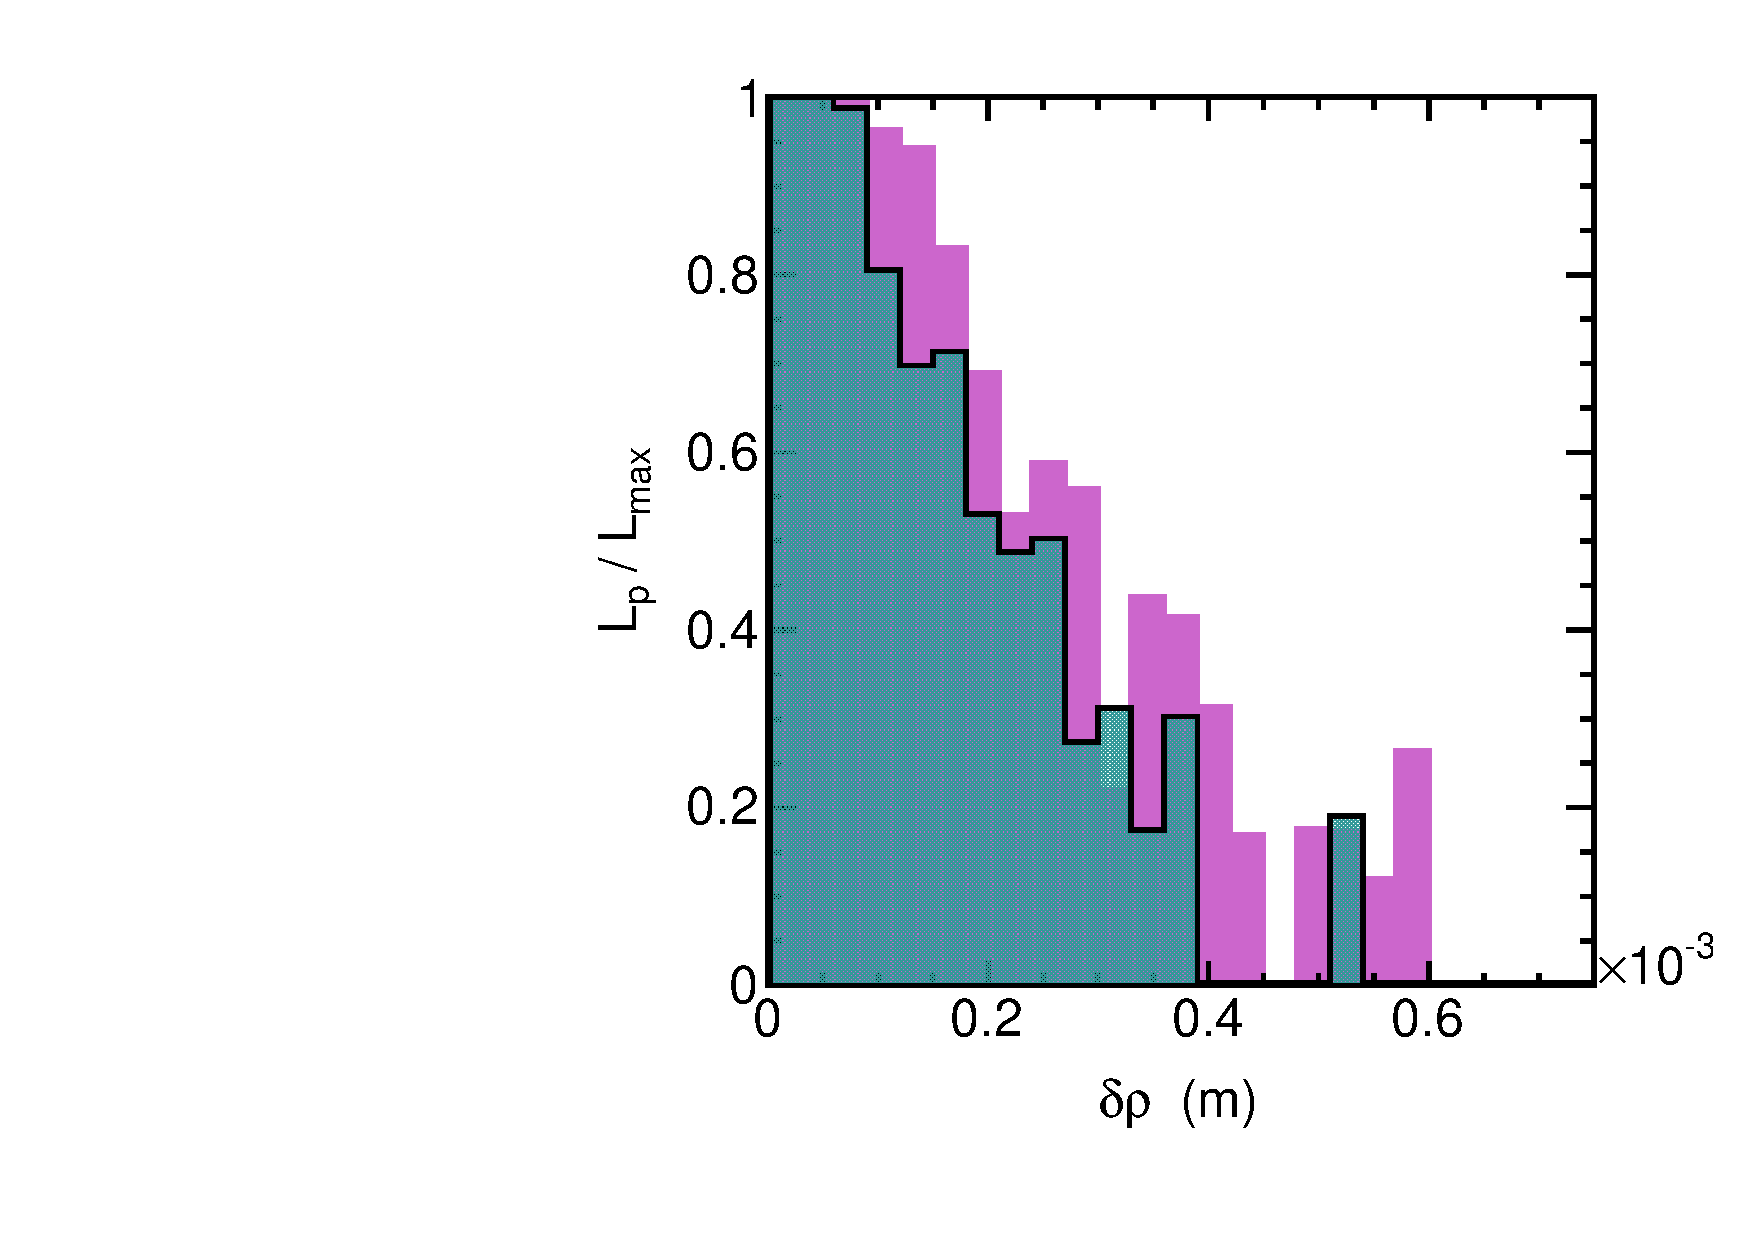
\includegraphics[height=5.5cm]{figs/fig_drho_m.pdf} 
%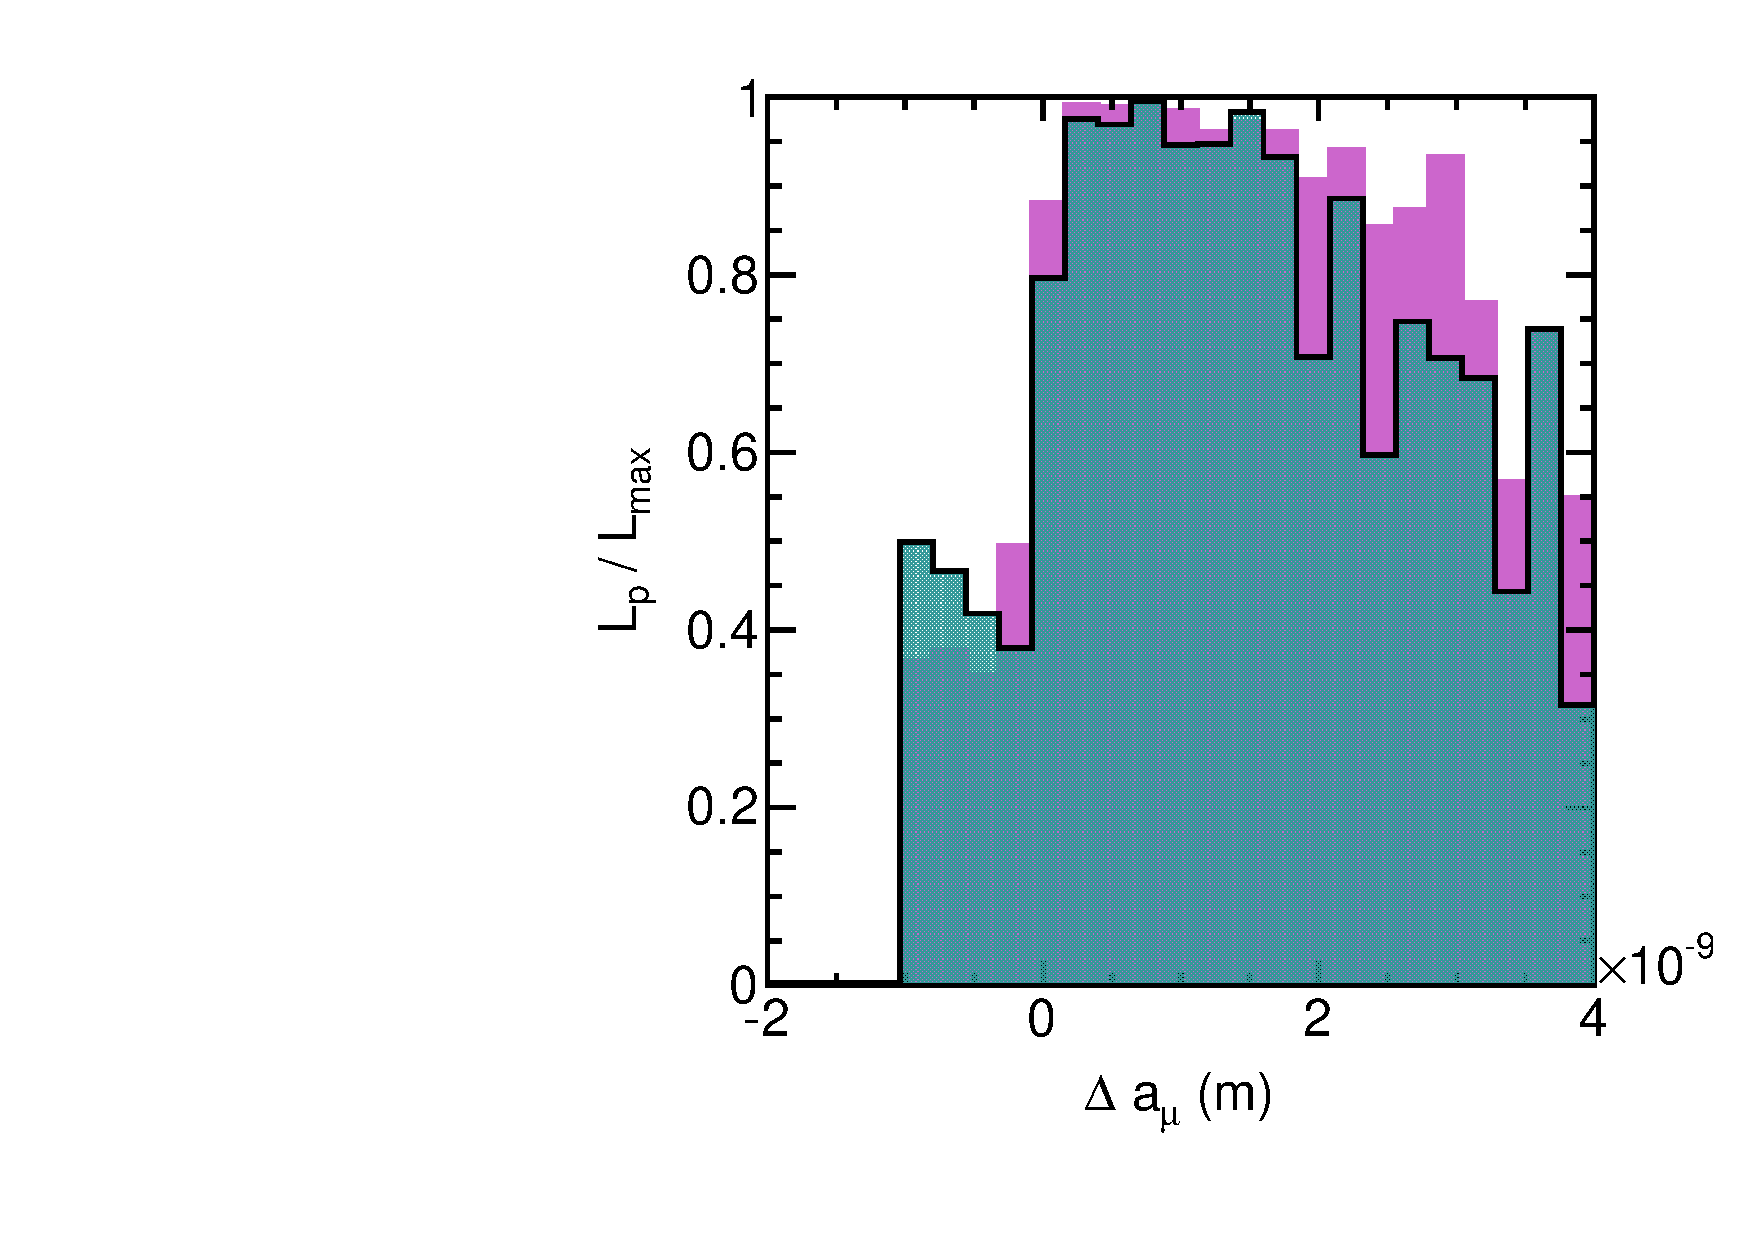
\includegraphics[height=5.5cm]{figs/fig_gmu_m.pdf} \\
%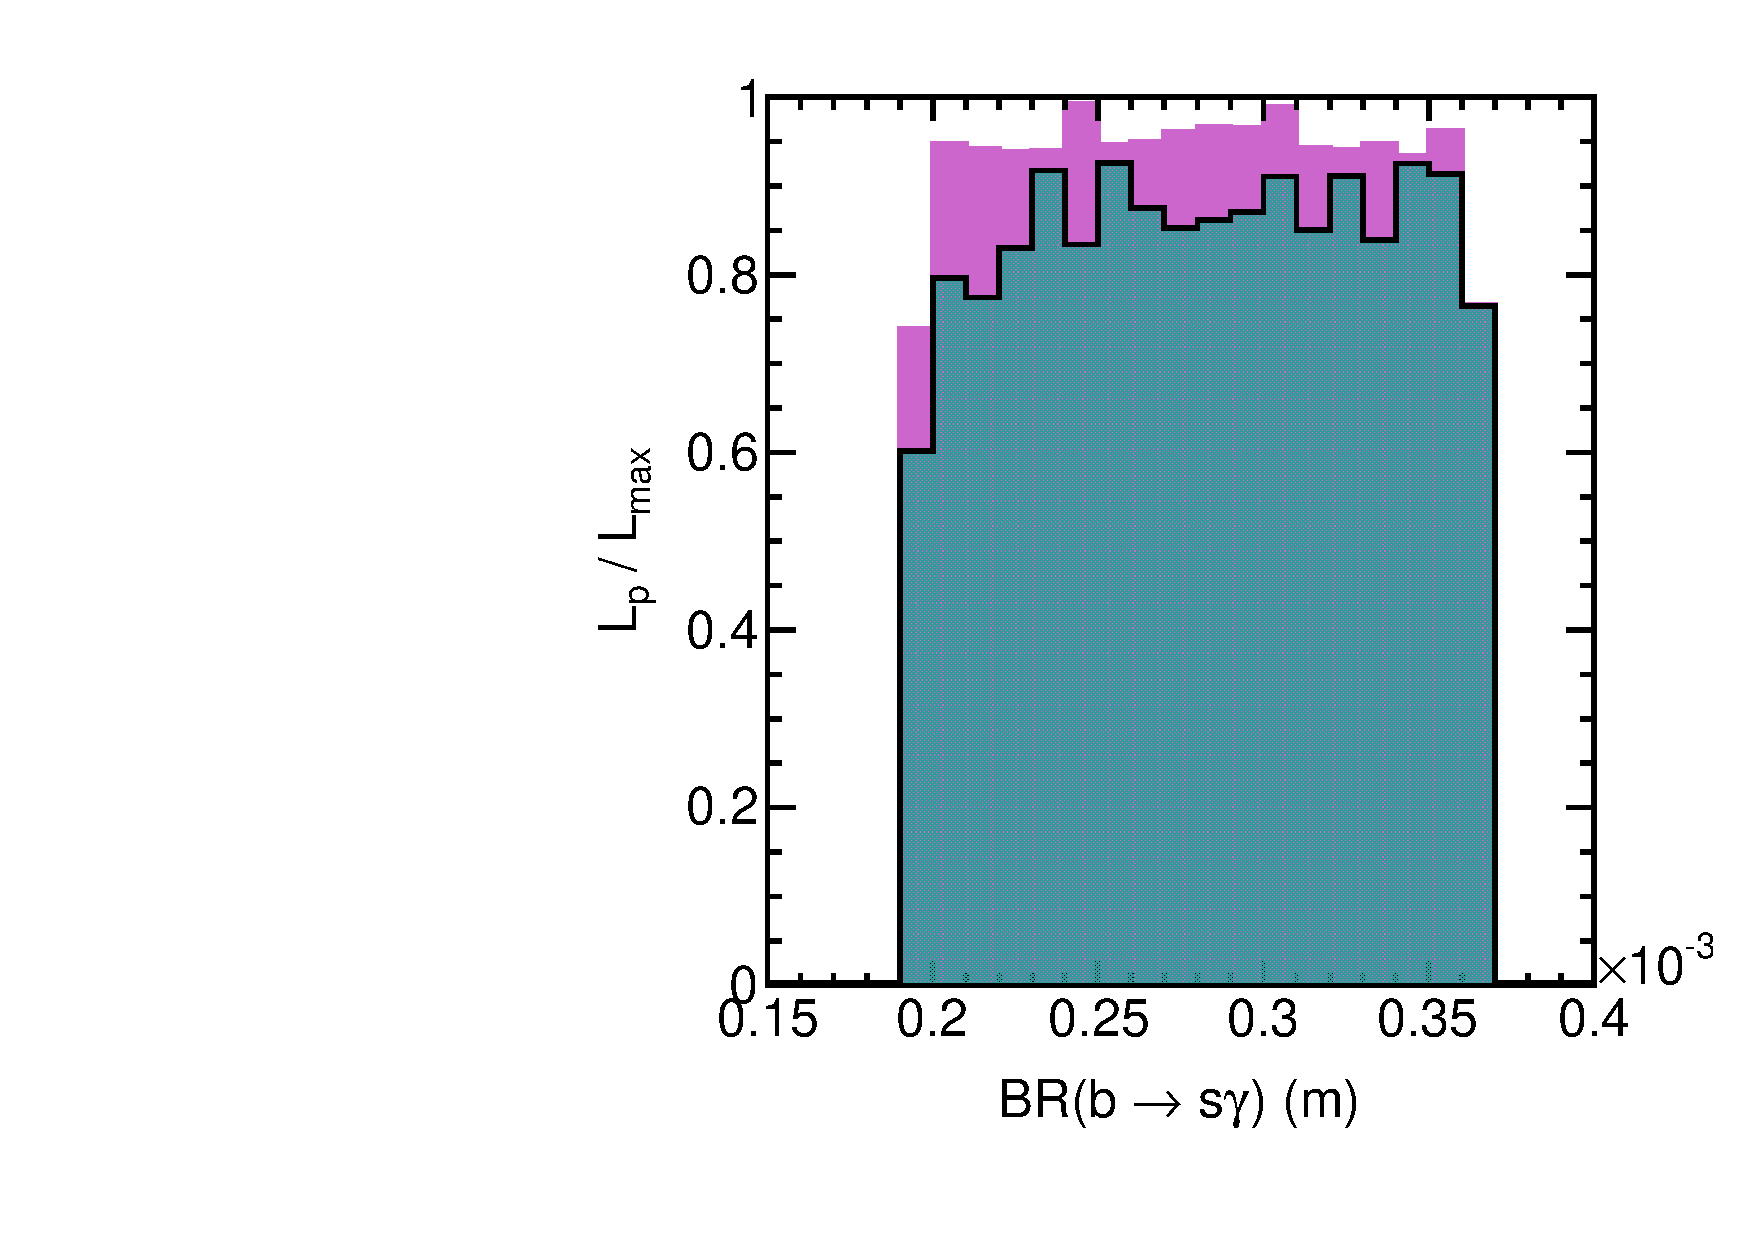
\includegraphics[height=5.5cm]{figs/fig_bsgamma_m.pdf} 
%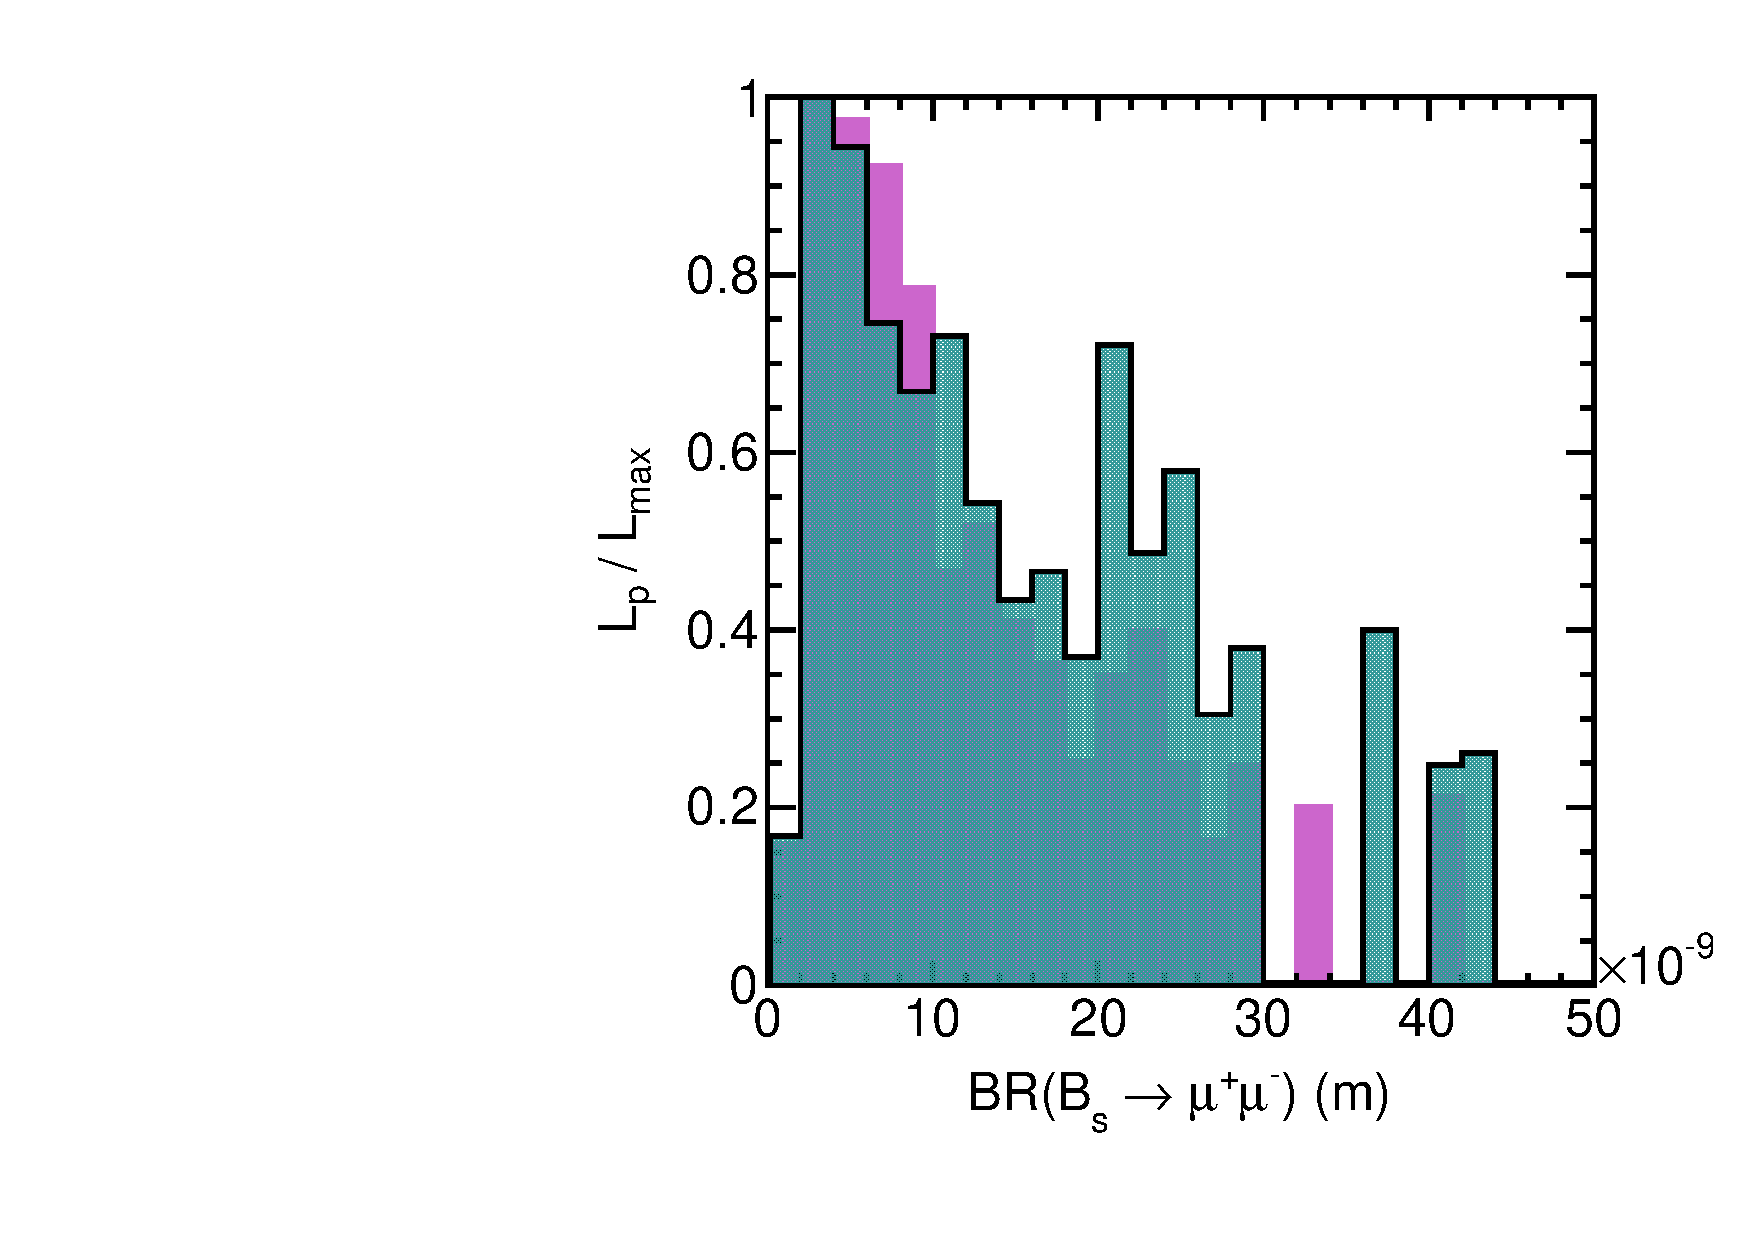
\includegraphics[height=5.5cm]{figs/fig_bsmumu_m.pdf} \\
%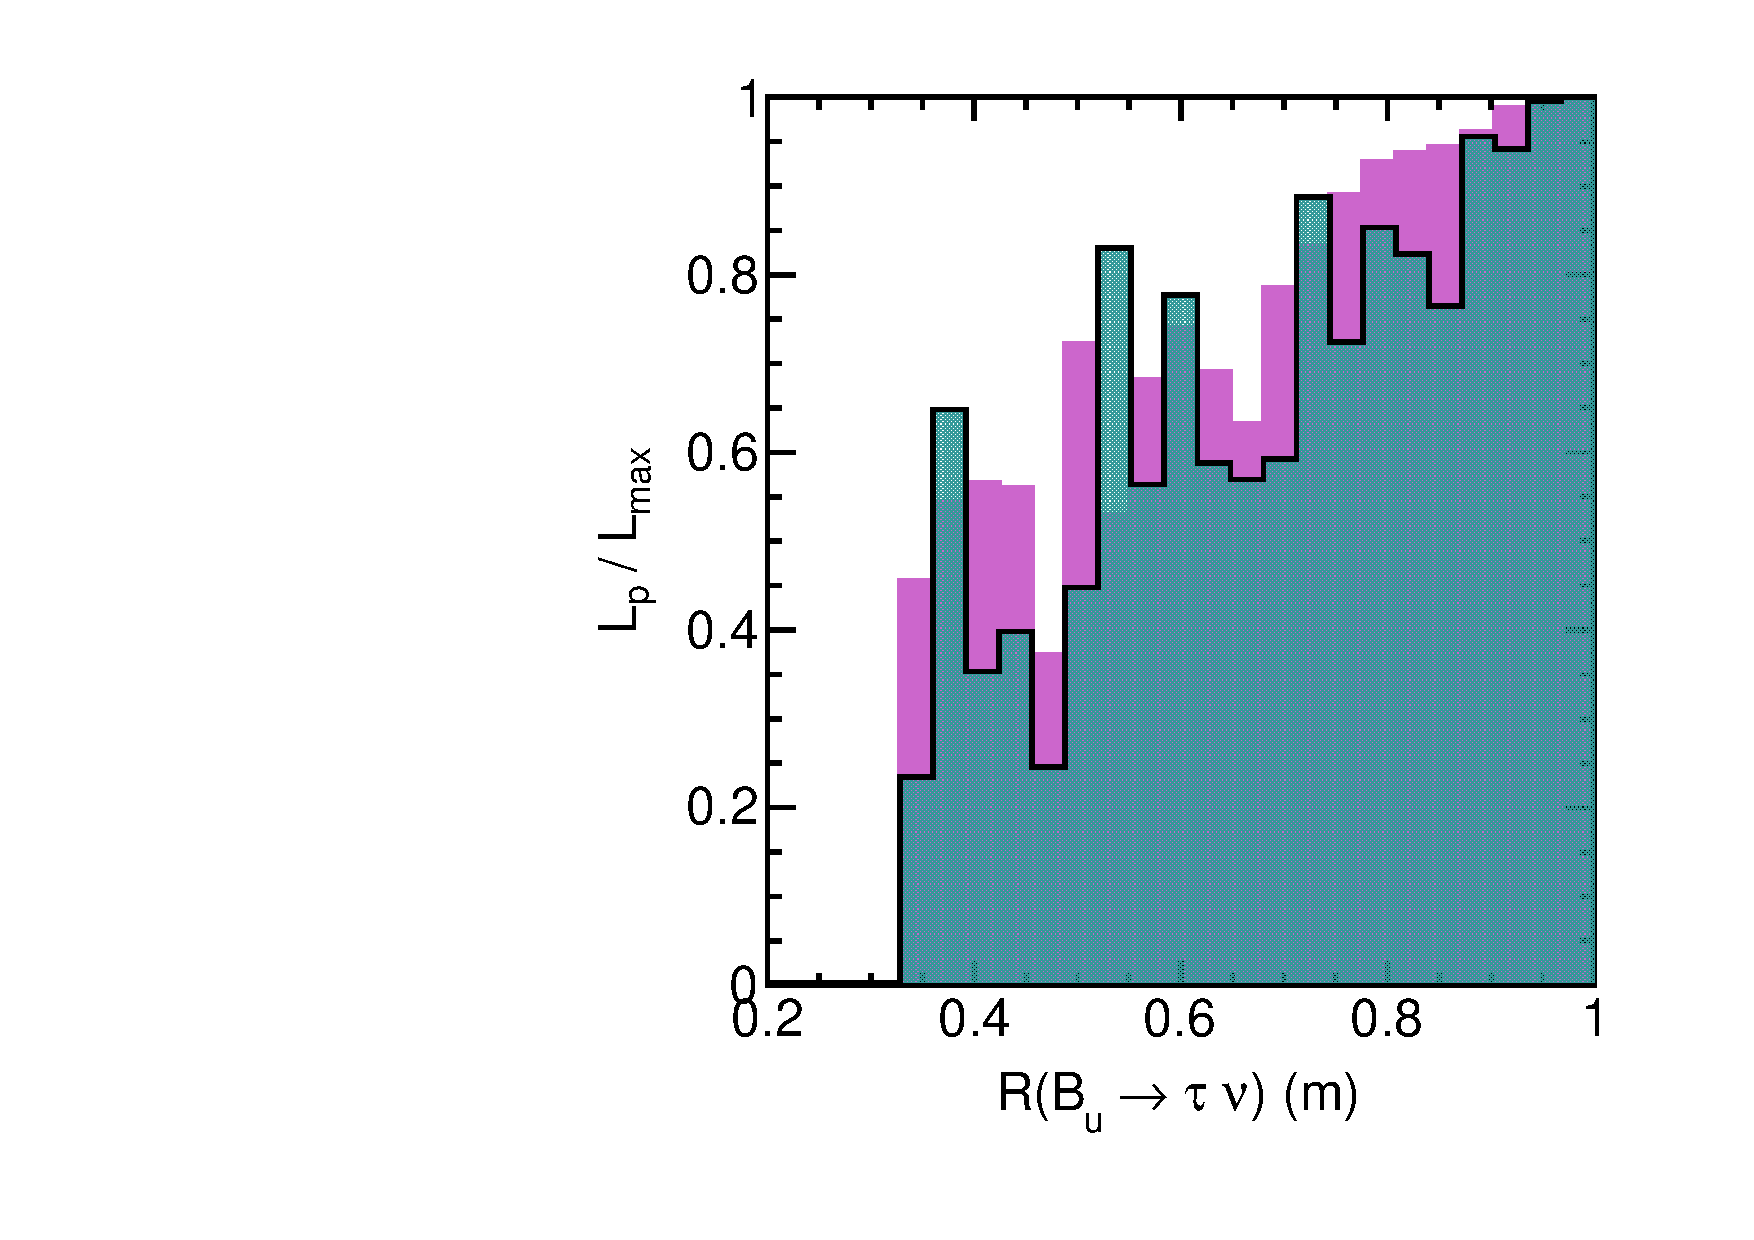
\includegraphics[height=5.5cm]{figs/fig_rbtaunu_m.pdf} 
%\caption{Ratios of profile likelihood $L_p$ to maximum likelihood $L_{max}$ shown for predictions for weak scale observables as calculated by micromegas.  The colored and shaded histograms show the distributions before and after the inclusion of the CMS results.}
%\label{fig:LRwcms_EWobs_m}
%\end{center}
%\end{figure}


\begin{figure}[htbp]
\begin{center}
%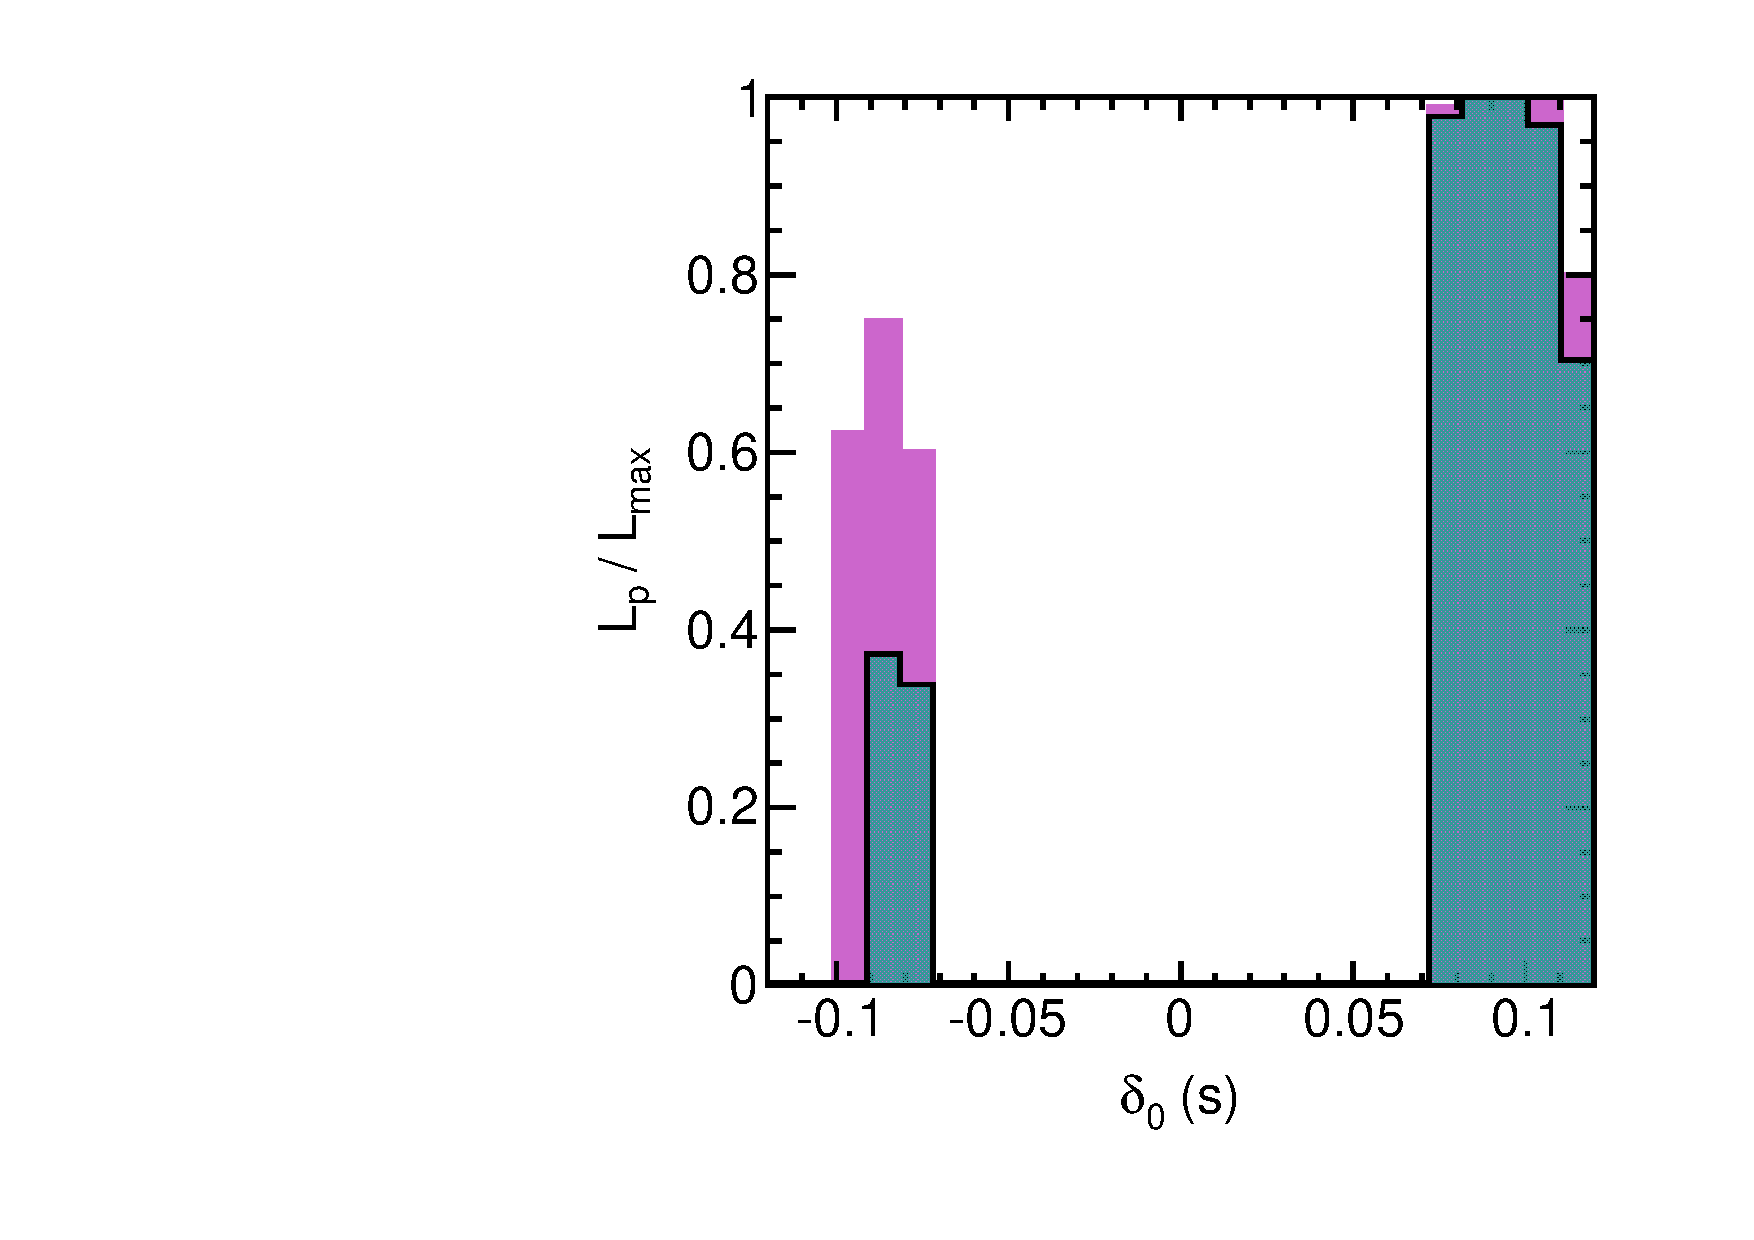
\includegraphics[height=5.5cm]{figs/fig_delta0_s.pdf} 
\includegraphics[height=5.5cm]{figs/fig_drho_m.pdf} 
\includegraphics[height=5.5cm]{figs/fig_muon_gm2_s.pdf} \\
\includegraphics[height=5.5cm]{figs/fig_bsgamma_s.pdf} 
\includegraphics[height=5.5cm]{figs/fig_Bsmumu_s.pdf} \\
\includegraphics[height=5.5cm]{figs/fig_Btaunu_s.pdf} 
\includegraphics[height=5.5cm]{figs/fig_RBtaunu_s.pdf} 
\caption{Ratios of profile likelihood $L_p$ to maximum likelihood $L_{max}$ shown for predictions for weak scale observables.  $\delta\rho$ is calculated using {\tt micrOMEGAs 2.4} and the rest are calculated using {\tt Superiso 2.7}.  The colored and shaded histograms show the distributions before and after the inclusion of the CMS results.}
\label{fig:LRwcms_EWobs_s1}
\end{center}
\end{figure}


\begin{figure}[htbp]
\begin{center}
\includegraphics[height=5.5cm]{figs/fig_BDtaunu_s.pdf} 
\includegraphics[height=5.5cm]{figs/fig_BDtaunu_BDenu_s.pdf} \\
\includegraphics[height=5.5cm]{figs/fig_Dmunu_s.pdf} 
\includegraphics[height=5.5cm]{figs/fig_Dsmunu_s.pdf} \\
\includegraphics[height=5.5cm]{figs/fig_Dstaunu_s.pdf} 
\includegraphics[height=5.5cm]{figs/fig_Kmunu_pimunu_s.pdf} \\
\includegraphics[height=5.5cm]{figs/fig_Rl23_s.pdf} 
\caption{Ratios of profile likelihood $L_p$ to maximum likelihood $L_{max}$ shown for predictions for weak scale observables as calculated by {\tt Superiso 2.7}.  The colored and shaded histograms show the distributions before and after the inclusion of the CMS results.}
\label{fig:LRwcms_EWobs_s2}
\end{center}
\end{figure}






\section{Conclusion}
\label{sec:conclusion}

We have assessed the sensitivity to mSUGRA of a generic signal characterized by two isolated, high $p_T$ leptons,
significant jet activity, and \met. We performed a scan of the mSUGRA $m_{0}-m_{1/2}$ parameter space and determined  
the expected excluded region in the case of no observed signal as well as the $5\sigma$ sensitivity reach for both SS
and OS dileptons, assuming integrated luminosities of 100 pb$^{-1}$ and 1 fb$^{-1}$. Our results indicate that we are sensitive to a
significant region of the mSUGRA parameter space which extends upon previous results from the Tevatron. 




\section*{Acknowledgements}

We thank JoAnne Hewett and Thomas G. Rizzo for providing us the 6K pMSSM points used in this analysis.



% ---- references ----
%\bibliographystyle{h-physrev}
%\bibliography{pmssm}
\clearpage
\begin{thebibliography}{10}

\bibitem{Choi:2007ka}
K.~Choi and H.~P. Nilles,
\newblock JHEP {\bf 04}, 006 (2007), hep-ph/0702146.

\bibitem{Martin:2009ad}
S.~P. Martin,
\newblock Phys. Rev. {\bf D79}, 095019 (2009), 0903.3568.

\bibitem{Horton:2009ed}
D.~Horton and G.~G. Ross,
\newblock Nucl. Phys. {\bf B830}, 221 (2010), 0908.0857.

\bibitem{Allanach:2006fy}
B.~C. Allanach {\em et~al.},
\newblock (2006), hep-ph/0602198.

\bibitem{Kolda:1995iw}
C.~F. Kolda and S.~P. Martin,
\newblock Phys. Rev. {\bf D53}, 3871 (1996), hep-ph/9503445.

\bibitem{Polonsky:1994sr}
N.~Polonsky and A.~Pomarol,
\newblock Phys. Rev. Lett. {\bf 73}, 2292 (1994), hep-ph/9406224.

\bibitem{Polonsky:1994rz}
N.~Polonsky and A.~Pomarol,
\newblock Phys. Rev. {\bf D51}, 6532 (1995), hep-ph/9410231.

\bibitem{Ellis:2002wv}
J.~R. Ellis, K.~A. Olive, and Y.~Santoso,
\newblock Phys. Lett. {\bf B539}, 107 (2002), hep-ph/0204192.

\bibitem{Berger:2008cq}
C.~F. Berger, J.~S. Gainer, J.~L. Hewett, and T.~G. Rizzo,
\newblock JHEP {\bf 02}, 023 (2009), 0812.0980.

\bibitem{Conley:2010du}
J.~A. Conley, J.~S. Gainer, J.~L. Hewett, M.~P. Le, and T.~G. Rizzo,
\newblock (2010), 1009.2539.

\bibitem{Lyons:2003bw}
L.~Lyons, (ed.~), R.~P. Mount, (ed.~), and R.~Reitmeyer, (ed.~),
\newblock Prepared for PHYSTAT2003: Statistical Problems in Particle Physics,
  Astrophysics, and Cosmology, Menlo Park, California, 8-11 Sep 2003.

\bibitem{Nakamura:2010zzi}
Particle Data Group, K.~Nakamura,
\newblock J. Phys. {\bf G37}, 075021 (2010).

\bibitem{top:1900yx}
CDF and D0, and others,
\newblock (2010), 1007.3178.

\bibitem{Schael:2006cr}
{ALEPH, DELPHI, L3 and OPAL collaborations and the LEP Working Group for Higgs
  Boson Searches}, S.~Schael {\em et~al.},
\newblock Eur. Phys. J. {\bf C47}, 547 (2006), hep-ex/0602042.

\bibitem{Degrassi:2002fi}
G.~Degrassi, S.~Heinemeyer, W.~Hollik, P.~Slavich, and G.~Weiglein,
\newblock Eur. Phys. J. {\bf C28}, 133 (2003), hep-ph/0212020.

\bibitem{Davier:2010nc}
M.~Davier, A.~Hoecker, B.~Malaescu, and Z.~Zhang,
\newblock (2010), 1010.4180.

\bibitem{HFAG:2010qj}
The Heavy Flavor Averaging Group, D.~Asner {\em et~al.},
\newblock (2010), 1010.1589.

\bibitem{Jarosik:2010iu}
N.~Jarosik {\em et~al.},
\newblock (2010), 1001.4744.

\bibitem{lepsusy}
ALEPH, DELPHI, L3 and OPAL, {LEP2 SUSY Working Group,},
\newblock {\tt http://lepsusy.web.cern.ch/lepsusy/}.

%\cite{Skands:2003cj}
\bibitem{Skands:2003cj}
  P.~Z.~Skands {\it et al.},
  %``SUSY Les Houches Accord: Interfacing SUSY Spectrum Calculators, Decay
  %Packages, and Event Generators,''
  JHEP {\bf 0407} (2004) 036
  [arXiv:hep-ph/0311123].
  %%CITATION = JHEPA,0407,036;%%

%\cite{Sjostrand:2006za}
\bibitem{Sjostrand:2006za}
  T.~Sjostrand, S.~Mrenna and P.~Z.~Skands,
  %``PYTHIA 6.4 Physics and Manual,''
  JHEP {\bf 0605} (2006) 026
  [arXiv:hep-ph/0603175].
  %%CITATION = JHEPA,0605,026;%%

%\cite{Ovyn:2009tx}
\bibitem{Ovyn:2009tx}
  S.~Ovyn, X.~Rouby and V.~Lemaitre,
  %``Delphes, a framework for fast simulation of a generic collider
  %experiment,''
  arXiv:0903.2225 [hep-ph].
  %%CITATION = ARXIV:0903.2225;%%
%
\bibitem{Belanger:2006is}
  G.~Belanger, F.~Boudjema, A.~Pukhov and A.~Semenov,
  %``micrOMEGAs2.0: A program to calculate the relic density of dark matter  in
  %a generic model,''
  Comput.\ Phys.\ Commun.\  {\bf 176}, 367 (2007)
  [arXiv:hep-ph/0607059].
  %%CITATION = CPHCB,176,367;%%
%
\bibitem{Mahmoudi:2008tp}
  F.~Mahmoudi,
  %``SuperIso v2.3: A Program for calculating flavor physics observables in
  %Supersymmetry,''
  Comput.\ Phys.\ Commun.\  {\bf 180}, 1579 (2009)
  [arXiv:0808.3144 [hep-ph]].
  %%CITATION = CPHCB,180,1579;%%
%


\end{thebibliography}


% ---- appendix ----
\clearpage
\appendices
\section*{Appendices}
\section{Comparison of kinematic quantities with full simulation}
\label{sec:cmsdelphescomp}
We compare the important kinematic variables used for the study with the CMSSW full
simulation using the LM1 benchmark point. Figures~\ref{fig:njetht},~\ref{fig:jetpteta},~\ref{fig:alphat}
show that the simulation using our {\tt Delphes}-based infrastructure agree well with the full simulation.

\begin{figure}[htbp]
\begin{center}
\includegraphics[height=5.5cm]{figs/njetht.pdf} 
\caption{Distributions using the CMSSW full simulation and {\tt Delphes} for the LM1 benchmark point as a function of jet multiplicity (left) and $H_T$ (right)}.
\label{fig:njetht}
\end{center}
\end{figure}


\begin{figure}[htbp]
\begin{center}
\includegraphics[height=5.5cm]{figs/jet1pteta.pdf} 
\caption{Distributions using the CMSSW full simulation and {\tt Delphes} for the LM1 benchmark point 
as a function of jet pseudorapidity (left) and $p_T$ (right)}.
\label{fig:jetpteta}
\end{center}
\end{figure}

\begin{figure}[htbp]
\begin{center}
\includegraphics[height=9.cm]{figs/alphat.pdf} 
\caption{Distributions using the CMSSW full simulation and {\tt Delphes} for the LM1 benchmark point
as a function of $\alpha_{T}$ (top left), $\Delta \phi^{*}$ (top right) and MHT/MET (bottom)}.
\label{fig:alphat}
\end{center}
\end{figure}


\clearpage
\section*{Appendix}
\label{sec:stat}
We describe the (frequentist) 
statistical procedures we have used in this study.  Suppose 
that our goal is to make a statement about the parameter $\theta_1$,
say the gluino mass
parameter $M_3$, independently of the remaining 18 pMSSM parameters. Since the 
expected signal $s$ is a function of  $d = 19$ parameters (see Sect.~(\ref{sec:pmssm}),
which we denote by $\theta = \theta_1,\cdots,\theta_{19}$,  we need to eliminate $d - 1$ of them from the likelihood function so that the latter becomes a function of $\theta_1$ only. In general, it is extremely difficult to do this in 
a frequentist calculation in a way that preserves \emph{exact} coverage over the entire parameter
space. However, let $L_p(\theta_1) \equiv L(\theta_1, \hat{\theta}_2(\theta_1), \cdots)$ be the 
1-dimensional \emph{profile likelihood}, that is, the function obtained by maximizing the likelihood function $L(\theta_1, \theta_2, \cdots, \theta_{19})$ with respect to $\theta_2,\cdots,\theta_{19}$ for \emph{fixed} $\theta_1$ and replacing the exact, but unknown, values of $\theta_2,\cdots,\theta_{19}$
by their maximum likelihood estimates (MLE),  $\hat{\theta}_2(\theta_1),\cdots,\hat{\theta}_{19}(\theta_1)$. 

Replacing exact values by estimates is clearly an approximation. We should therefore not
expect any procedure that uses this approximation to yield confidence limits and intervals
with exact coverage. However, in practice, 1-dimensional profile likelihoods created from
multi-parameter likelihood functions often perform
surprisingly well~\cite{James}.
Let $L_{max}$ be the maximum of the likelihood function $L(\theta)$ and let 
$\Lambda = L_p /  L_{max}$ be the likelihood ratio. 
If the partial derivatives with respect to $\theta_i$ of the likelihood function, $L(\theta)$, exist up to second order and they form a $d \times d$ non-singular matrix (the Hessian), 
the following result holds,
\begin{equation}
    W = -2\log\Lambda \rightarrow \chi^2,
\end{equation}
as the amount of data grows without limit. This is  Wilks theorem~\cite{Wilks, James}. For an 
approximate 95\% C.L. lower limit on $\theta_1$, we set $W = 1.64$, that is, $\Lambda = 0.44$,
and solve for the lower limit.

\subsection*{Non-parametric profiling algorithm}
The problem we need to solve is the following: for a fixed value of a parameter, say $Q$, we want to find 
the maximum value of the likelihood function when the latter is available only as a weighted swarm of points. The quantity $Q$ could be a pMSSM parameter, a predicted observable of a 
sparticle mass. Here, written as pseudo-code, is our algorithm for finding the profile likelihood:
\begin{verbatim}
1	pMSSMPOINTS, QBIN, Q = inputs()
2	NBOOTSTRAP = 100
3	profile = 0

4	repeat NBOOTSTRAP times:
	      
5	      POINTS = generateBootstrapSample(pMSSMPOINTS)
6	      histogram = histogramPoints(POINTS)
	
7	      DMAX = -1
8	      for point in POINTS:
	      
9	           if Q not in QBIN: continue
	      
10	           d = histogram.density(point)	      
11	           if d > DMAX: DMAX = d
	 
12	      profile = profile + DMAX
	        
13	 profile = profile / NBOOTSTRAP	 
14	 return profile	      
\end{verbatim}
\begin{itemize}
	\item[1] Get the pMSSM points, the bin $QBIN$ for which the profile likelihood
	is to be computed, and the value of $Q$.
	
	\item[6] Generate a $d$-dimensional histogram from current bootstrap sample.
	
	\item[9] Make sure $Q$ lies in desired bin $QBIN$.
	
	\item[10,11] Find largest density $DMAX$ so far.
	
	\item[12--14] Return average of estimates of profile likelihood.
\end{itemize}
The above algorithm is implemented in a class we developed called {\tt KDTProfileLikelihood}, which
makes use of the multi-dimensional histogrammer {\tt TKDTreeBinning} in Root.
The $d$-dimensional histogram is created through recursive binary partitioning of the parameter
space in such a way that bins have equal counts. The underlying data structure is 
a kd-tree~\cite{TKDTreeBinning}.

\subsection*{Comparison of kinematic quantities with Full Simulation}
\label{sec:compare}
We compare the important kinematic variables used for the study with the CMSSW 
Full simulation using LM1 benchmark point. Figures~\ref{fig:njetht},~\ref{fig:jetpteta},~\ref{fig:alphat}
shows that the simulation/reconstruction infrastructure used agree well with the full simulation.

\begin{figure}[htbp]
\begin{center}
\includegraphics[height=5.5cm]{figs/njetht.pdf} 
\caption{Event distribution using CMSSW Full simulation along with Delphes for LM1 benchmark points, 
as a function of jet multiplicity (left) and $H_T$ (right)}
\label{fig:njetht}
\end{center}
\end{figure}


\begin{figure}[htbp]
\begin{center}
\includegraphics[height=5.5cm]{figs/jet1pteta.pdf} 
\caption{Event distribution using CMSSW Full simulation along with Delphes for LM1 benchmark points, 
as a function of pseudorapidity (left) and $p_T$ of the jets (right)}
\label{fig:jetpteta}
\end{center}
\end{figure}

\begin{figure}[htbp]
\begin{center}
\includegraphics[height=9.cm]{figs/alphat.pdf} 
\caption{Event distribution using CMSSW Full simulation along with Delphes for LM1 benchmark points, 
as a function of $\alpha_{T}$ (top left), $\Delta \phi^{*}$ (top right) and MHT/MET (bottom)}
\label{fig:alphat}
\end{center}
\end{figure}


%\begin{thebibliography}
%	\bibitem{Wilks}
%	S.S~Wilks, ``The large-sample distribution of the likelihood ratio for testing composite hypotheses,'' Ann. Math. Statist. {\bf 9}, 60-62 (1938).
%	
%	\bibitem{James}
%	F.~James, ``Statistical Methods in Experimental Physics,''  2nd Edition, (World Scientific, Singapore, 2008).
%	
%\end{thebibliography}


\end{document}
